\documentclass[12pt,a4paper]{article}

\usepackage[a4paper,margin=2.54cm,top=2.8cm,bottom=2.8cm]{geometry}
\usepackage[T1]{fontenc}
\usepackage[utf8]{inputenc}
\usepackage{newtxtext}
\usepackage{newtxmath}
\usepackage{microtype}
\usepackage{setspace}
\usepackage{booktabs}
\usepackage{longtable}
\usepackage{needspace}
\usepackage{array}
\usepackage{tabularx}
\usepackage{multirow}
\usepackage{graphicx}
\usepackage{caption}
\usepackage{subcaption}
\usepackage{float}
\usepackage[section]{placeins}
\usepackage{amsmath}
\usepackage{enumitem}
\usepackage{fancyhdr}
\usepackage{lastpage}
\usepackage{pdflscape}
\usepackage[round,authoryear]{natbib}
\usepackage[colorlinks=true,linkcolor=blue,citecolor=blue,urlcolor=blue]{hyperref}
\usepackage{nameref}

\setstretch{1.15}
\setlength{\parindent}{0.5in}
\setlength{\parskip}{0pt}
\setlength{\headheight}{14.5pt}
\setlength{\textfloatsep}{10pt plus 2pt minus 2pt}
\setlength{\intextsep}{8pt plus 2pt minus 2pt}
\setlist[itemize]{leftmargin=1.6em, itemsep=2pt, topsep=4pt}
\setlist[enumerate]{leftmargin=1.8em, itemsep=2pt, topsep=4pt}

\pagestyle{fancy}
\fancyhf{}
\fancyhead[L]{\small\textit{Cognitive Bias Vulnerability in Cyber Context}}
\fancyhead[R]{\small\thepage}
\renewcommand{\headrulewidth}{0.4pt}
\renewcommand{\footrulewidth}{0pt}

\DeclareCaptionLabelSeparator{apasep}{\\}
\captionsetup{
  font=small,
  labelfont=bf,
  textfont=it,
  labelsep=apasep,
  justification=raggedright,
  singlelinecheck=false,
  skip=6pt
}
\captionsetup[table]{position=above}
\captionsetup[figure]{position=above}
\captionsetup[longtable]{
  font=small,
  labelfont=bf,
  textfont=it,
  labelsep=apasep,
  justification=raggedright,
  singlelinecheck=false,
  width=\textwidth
}
\setlength{\LTcapwidth}{\textwidth}
\setlength{\LTleft}{0pt}
\setlength{\LTright}{0pt}

\newcommand{\ecbss}{\textsc{ECBSS}}
\newcommand{\vacus}{V-A-C-U-S}
\newcommand{\fignote}[1]{%
  \par\vspace{3pt}\noindent%
  \begin{minipage}{0.96\linewidth}\footnotesize\raggedright\textit{Note.}~#1\end{minipage}%
}
\newcommand{\tabnote}[1]{%
  \par\vspace{3pt}\noindent%
  \begin{minipage}{0.96\linewidth}\footnotesize\raggedright\textit{Note.}~#1\end{minipage}%
}

\begin{document}
\emergencystretch=2em

\begin{titlepage}
\thispagestyle{empty}
\vspace*{1.4cm}
\begin{center}
{\fontsize{18}{22}\selectfont\bfseries Cognitive Bias Vulnerability Across Emotional States\\[2pt] in Cyber-Relevant Decision Contexts\par}
\vspace{1.8cm}
{\large Stijn Van Severen\textsuperscript{1,*}\par}
\vspace{0.30cm}
{\normalsize \textsuperscript{1} Ghent University, Ghent, Belgium\par}
\vspace{0.15cm}
{\normalsize \textsuperscript{*}Corresponding author: \href{mailto:stijn.vanseveren@ugent.be}{stijn.vanseveren@ugent.be}\par}
\end{center}
\vspace{1.0cm}
\begin{center}
\textbf{Abstract}
\end{center}
\begin{center}
\begin{minipage}{0.92\textwidth}
Human-centered cybersecurity failures are increasingly traced to transient emotional states that modulate cognitive-bias vulnerability, yet no unified framework maps this interaction across the full space of documented cyber-relevant biases and emotional states. This study introduces a multi-layer taxonomy of 200 cognitive biases for cyber-relevant environments nested in 40 clusters and 11 families, then estimates how 239 emotion states shift family-level vulnerability across all 2,629 pairings. Each emotion was scored on five affective components (i.e., valence, arousal, control/coping, uncertainty, and social orientation; \vacus{}) using structured zero-temperature large-language-model judging, and family-level Emotion-Conditioned Bias Shift Scores (\ecbss{}, $-1000$ to $+1000$) were derived from the same pipeline. Most emotion-family pairs amplified cognitive-bias susceptibility (77.6\%; grand mean $= 368.8$, $SD = 472.8$). Mixed-effects modeling identified arousal as the strongest amplifier ($\beta = 504.1$, $SE = 20.8$, $p < .001$) and perceived control as the strongest attenuator ($\beta = -542.3$, $SE = 32.0$, $p < .001$); uncertainty also attenuated scores counterintuitively ($\beta = -357.1$, $p < .001$), whereas social orientation was negligible ($p = .925$). Six emotion clusters showed distinct vulnerability profiles: high-arousal positive states produced the highest mean \ecbss{} (581.8) and withdrawn low-arousal states the lowest (111.5). Variance decomposition assigned similar shares to emotion cluster ($\eta^2 = .093$) and bias family ($\eta^2 = .097$), with 81.0\% of variance residing in pair-specific residuals. Altogether, these findings support the need for component-sensitive models of affective risk and point toward affect-informed cybersecurity training and interface design.
\end{minipage}
\end{center}
\end{titlepage}

\clearpage
\setcounter{page}{1}

%% ============================================================
\section{Introduction}
%% ============================================================

\subsection{The Human Element in Cybersecurity}

Cybersecurity capabilities have improved rapidly across governance, architecture, and detection engineering \citep{verizon2025dbir, nistcsf2024}. Yet this progress does not eliminate the human-decision layer as a persistent attack surface: unlike software vulnerabilities, moment-to-moment judgment under pressure cannot be patched or updated in a single deployment cycle. Adversaries exploit predictable cognitive shortcuts in authority evaluation, urgency response, and social-cue processing under conditions that are rarely emotionally neutral \citep{workman2008wisecrackers, heartfield2016semantic, stajano2011scam, pfleeger2012leveraging}. The cybersecurity-behavior literature confirms that phishing susceptibility, risk-perception calibration, and compliance behavior vary with psychological and contextual factors \citep{alsharida2023human, althobaiti2024phishing, hadlington2017human}, but there is still no comprehensive map linking the full emotional-state space to the full taxonomy of cyber-relevant cognitive biases.

\subsection{Emotional Differentiation in Cyber Environments}

Dual-process accounts of judgment and decision-making distinguish fast, associative, heuristic processing (System~1) from slower, deliberative, rule-governed reasoning (System~2) \citep{kahneman2011thinking, evans2008dual, stanovich2000individual}. Cognitive biases represent predictable misfirings of System~1 heuristics when those heuristics are applied to contexts for which they are poorly calibrated \citep{tversky1974judgment}. The balance between processing modes is not fixed: it shifts with time pressure, cognitive load, and activation states---exactly the conditions adversaries manufacture in cyber interactions \citep{buckley2023employee, frank2022contextual, hadlington2017human}.

Component-theoretic and cyberpsychology evidence indicates that outcomes depend on differentiated emotional profiles rather than valence alone \citep{lazarus1984stress, smith1985patterns, lerner2000beyond, renaud2021emotions}. Fear and anger are both negatively valenced but produce different risk signatures: fear trends toward risk aversion, whereas anger trends toward certainty-based risk taking \citep{lerner2000beyond, lerner2015emotion}. The affect-infusion model \citep{forgas1995mood}, risk-as-feelings \citep{loewenstein2001risk}, and affect-heuristic framework \citep{slovic2007affect} converge on a common implication for cybersecurity: manipulations that increase activation and reduce perceived coping capacity can shift decision mode toward heuristic shortcuts that social-engineering tactics are designed to exploit.

\subsection{Cybersecurity Emotion Research: State and Gaps}

Empirical cyber-behavior research has begun to engage with emotion \citep{renaud2021emotions, vanSchaik2020risk}, and multiple studies show that phishing susceptibility varies with impulsivity, attention control, and emotional processing differences \citep{vishwanath2011people, buckley2023employee, frank2022contextual, beltz2025gambit}. Risk perception in security contexts is affect-laden, consistent with emotion-informed judgment models \citep{vanSchaik2020risk}. However, current evidence remains fragmented: constructs are operationalized inconsistently, induction paradigms vary across labs, and no prior study maps emotional modulation across a full cyber-relevant bias taxonomy \citep{alsharida2023human, althobaiti2024phishing, renaud2021emotions}. The key unresolved gap is structural: the field lacks a shared, theory-grounded representation that connects the complete emotion lexicon to the complete cognitive-bias taxonomy in one coherent analytical framework.

\subsection{The Present Study and Research Questions}

This study addresses that gap through an end-to-end structured knowledge-elicitation pipeline combining taxonomy construction, affective-dimension emotion modeling, structured large-language-model (\textsc{LLM}) scoring, and robustness analyses. Large-language models are increasingly used as population-level simulators for psychologically structured inference tasks \citep{argyle2023out, grossmann2023ai}. Four research questions (RQs) guided the confirmatory analyses:

\begin{enumerate}[label=RQ\arabic*.,leftmargin=2.8em]
  \item Do emotional states systematically shift cognitive bias vulnerability in cyber-relevant decision contexts?
  \item Which affective dimensions (valence, arousal, control/coping, uncertainty, social orientation) are the primary predictors of vulnerability amplification or attenuation?
  \item Do distinct emotion clusters produce qualitatively different vulnerability profiles across the bias taxonomy?
  \item Does the dimension-based account outperform a simple valence-based model in explaining vulnerability variance?
\end{enumerate}

%% ============================================================
\section{Methods}
%% ============================================================

\subsection{Taxonomy Construction}

A three-level, mechanism-first cognitive-bias taxonomy was constructed through a two-phase iterative process. In the first phase, a recursive scaffold of families, clusters, and leaf biases was generated using the generative scaffolding capabilities of GPT-5.4 \citep{openai2025gpt54}, with mechanism-based grouping as the organizing principle to prevent the taxonomy from collapsing into an alphabetic catalog or duplicate-label list. Eleven bias families were defined at the highest level---each anchored to a distinct cognitive processing domain---with intermediate clusters capturing mechanism-coherent groupings within families and individual leaf biases at the terminal nodes.

In the second phase, this scaffold was manually curated through a PRISMA-informed rapid review \citep{page2021prisma}. Records were identified through broad concept-sensitive searches spanning cognitive psychology, behavioral economics, social psychology, and cybersecurity literatures; screened at title/abstract and full-text stages; and adjudicated through explicit inclusion/exclusion rules documented in the preregistration workflow (Supplementary Figure~\ref{fig:s1}). Inclusion required either (a) direct empirical documentation in cyber or security-adjacent literature, or (b) a theoretically defensible structural mapping to a cyber-relevant decision function---specifically: trust and source-credibility assessment, urgency and temporal-pressure responses, information-search and evidence evaluation, privacy-disclosure and self-presentation decisions, compliance and exception-management, or authority and social-influence processing. Umbrella constructs, disputed synonyms, and ambiguous subtype distinctions were resolved by explicit definitional review; only after consolidation were concepts placed into the taxonomy. The frozen taxonomy contained 200 cognitive biases organized into 40 clusters and 11 families (Figure~\ref{fig:taxonomy}; Supplementary Tables~\ref{tab:s1-taxonomy} and~\ref{tab:s6-taxonomy}).

\subsection{Emotion Lexicon and Affective Component Scoring}

A lexicon of 239 discrete emotion labels was assembled to span the full five-component affective space. Labels were drawn from established taxonomies and lexical resources, including the Differential Emotions framework \citep{izard2007basic}, the Geneva Emotion Wheel \citep{scherer2005emotions}, Plutchik's wheel \citep{plutchik1980emotion}, and the NRC Emotion Lexicon \citep{mohammad2013crowdsourcing}. The lexicon was supplemented to ensure representation across the full range of each component: high-arousal threat states (e.g., \textit{terrified}, \textit{panicked}), affiliative and socially positive states (e.g., \textit{adoring}, \textit{trusting}), low-arousal withdrawal states (e.g., \textit{numb}, \textit{detached}), antagonistic high-control states (e.g., \textit{contemptuous}, \textit{defiant}), and mixed socially evaluative states (e.g., \textit{envious}, \textit{guilty}). Near-synonyms were retained only when their expected profiles differed on at least one key component. Full label-level values are listed in Supplementary Table~\ref{tab:s8-emotions}.

Each emotion was scored on the \vacus{} component framework: Valence (positive vs.\ negative hedonic tone), Arousal (physiological and attentional activation), Control/coping (perceived ability to manage the situation), Uncertainty (subjective ambiguity about the situation and its outcome), and Social orientation (prosocial approach vs.\ antisocial withdrawal). This five-component representation integrates circumplex and component-evaluation traditions \citep{russell1980circumplex, smith1985patterns, lazarus1984stress, lerner2000beyond} and was operationalized on a symmetric integer scale from $-1000$ to $+1000$.

Scores were generated using structured zero-temperature prompting via \textit{google/gemini-3-flash-preview} through the OpenRouter API. Each prompt presented a single emotion label and required a JSON-schema-compliant response specifying the integer score for each component (0 to 1000 on the right-pole scale, internally normalized to $-1000$ to $+1000$) together with a confidence value and a brief rationale. Temperature was set to 0.0 throughout to ensure deterministic outputs. Requests were parallelized across 50 concurrent threads. The resulting cluster profiles and individual scores are documented in Supplementary Tables~\ref{tab:s5-clusters} and~\ref{tab:s8-emotions}.

\subsection{Emotion-Conditioned Bias Shift Scores}

The primary outcome measure was the Emotion-Conditioned Bias Shift Score (\ecbss{}), a signed integer from $-1000$ to $+1000$ quantifying whether a given emotional state attenuates ($< 0$) or amplifies ($> 0$) cognitive-bias susceptibility for a given family relative to an emotionally neutral baseline. Scoring was performed at the bias-family level, producing a $239 \times 11$ matrix of 2,629 direct scores. Each cell was obtained via structured zero-temperature prompting specifying the emotion label, the target bias family with a brief mechanistic description, and an explicit cyber-relevant decision context. Here, explicit cyber-relevant context was operationalized as a concrete user decision involving at least one of six functions: source trust assessment, urgency handling, evidence evaluation, privacy/disclosure choice, compliance/exception handling, or authority-response judgment. The prompt required a JSON response containing the signed \ecbss{} integer, a directional label (\textit{amplifies}/\textit{attenuates}/\textit{neutral}), a confidence value (0--100), and a two-sentence mechanism rationale. Scoring anchors at $\pm 250$, $\pm 500$, and $\pm 750$ were provided in the prompt rubric to calibrate the scale. Failed or malformed responses were retried up to three times with exponential backoff before exclusion.

An analytical benchmark was also computed by combining each emotion's \vacus{} profile with independently elicited family-level dimensional sensitivity weights $\mathbf{w}_f \in [-100, +100]^5$:
\begin{equation}
\hat{E}(e, f) \;=\; \sum_{d \in \{V,A,C,U,S\}} d_{e,d} \;\cdot\; \tilde{w}_{f,d},
\qquad
\tilde{w}_{f,d} \;=\; \frac{w_{f,d}}{\sum_{d'} |w_{f,d'}|},
\label{eq:analytical}
\end{equation}
where $d_{e,d} \in [-1000, +1000]$ is the component score for emotion $e$ on component $d$ and $\tilde{w}_{f,d}$ is the L1-normalized sensitivity weight for family $f$ on component $d$. This linear benchmark served for cross-validation rather than as a primary outcome.

\subsection{Statistical Analysis}

\subsubsection{Mixed-effects regression}

The confirmatory inferential model regressed the 2,629 direct \ecbss{} values on the five affective components with random intercepts by bias family:
\begin{equation}
\text{ECBSS}_{ij} \;=\; \beta_0 + \beta_V V_i + \beta_A A_i + \beta_C C_i + \beta_U U_i + \beta_S S_i \;+\; u_j \;+\; \varepsilon_{ij},
\label{eq:mixedeffects}
\end{equation}
where $i$ indexes emotion states, $j$ indexes bias families, $u_j \sim \mathcal{N}(0, \tau^2)$ is the random family intercept capturing family-level baseline differences in mean \ecbss{}, and $\varepsilon_{ij}$ is the observation-level residual. The model was estimated via restricted maximum likelihood using \texttt{statsmodels.MixedLM}. Per-family ordinary least squares (OLS) models (Supplementary Table~\ref{tab:s3-regression}) were additionally estimated to obtain family-specific $R^2$ values and coefficient profiles.

\subsubsection{Emotion clustering}

Emotions were grouped using $k$-means on the standardized \vacus{} feature matrix. The $k = 6$ solution was designated as the primary summary, selected to balance interpretability and empirical granularity (further described under cluster validation below). The algorithm used $n_{\text{init}} = 20$ random restarts, a maximum of 500 iterations, and a fixed random seed (42) for reproducibility. Supplementary Figure~\ref{fig:s5} reports elbow and silhouette diagnostics.

\subsubsection{Bootstrap confidence intervals}

Cluster-by-family mean \ecbss{} values were bootstrapped with $B = 1{,}000$ resamples with replacement from the emotion lexicon \emph{within} each cluster. The 95\% confidence interval for each of the 66 cells was constructed from the 2.5th and 97.5th empirical percentiles of the bootstrap distribution. Cells whose interval excluded zero are marked with asterisks in Figure~\ref{fig:heatmap}.

\subsubsection{Permutation tests}

Null distributions for each regression coefficient were constructed by permuting the \vacus{} component vectors across emotion states 1,000 times and refitting an OLS model (stacking all $239 \times 11 = 2{,}629$ observations) at each permutation. Permutation $p$-values are the proportion of permuted absolute coefficients exceeding the observed magnitude.

\subsubsection{Supplementary analyses}

Seven classes of supplementary analyses were conducted to characterize the structure of the \ecbss{} matrix beyond the confirmatory regression.

\emph{Variance decomposition.} A two-way ANOVA (Type~I SS) regressed \ecbss{} on emotion cluster (6 levels) and bias family (11 levels); partial $\eta^2$ effect sizes were computed as $SS_{\text{effect}} / SS_{\text{total}}$; $F$-ratios were tested against permuted null distributions ($B = 1{,}000$). Results are summarised in Supplementary Figure~\ref{fig:s9} (Panel~D) and Supplementary Table~\ref{tab:s4-cluster}.

\emph{Factor analysis.} Maximum-likelihood factor analysis with oblique rotation was applied to the $11 \times 11$ Pearson correlation matrix of family-level \ecbss{} profiles across 239 emotions; the number of factors was selected by parallel analysis and the Kaiser criterion ($\lambda > 1$). Results are reported in Supplementary Figure~\ref{fig:s9} (Panels~B--C).

\emph{PCA of the \vacus{} matrix.} Principal component analysis was performed on the standardized $239 \times 5$ affective-component matrix; components were retained by scree-plot inspection and cumulative variance ($> 85\%$ threshold). The biplot is in Supplementary Figure~\ref{fig:s4}.

\emph{Bipartite network analysis.} Emotion clusters and bias families were represented as two node sets; edge weights were set to cluster-by-family mean \ecbss{}; betweenness centrality was computed using NetworkX. A second network was constructed with within-cell SD as edge weight to capture dispersion. Visualized in Figure~\ref{fig:network}.

\emph{Cosine-similarity clustering.} Pairwise cosine similarity of the 11 bias families was computed from their 239-emotion \ecbss{} response vectors; hierarchical clustering (average linkage with optimal leaf ordering) recovered latent family structure independent of mean-level differences. Results are in Supplementary Figure~\ref{fig:s6} (Panel~A).

\emph{Non-additivity analysis.} Composite emotions (all $\binom{239}{2} = 28{,}441$ dyads) were represented as the unweighted mean of their component \ecbss{} scores (additive prediction); the observed blend \ecbss{} was scored by appending a blended emotion description to the standard prompt; Wilcoxon signed-rank tests assessed per-family deviations from additivity. Results are in Supplementary Figure~\ref{fig:s8}.

\emph{Method convergence.} Pearson and Spearman correlations, ICC$(2,1)$ (two-way random-effects, absolute agreement), and ICC$(3,1)$ (two-way mixed-effects, consistency) were computed between direct and analytical \ecbss{} scores; Bland--Altman analysis assessed systematic bias. Full diagnostics are in Supplementary Figure~\ref{fig:s7} and Supplementary Table~\ref{tab:s3-regression}.

\subsection{Code and Data Availability}

The complete analysis codebase, taxonomy, scored emotion lexicon, and \ecbss{} matrix are publicly available at \url{https://github.com/stvsever/research_paper_on_cognitive_biases_across_emotional_states_cyberrelevant} under the MIT Licence. The study preregistration is archived on the Open Science Framework at \url{https://osf.io/46tnm/overview}.

%% ============================================================
\section{Results}
%% ============================================================

\subsection{Taxonomy Structure}

The final taxonomy contained 200 cognitive biases organized into 40 clusters and 11 families (Figure~\ref{fig:taxonomy}; Supplementary Tables~\ref{tab:s1-taxonomy}, \ref{tab:s6-taxonomy}, and~\ref{tab:s10-taxonomy}). Family sizes ranged from 12 cognitive biases (memory, familiarity, and source-monitoring biases) to 25 (evidence search and belief-updating biases), reflecting the uneven density of security-relevant empirical literature across processing domains. Mean \ecbss{} values averaged across all 239 emotions confirmed high variance across families: affect and mood biases showed the highest average amplification (682.4), followed by risk and probability (424.5) and attention and salience (414.1), whereas self-assessment and metacognitive biases were closest to zero on average (45.4), indicating that introspective monitoring is less uniformly affected by emotional context than externally directed judgment processes (Supplementary Table~\ref{tab:s1-taxonomy}).

\begin{figure}[tb]
  \raggedright
  \caption{Taxonomy of cyber-relevant cognitive biases}
  \label{fig:taxonomy}
  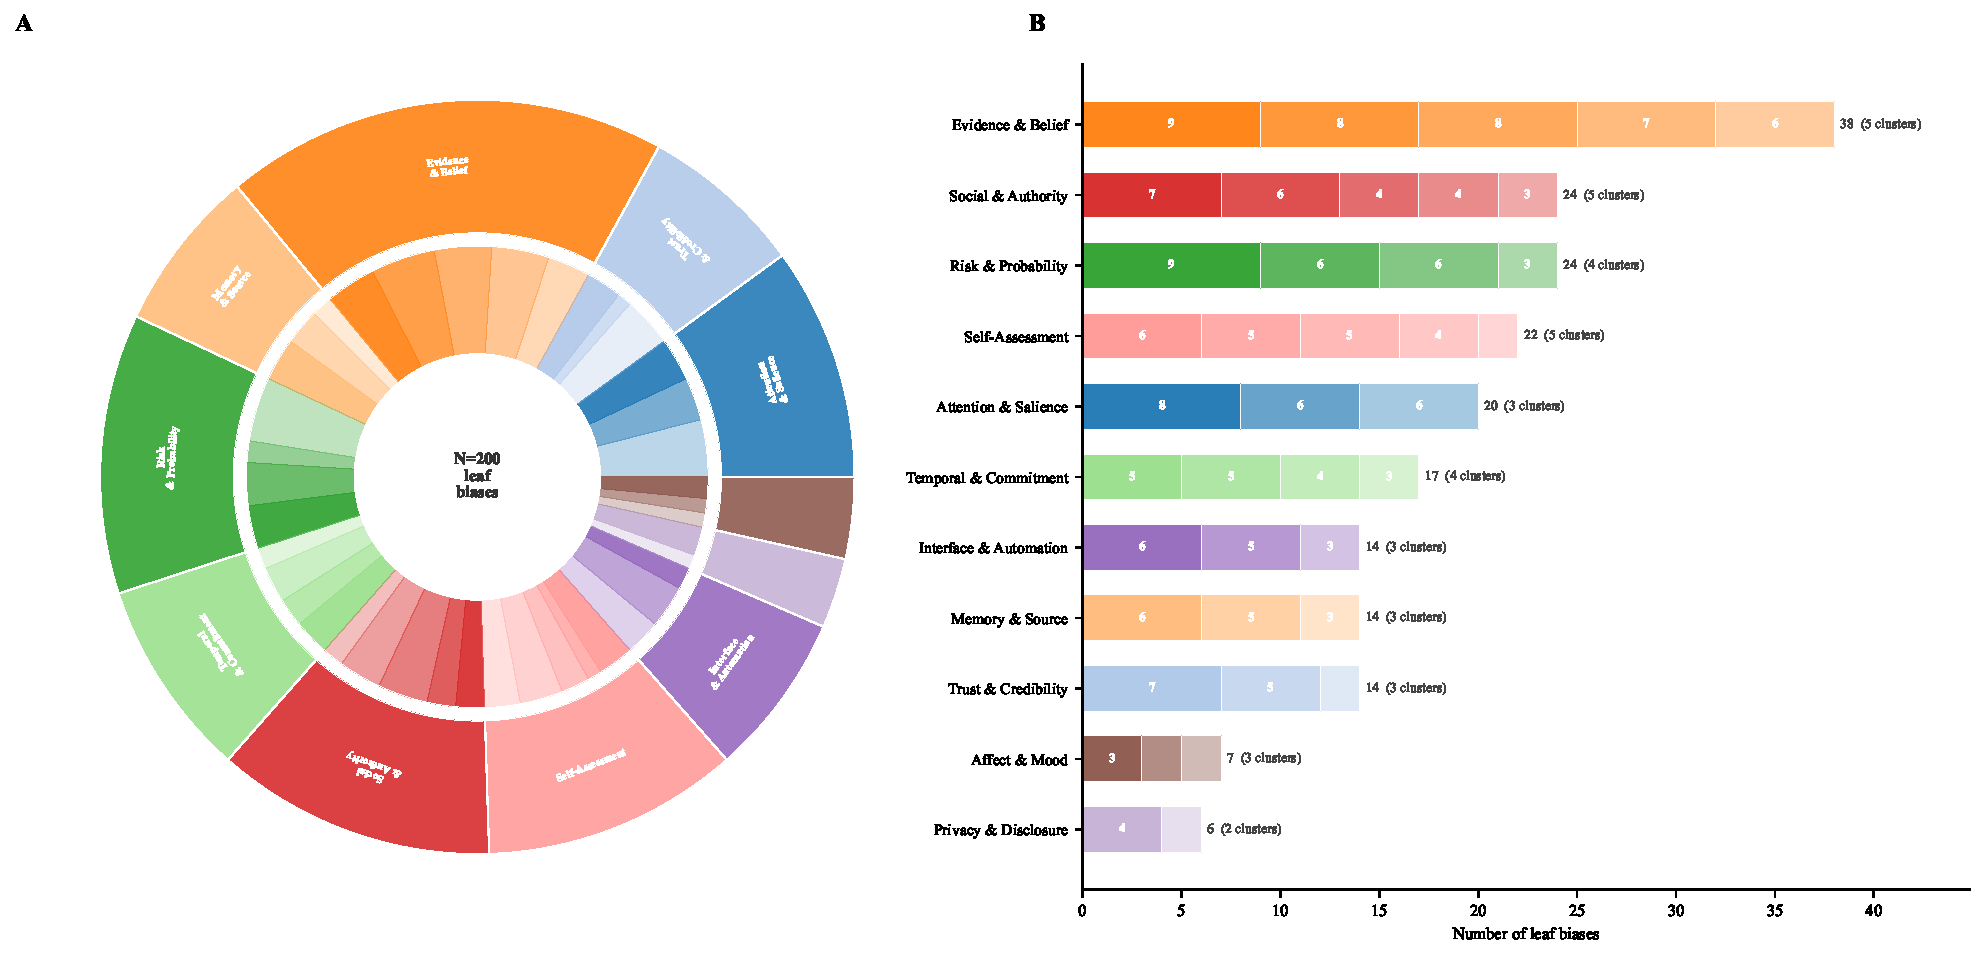
\includegraphics[width=0.92\textwidth]{../assets/figures/fig1_taxonomy_sunburst.pdf}
  \fignote{The frozen taxonomy contains 200 cognitive biases in 40 clusters across 11 top-level families. Segment area reflects leaf-bias count. Full counts and mean \ecbss{} values per family are in Supplementary Table~\ref{tab:s1-taxonomy}; the complete inventory is in Supplementary Table~\ref{tab:s6-taxonomy}.}
\end{figure}

\subsection{Emotion Space and Cluster Profiles}

$k$-means clustering partitioned the 239-emotion lexicon into six groups with interpretable affective profiles: Hostile \& Defiant ($n = 16$), Alarmed \& Uncertain ($n = 66$), Socially Vulnerable ($n = 47$), Withdrawn \& Low Arousal ($n = 34$), High-Arousal Positive ($n = 37$), and Calm Positive ($n = 39$) (Figure~\ref{fig:landscape}; Supplementary Tables~\ref{tab:s4-cluster} and~\ref{tab:s5-clusters}). The $k = 6$ solution yielded a silhouette score of 0.365; silhouette peaked at $k = 8$ (0.407), but $k = 6$ was retained for interpretability and profile distinctness. Within-cluster coherence was confirmed visually in both the UMAP projection \citep{mcinnes2018umap} (Figure~\ref{fig:landscape}) and the PCA biplot (Supplementary Figure~\ref{fig:s4}).

The Hostile \& Defiant cluster combined strongly negative valence, high arousal, high perceived control, and strongly antisocial orientation---an active, outward-directed antagonistic profile. The Alarmed \& Uncertain cluster was defined by negative valence, high arousal, low perceived control, and high uncertainty---a signature of acute threat without coping resources, directly relevant to phishing and urgency-based social engineering. The Socially Vulnerable cluster showed moderate negative valence, moderate arousal, and high prosocial orientation, capturing shame, embarrassment, and longing. Withdrawn \& Low Arousal states combined negative valence with low arousal and moderate certainty. High-Arousal Positive states showed high valence, high arousal, high control, and moderate prosociality (e.g., excitement, enthusiasm, elation). Calm Positive states showed positive valence with low-to-moderate arousal and higher certainty.

\begin{figure}[tb]
  \raggedright
  \caption{Emotion landscape in affective component space}
  \label{fig:landscape}
  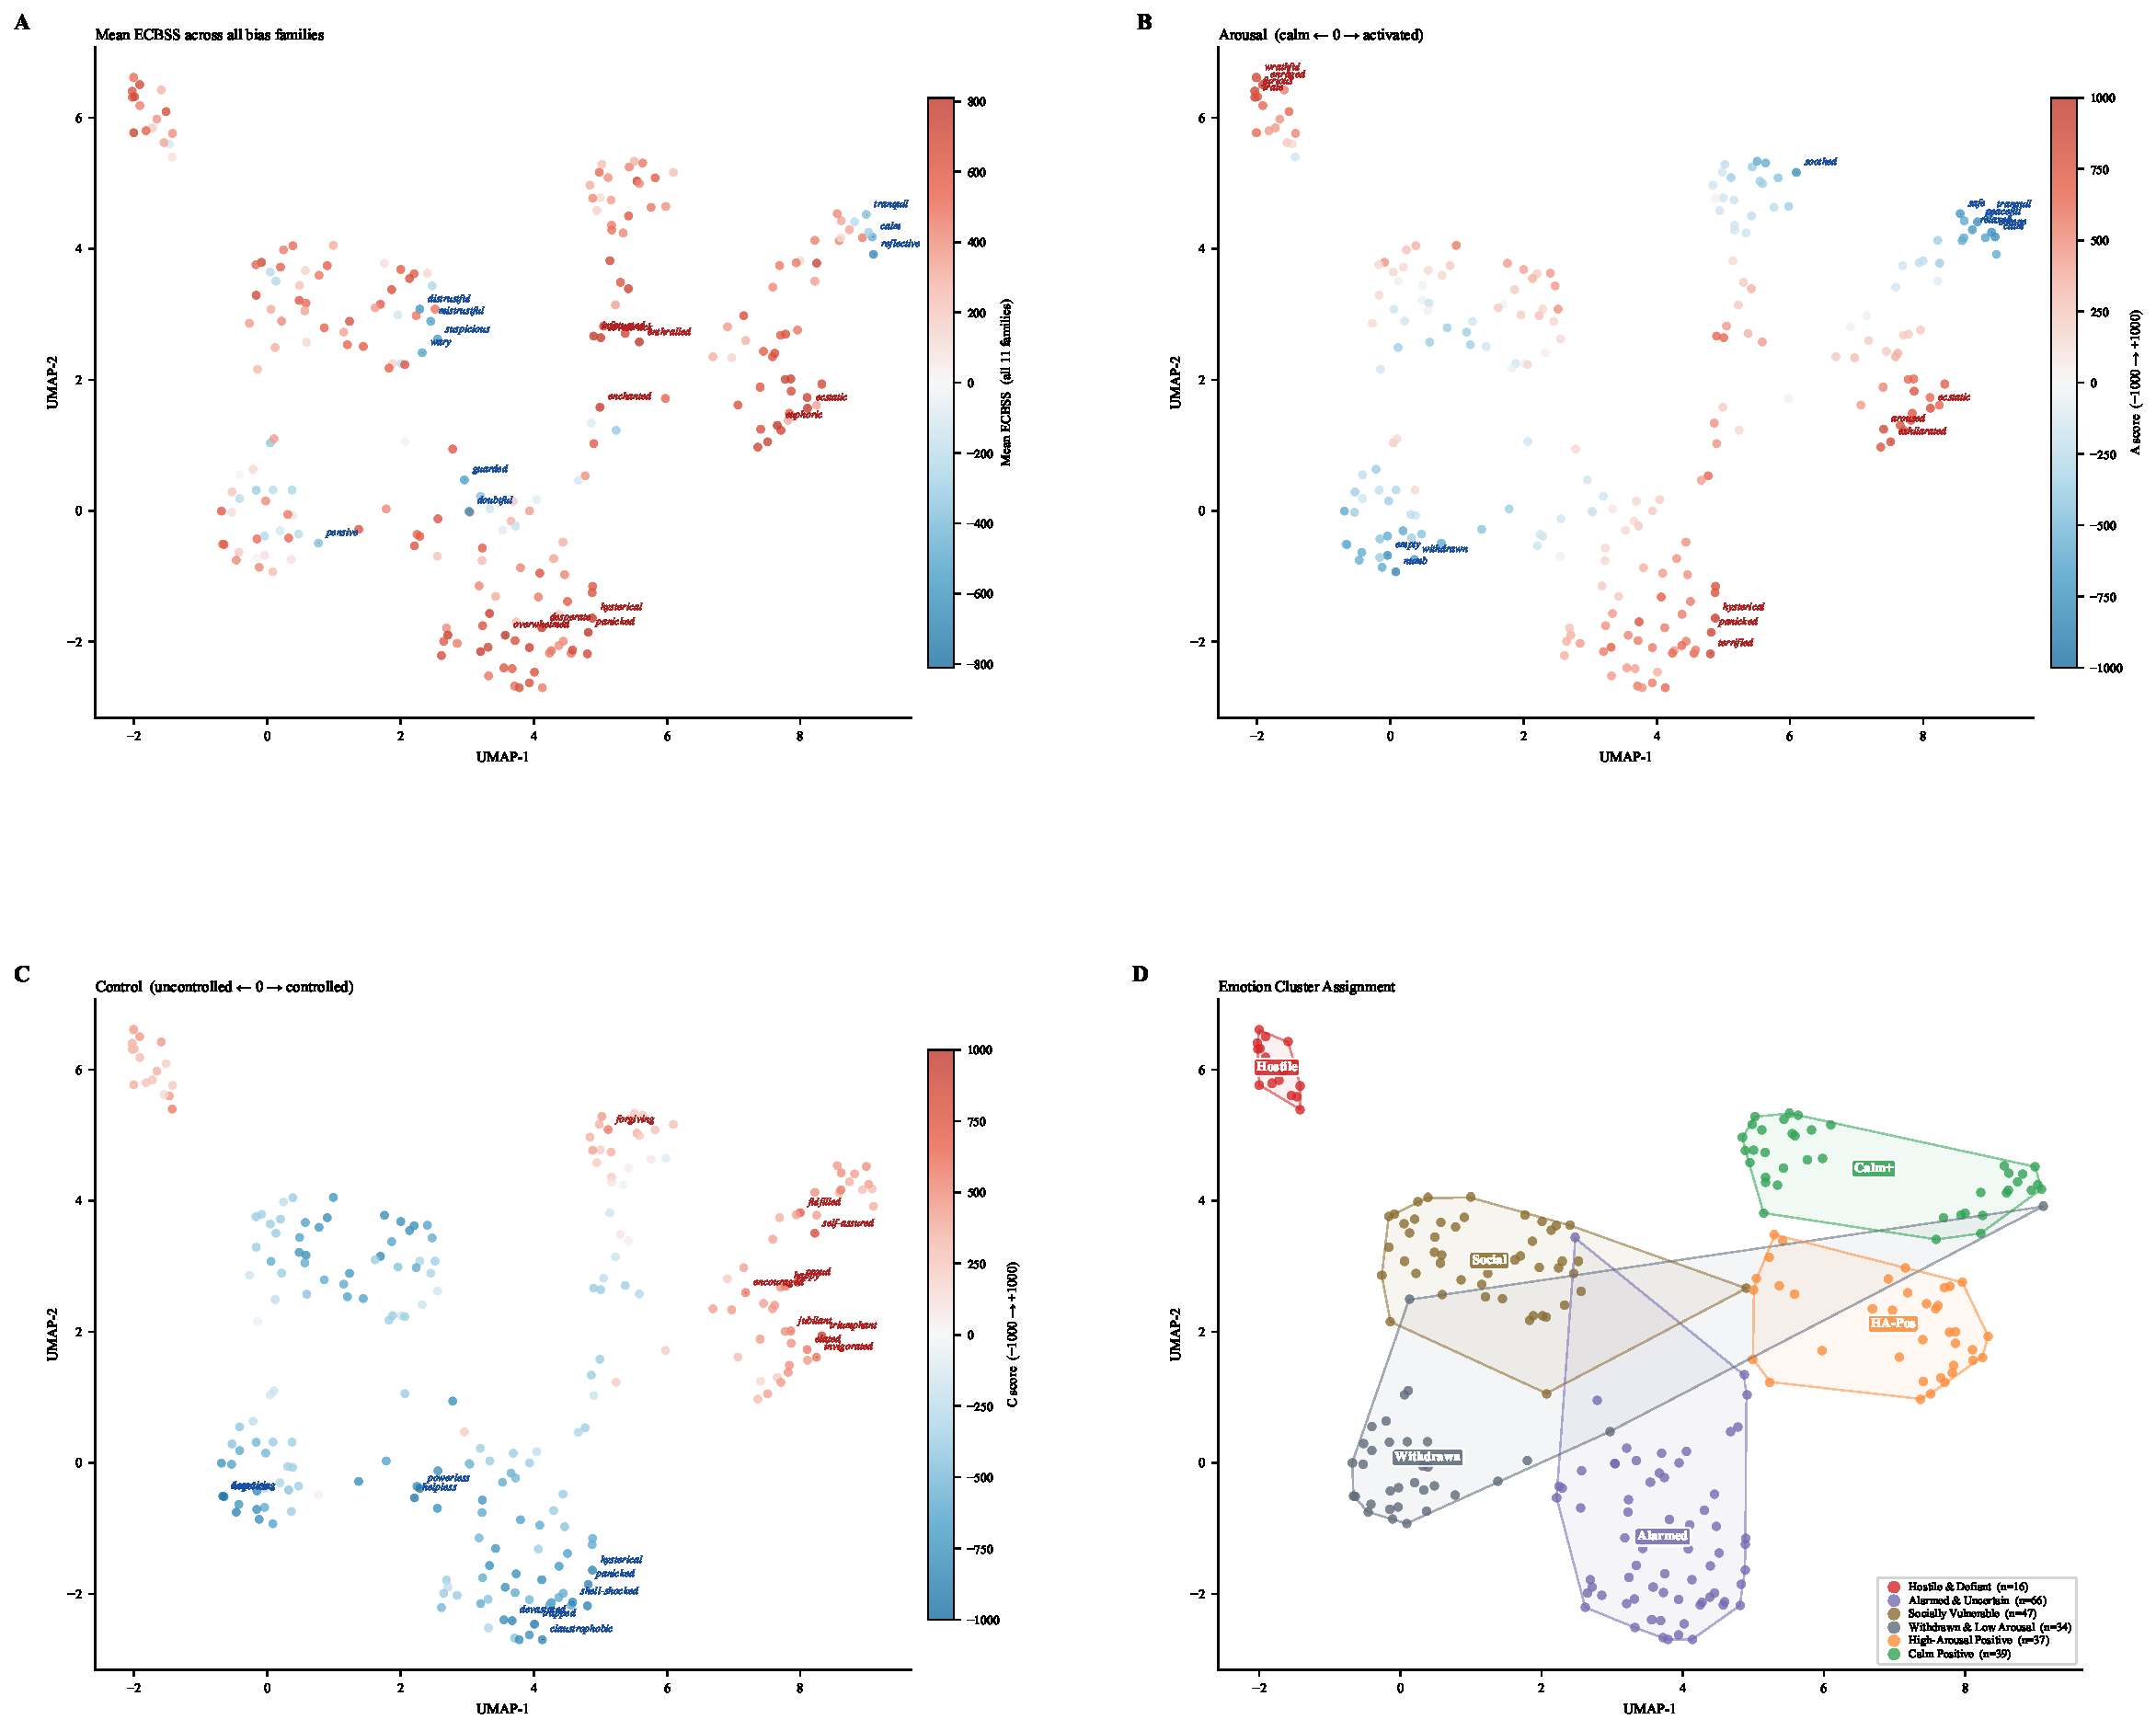
\includegraphics[width=\textwidth]{../assets/figures/fig2_emotion_landscape.pdf}
  \fignote{UMAP projection of the 239-emotion lexicon colored by cluster membership. UMAP parameters: $n_{\mathrm{neighbors}} = 20$, $\mathrm{min\_dist} = 0.3$. The projection is used for visualization only; primary inference is based on the original five-dimensional \vacus{} space. Full cluster profiles with centroid-nearest representative emotions are in Supplementary Table~\ref{tab:s5-clusters}.}
\end{figure}

\subsection{ECBSS Distribution and RQ1}

Across the full $239 \times 11$ matrix, the grand mean \ecbss{} was 368.8 ($SD = 472.8$, median $= 450.0$; Supplementary Figure~\ref{fig:s2}), with 77.6\% of cells positive (amplifying) and 22.4\% negative (attenuating), directly answering \textbf{RQ1}: emotional states do systematically shift bias vulnerability, and the dominant direction is amplification. The distribution was left-skewed relative to the +1000 ceiling: amplifying scores concentrated in the 300--800 range, while attenuation scores were mostly in the 0 to $-400$ range with a tail below $-700$. This asymmetry indicates a general amplification bias with selective, context-specific attenuation---not a symmetric bidirectional pattern.

The most extreme amplifying cell was \textit{hysterical} paired with affect and mood biases (\ecbss{} $= +985$). The strongest attenuation involved distrust- and contempt-related states paired with social-influence and trust families (\ecbss{} $\leq -800$; Supplementary Table~\ref{tab:s2-pairs}). Cluster-level means ranged from 111.5 (Withdrawn \& Low Arousal) to 581.8 (High-Arousal Positive), confirming that the specific emotional context of a cyber interaction substantially shapes which vulnerability profile is active.

\begin{figure}[tb]
  \raggedright
  \caption{Cluster-by-family mean \ecbss{} heatmap}
  \label{fig:heatmap}
  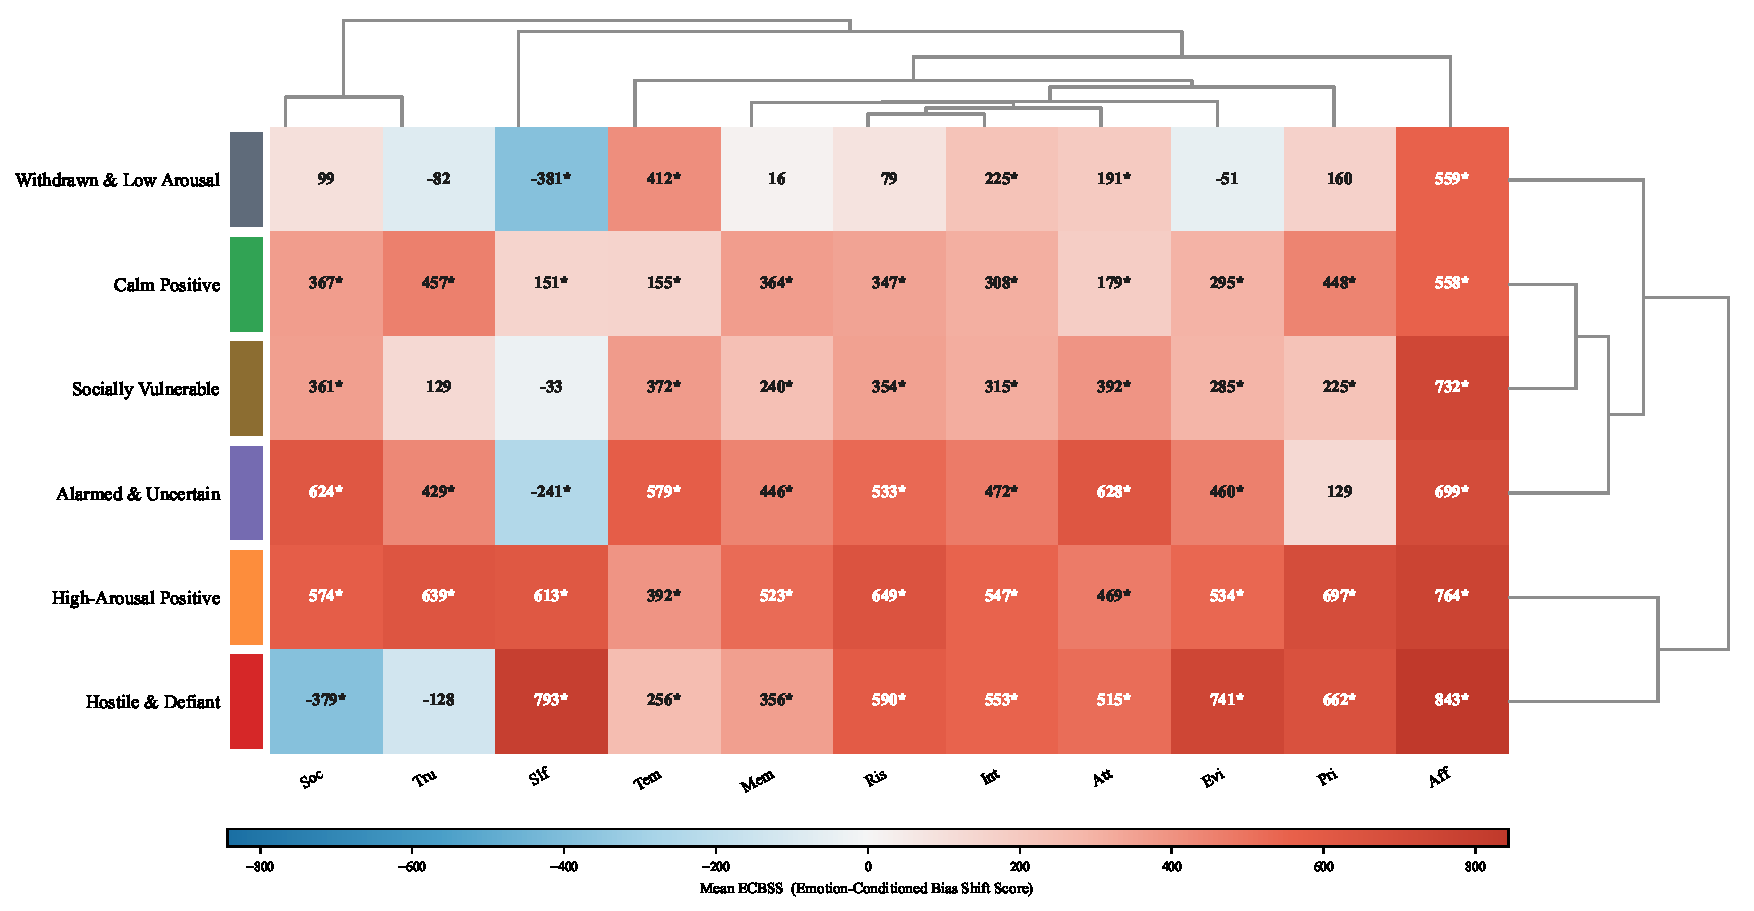
\includegraphics[width=\textwidth]{../assets/figures/fig3_ecbss_heatmap.pdf}
  \fignote{Mean \ecbss{} for each of the six emotion clusters (rows) and 11 bias families (columns). Both margins are hierarchically clustered to expose similarity structure. Asterisks mark cells whose 1,000-resample bootstrap interval excludes zero. Red cells indicate amplification; blue cells indicate attenuation relative to neutral. Numeric values are in Supplementary Table~\ref{tab:s4-cluster}.}
\end{figure}

\subsection{Component Drivers of Vulnerability and RQ2 and RQ4}

The mixed-effects regression (Equation~\ref{eq:mixedeffects}) identified four of the five affective components as significant predictors, answering \textbf{RQ2} (Table~\ref{tab:mixed_effects}). Arousal was the strongest global amplifier ($\beta = 504.1$, $SE = 20.8$, $p < .001$): independent of which family is targeted, higher activation is associated with approximately half a scale unit of additional vulnerability. Control/coping was the strongest attenuator ($\beta = -542.3$, $SE = 32.0$, $p < .001$). Valence was positively associated with \ecbss{} ($\beta = 275.1$, $SE = 19.5$, $p < .001$), meaning more positive emotional states also tend toward amplification---challenging the heuristic that negative emotion is the primary driver of cyber vulnerability. Uncertainty showed a significant \textit{attenuating} effect ($\beta = -357.1$, $SE = 22.6$, $p < .001$), counter to the directional expectation. Social orientation was not significant ($\beta = -1.6$, $SE = 17.4$, $p = .925$). Regarding \textbf{RQ4}, the random-intercept variance was significantly non-zero ($\hat{\tau}^2 = 0.118$, $p = .024$), confirming that affective components explain a meaningful but incomplete share of variance, with additional family-level baseline differences beyond fixed effects.

\begin{table}[tb]
  \raggedright
  \small
  \caption{Mixed-effects regression of \ecbss{} on affective components}
  \label{tab:mixed_effects}
  \resizebox{\textwidth}{!}{%
  \setlength{\tabcolsep}{9pt}%
  \begin{tabular}{@{}lrrrrl@{}}
    \toprule
    Predictor & $\beta$ & $SE$ & $p$ & Perm.\ $p$ & 95\% CI \\
    \midrule
    Intercept                 & $+220.1$ & 43.0 & $<.001$ & ---     & $[+135.9,\ +304.3]$ \\
    Valence (V)               & $+275.1$ & 19.5 & $<.001$ & $<.001$ & $[+236.9,\ +313.3]$ \\
    Arousal (A)               & $+504.1$ & 20.8 & $<.001$ & $<.001$ & $[+463.3,\ +544.9]$ \\
    Control (C)               & $-542.3$ & 32.0 & $<.001$ & $<.001$ & $[-605.0,\ -479.6]$ \\
    Uncertainty (U)           & $-357.1$ & 22.6 & $<.001$ & $<.001$ & $[-401.4,\ -312.8]$ \\
    Social orientation (S)    & $-1.6$   & 17.4 & $.925$  & $.930$  & $[-35.8,\ \ +32.6]$  \\
    \midrule
    Random intercept (family) & \multicolumn{5}{l}{$\hat{\tau}^2 = 0.118$,\; $p = .024$} \\
    \bottomrule
  \end{tabular}%
  }
  \tabnote{$N = 2{,}629$ emotion-family observations with 11 families in random effects. 95\% CI computed as $\beta \pm 1.96 \times SE$. Permutation $p$-values are from 1,000 label-permuted null distributions with OLS refitting at each permutation. Per-family OLS coefficients and $R^2$ are in Supplementary Table~\ref{tab:s3-regression}.}
\end{table}

All four significant effects survived permutation tests (each at $p < .001$ over 1,000 permutations; zero permuted coefficients exceeded the observed magnitude). Social orientation failed permutation consistently ($p = .930$). Per-family $R^2$ values ranged from .232 (privacy and disclosure) to .497 (self-assessment and metacognitive biases): component structure accounted for most variance in introspective families (self-assessment: $R^2 = .497$; social influence: $.426$; trust: $.381$) but less in situationally specific families (interface and warning response: $.249$; privacy: $.232$). This confirms that for \textbf{RQ4}, the component-based account outperforms a null model throughout, but explained variance remains family-dependent.

Family-level sensitivity profiles and coefficient diagnostics are reported in Supplementary Figure~\ref{fig:s9}.

\subsection{Cluster-Level Profiles and RQ3}

Addressing \textbf{RQ3}, the six emotion clusters produced qualitatively distinct vulnerability profiles (Figure~\ref{fig:heatmap}; Supplementary Table~\ref{tab:s4-cluster}). The High-Arousal Positive cluster (cluster~4, $n = 37$, mean $= 581.8$) showed broad amplification across all 11 families without exception, including self-assessment ($+613$), trust ($+639$), social influence ($+574$), and privacy disclosure ($+697$). The Hostile \& Defiant cluster (cluster~0, $n = 16$, mean $= 436.6$) combined extreme amplification of affect and mood ($+843$), self-assessment ($+793$), and evidence processing ($+741$) with the only supra-threshold attenuation in the matrix: social influence ($-379$) and, below the visualization threshold, trust ($-128$). The Alarmed \& Uncertain cluster (cluster~1, $n = 66$, mean $= 432.7$) strongly amplified attention ($+628$), social influence ($+625$), and temporal biases ($+579$) but suppressed self-assessment ($-241$). The Withdrawn \& Low Arousal cluster (cluster~3, $n = 34$, mean $= 111.5$) showed the lowest overall amplification, with notable attenuation of self-assessment ($-382$) and, below threshold, trust ($-82$) and evidence processing ($-52$).

Bootstrap confidence intervals excluded zero for 56 of 66 cluster-by-family cells (84.8\%), confirming stability of the cell-level patterns under resampling. Cohen's $d$ for high-arousal fear states (afraid, panicked, alarmed, terrified, horrified) versus calm baseline states on the social influence family was 3.605 ($t(8) = 5.70$, $p = .004$), illustrating the practical magnitude of the arousal effect on the family most directly implicated in phishing and authority-based social engineering.

\subsection{Variance Structure, Factor Analysis, and Network}

Variance decomposition confirmed that emotion cluster and bias family contributed similar shares of total \ecbss{} variance ($\eta^2_{\text{cluster}} = .093$, $F(5, 2613) = 53.4$, $p < .001$; $\eta^2_{\text{family}} = .097$, $F(10, 2613) = 28.0$, $p < .001$; Supplementary Figure~\ref{fig:s9}, Panel~D; Supplementary Table~\ref{tab:s4-cluster}). Crucially, 81.0\% of total variance resided in pair-specific residuals, confirming that coarse cluster membership and coarse family labels each explain roughly 10\% of variance and that the remaining 80\% reflects unique emotion-by-family interactions.

Factor analysis of the $11 \times 11$ family correlation matrix ($N_{\text{obs}} = 239$) recovered three factors (Supplementary Figure~\ref{fig:s9}, Panels~B--C). Factor~1 loaded on interface and warning-response ($-0.72$), attention ($-0.66$), and risk and probability ($-0.64$): families characterized by heightened responsiveness to environmental signal salience. Factor~2 loaded on self-assessment ($-0.96$), memory and source-monitoring ($-0.71$), and privacy ($-0.52$): introspective and metacognitive families sensitive to internal confidence. Factor~3 loaded on evidence processing ($+0.80$), social influence ($+0.75$), temporal choice ($+0.71$), and trust ($+0.68$): families engaged in social-inferential and information-credibility evaluation. This three-factor structure provides a principled reduction of the 11-family space for targeting interventions (see Section~\ref{sec:discussion-factor}).

The bipartite cluster-to-family network (Figure~\ref{fig:network}) summarizes both mean-link strength and link-level dispersion. Across all 66 possible cluster-family pairs, amplification links dominate the global structure, with attenuation concentrated in specific cluster-family combinations (notably social-influence and self-assessment nodes under high-skepticism or depleted states). The network remained connected in coefficient space, and connector families such as trust and privacy retained high betweenness, indicating that these domains bridge otherwise distinct cluster vulnerability profiles.

\begin{figure}[tb]
  \raggedright
  \caption{Bipartite network of emotion clusters and bias families}
  \label{fig:network}
  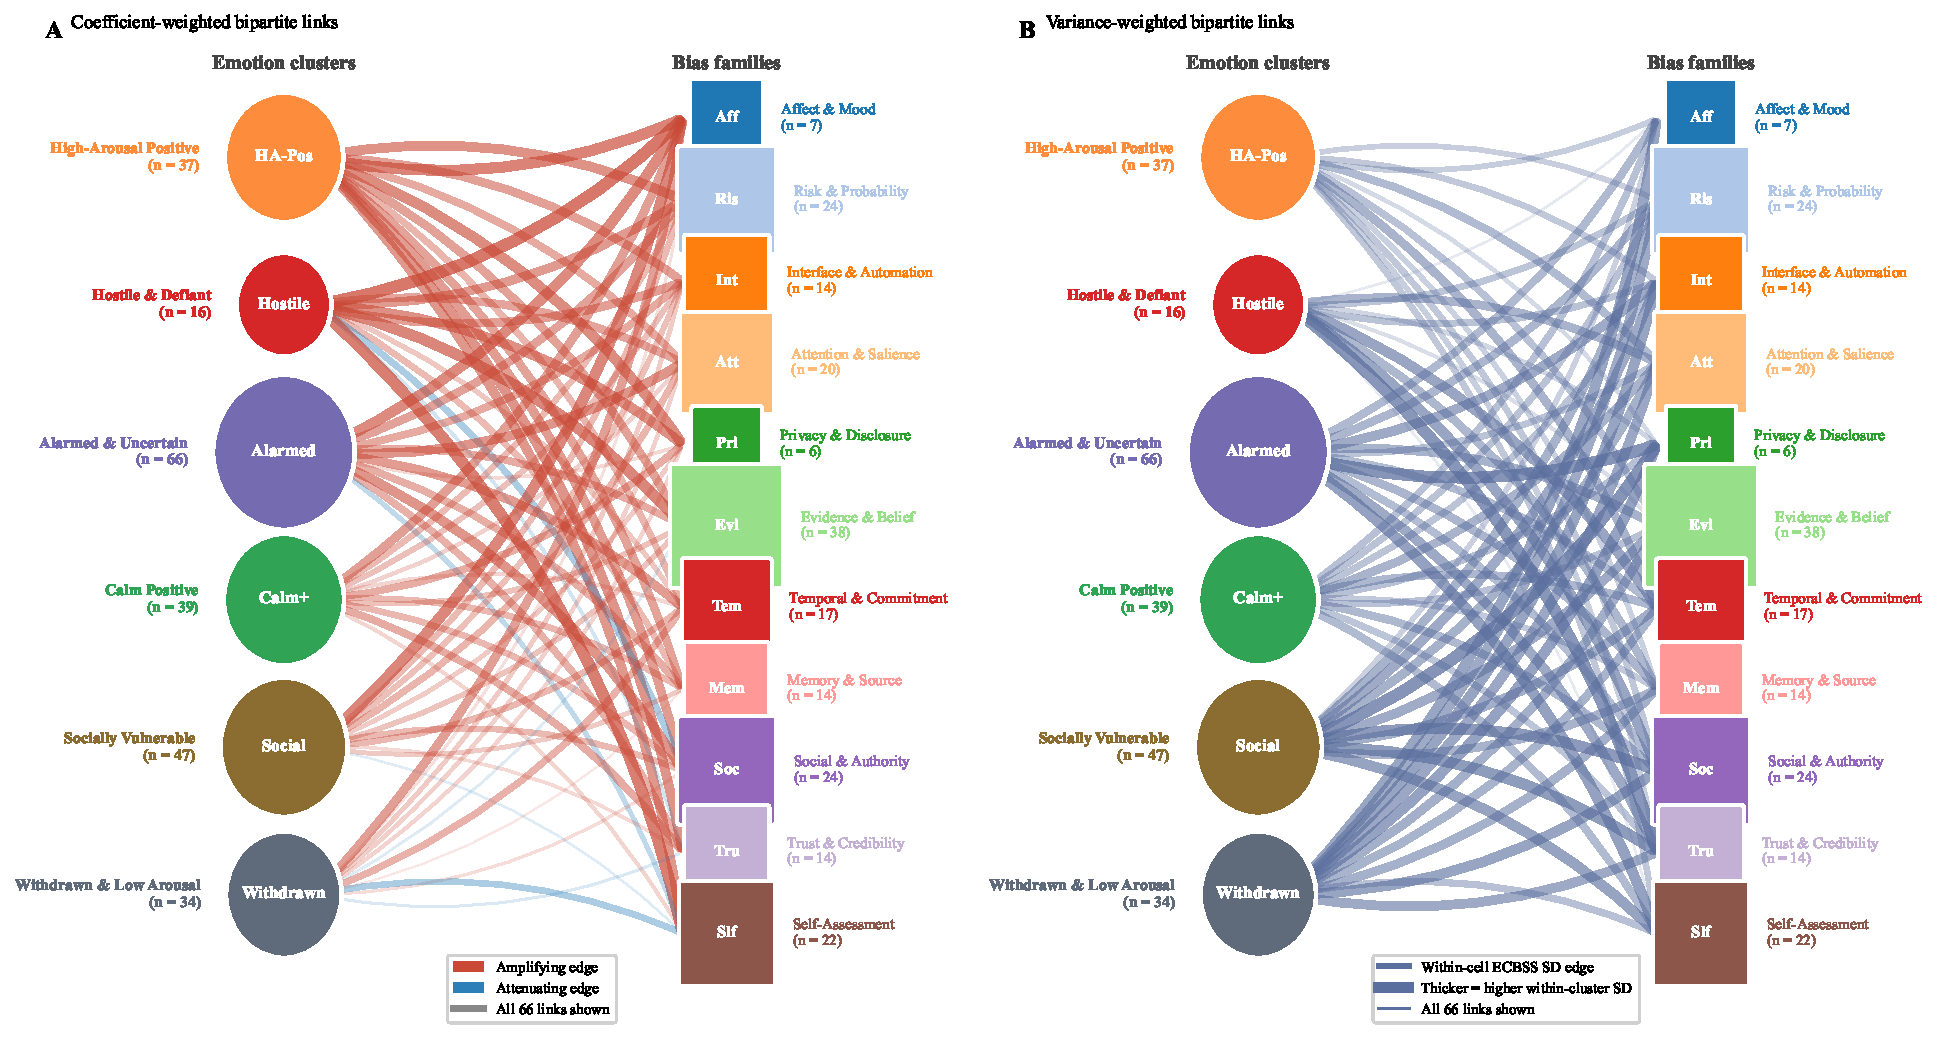
\includegraphics[width=\textwidth]{../assets/figures/fig5_network.pdf}
  \fignote{Panel A shows the coefficient-weighted bipartite structure linking emotion clusters (left) to bias families (right). Panel B shows variance-weighted links for the same topology, capturing within-cell dispersion rather than mean direction alone. Red edges indicate amplification-dominant effects and blue edges attenuation-dominant effects.}
\end{figure}

\subsection{Analytical--Direct Score Convergence}

The Pearson correlation between the analytical benchmark (Equation~\ref{eq:analytical}) and the direct \ecbss{} scores was $r = .324$ ($p < .001$; Spearman $\rho = .372$, $p < .001$; $N = 2{,}629$). The ICC between methods was low (ICC$(2,1) = 0.188$, 95\% CI $[.161, .216]$; ICC$(3,1) = 0.266$, 95\% CI $[.231, .302]$), indicating substantial systematic method variance. Convergence was strongest for self-assessment ($r = .608$) and weakest for interface and warning-response ($r = .094$, $p = .149$, non-significant). The divergence in interface families suggests that direct scoring captured interaction-specific nuances (e.g., automation bias and alert-fatigue dynamics) that were not fully represented by the additive component benchmark (Supplementary Figure~\ref{fig:s7}, Panel~B).

Detailed regression structure and family-level variance-explained diagnostics are reported in Supplementary Figure~\ref{fig:s9} (Panels B--D).

%% ============================================================
\section{Discussion}
%% ============================================================

\subsection{Arousal as the Primary Amplifier of Cyber Vulnerability}

The dominant result---arousal as the strongest positive predictor ($\beta = 504.1$, permutation $p < .001$) of vulnerability across all 11 bias families---is consistent with two complementary theoretical accounts. The risk-as-feelings model \citep{loewenstein2001risk} predicts that physiological arousal generates visceral reactions that override deliberate evaluation, shifting the decision-maker toward the fast heuristic path. The affect heuristic \citep{slovic2007affect} specifies the mechanism: arousal increases the weight of affective tags on incoming stimuli relative to analytical risk estimates. In the context of phishing and social engineering, this translates directly to a measurable vulnerability window: any manipulation that elevates user arousal---whether through countdown timers, simulated account alerts, urgency language, or personalized threat cues---should be expected to amplify susceptibility across the full range of cyber-relevant bias families, not merely those that are overtly affective.

Crucially, the amplification is direction-agnostic: both fearful high-arousal states (Alarmed \& Uncertain, mean $= 432.7$) and excited positive high-arousal states (High-Arousal Positive, mean $= 581.8$) showed strong amplification. The High-Arousal Positive cluster was in fact the most uniformly vulnerable profile in the entire matrix, including self-assessment ($+613$) and trust ($+639$). This finding is consistent with the broaden-and-build account \citep{fredrickson2001positive}: positive arousal may broaden attentional scope and increase receptivity to new information, a state of exploratory openness that becomes a security liability when the new information includes deceptive cues. Security awareness programs that induce celebratory states at the moment of a decision---by, for example, delivering a gamified reward (e.g., points, a badge, or a level-up animation) immediately after a correct threat-identification decision---may inadvertently place users in the most vulnerable zone of the cognitive bias vulnerability map at the subsequent affective interaction.

\newpage
\subsection{Perceived Control as the Primary Protective Factor}

The control/coping coefficient ($\beta = -542.3$) is the largest single effect in the model and carries a clear translational message. Perceived coping capacity---the sense that one has sufficient resources to manage the situation---is the foundational construct of stress-and-coping theory \citep{lazarus1984stress}. High perceived control is associated with problem-focused, deliberate processing rather than emotion-focused heuristic shortcuts; it is the affective component most directly linked to the deliberate System~2 processing that \citet{kahneman2011thinking} and \citet{evans2008dual} identify as the protective counterweight to heuristic vulnerabilities.

The practical implication is concrete: interface designs, notification formats, and operational contexts that preserve user agency and reduce helplessness should attenuate bias vulnerability. Conversely, designs that create time pressure, remove decision options, or emphasize the user's inability to change the situation (e.g., ``your account will be suspended unless you act now'') directly erode perceived control and therefore directly increase the vulnerability window. The ``controlled skepticism'' pattern of the Hostile \& Defiant cluster---strong attenuation of social influence ($-379$) and trust alongside amplification of self-assessment and evidence biases---demonstrates this principle from the other direction: when perceived control is very high in a context of negative social affect, interpersonal compliance cues are actively suppressed, even at the cost of amplifying internally directed cognitive errors.

\subsection{Uncertainty as Component Attenuator: Cautious Processing}

The significant attenuating effect of uncertainty ($\beta = -357.1$, permutation $p < .001$) was not predicted a priori and runs counter to the classical finding that ambiguity increases reliance on heuristics \citep{tversky1974judgment, kahneman2011thinking}. Two non-mutually-exclusive interpretations merit empirical follow-up. First, high uncertainty may activate a cautious, exploratory mode in which the perceiver explicitly acknowledges not knowing the correct answer; this metacognitive signal of insufficient information may inhibit confident heuristic responding---``I don't know, so I should be careful''---rather than promoting it through increased schema reliance. Second, the \vacus{} uncertainty component in this study reflects perceived situational ambiguity rather than statistical uncertainty about an outcome; situational ambiguity may promote heightened attention to incoming cues \citep{lerner2015emotion}, which could serve as an error-detection mechanism. Distinguishing these accounts requires targeted experimental designs with separate manipulations of objective and subjective uncertainty.

\subsection{Cluster-Specific Profiles and Intervention Implications}

\label{sec:discussion-factor}

The qualitatively distinct cluster profiles established in \textbf{RQ3} have different implications for security intervention design. The three-factor structure recovered in the factor analysis (Supplementary Figure~\ref{fig:s9}, Panels~B--C) provides a useful organizing principle: (1) \textit{situationally responsive families} (Factor~1: interface, attention, risk)---most effectively targeted by interface-level modifications that reduce cue salience and insert processing friction; (2) \textit{introspective/metacognitive families} (Factor~2: self-assessment, memory, privacy)---more effectively addressed through training that enhances self-monitoring capacity, since their susceptibility is driven by internal confidence evaluations; and (3) \textit{social-inferential families} (Factor~3: evidence, social influence, temporal, trust)---most directly implicated in social engineering and benefiting from protocols that slow authority evaluation and source-credibility checking.

The Hostile \& Defiant cluster exemplifies the ``controlled skepticism'' pattern: very high amplification of self-assessment and evidence biases combined with strong attenuation of social influence. A user in a hostile or contemptuous state may be less susceptible to authority-based phishing (attenuated social influence) but more prone to overconfident attribution and confirmation-seeking errors. Interventions that attempt to build security resilience through anger-based framing \citep{lerner2000beyond}---for example, showing users past phishing attempts and framing them as attacks to resist---risk trading social-influence susceptibility for overconfidence in the user's own security judgment.

\subsection{Scientific and Practical Value of the Synthetic Scoring Approach}

The use of LLM-based synthetic scoring at scale offers several advantages that empirical laboratory designs cannot readily match. First, the 2,629-cell emotion-by-family matrix would require recruiting thousands of participants across highly diverse emotional states to replicate behaviorally---most states (e.g., \textit{hysterical}, \textit{awestruck}) are difficult or ethically problematic to induce in laboratory settings. The synthetic-scoring approach provides full coverage at marginal cost. Second, privacy regulations and ethics constraints substantially limit the collection, storage, and processing of affect data in the human participant research context; the synthetic-scoring approach bypasses these constraints entirely, enabling large-scale population-level modeling without sensitive personal data. Third, deterministic zero-temperature scoring produces a stable, reproducible matrix that can serve as a benchmark: human behavioral data, when available, can be compared against this baseline to identify domains where the model diverges from observed behavior, providing direct targets for model refinement. Fourth, the output is already structured as a decision matrix, enabling direct computational integration into adaptive security systems that could, in principle, adjust friction levels or alert formats based on inferred emotional state.

A growing body of methodological work validates the use of LLM-generated synthetic data as a complement or precursor to human behavioral studies. \citet{argyle2023out} demonstrate that language models can accurately reproduce the distribution of attitudes across demographic strata in large-scale survey samples. \citet{grossmann2023ai} identify structured LLM elicitation as a principled method for social-science hypothesis generation. More recently, \citet{ziems2024can} show that LLM annotations achieve near-human interrater reliability on complex psychological rating tasks. The Stanford HAI policy brief \citep{santurkar2023opinions} further demonstrates that AI agent ensembles can replicate attitude distributions at scale. Collectively, these results support the inferential value of LLM-elicited synthetic scores as a principled first-pass mapping that identifies promising targets for human behavioral follow-up.

\subsection{Limitations}
\label{sec:limitations}

Five substantive limitations constrain the inferential scope of the present results.

Single-model implementation. Scores were generated by a single LLM (\textit{google/gemini-3-flash-preview}), and the low ICC between direct and analytical scores (ICC$(2,1) = 0.188$) reveals substantial systematic method variance between the two scoring approaches. Whether this divergence reflects genuine contextual reasoning in direct scores or model-specific response bias cannot be determined from the present data. Practically, this means that cells where the model assigns extreme \ecbss{} values may partly reflect idiosyncratic response tendencies of the scoring model rather than theoretically grounded sensitivity. An ensemble design---replicating the scoring protocol across architecturally distinct models and computing ICC profiles across families---would separate stable, theory-consistent signal from model-specific artifacts.

Family-level aggregation. The scoring matrix was computed at the bias-family level, aggregating 12--25 cognitive biases per family. Within-family heterogeneity---which the factor analysis suggests is substantial---is therefore not captured in the present estimates. That said, family-level granularity was sufficient to address the current research questions, which concern differential vulnerability profiles across broad cognitive processing domains rather than the internal structure of individual bias families.

Theory-saturated synthetic scores. The \ecbss{} values generated by \textit{google/gemini-3-flash-preview} represent the model's internalized theoretical knowledge about emotion--cognition relationships rather than sampled human behavior. Crucially, this means the study samples a theory-compressed representation of how the model construes human psychology, not a sample from the population of human decision-makers. This distinction is not merely semantic: if the model's internal representations systematically overweight or underweight particular emotion--bias associations relative to the ground truth of human behavior, the resulting \ecbss{} matrix will propagate those biases at scale. The large effect magnitudes observed---coefficients of $\pm 500$ on a $\pm 1000$ scale---should accordingly be interpreted as reflecting the internal geometry of the model's response space rather than as estimates of behavioral effect sizes in human populations.

An emerging methodological literature cautions that LLMs exhibit performance inconsistency, prompt brittleness, and memorisation artifacts that limit their validity as behavioural surrogates \citep{gao2025llm, dillion2023ai}. These concerns are most acute when outputs are treated as calibrated estimates of human behavioural frequencies; the present use is more circumscribed, treating \ecbss{} scores as a theoretically structured prior for organising the hypothesis space rather than as substitutes for human participant data.

Linear modeling assumption. The inferential pipeline relies entirely on linear and parametric methods (mixed-effects regression, two-way ANOVA, factor analysis). Non-linear approaches---such as gradient boosted trees, random forests, kernel-based models, or deep learning architectures---may better capture interaction and threshold effects between affective components, potentially explaining a portion of the 81\% of variance currently residing in pair-specific residuals.

\newpage
\subsection{Future Directions}

Several high-priority extensions follow from the present results. First, the uncertainty paradox warrants targeted replication with human participants under independent manipulations of objective ambiguity and subjective uncertainty. Second, the leaf-level scoring matrix---all 200 cognitive biases $\times$ 239 emotions---would resolve the within-family heterogeneity identified by the factor analysis and provide a finer-grained intervention target. Third, ecological-validity testing is now essential: predicted high- and low-vulnerability emotion-family pairs should be evaluated in behavioral experiments and in observational data settings (e.g., social-media-adjacent cyber-warning responses or field phishing simulations) to test external validity. Fourth, the cluster-level profile differences---particularly controlled-skepticism and withdrawn-protection patterns---suggest that emotion-aware, context-adaptive training may outperform generic awareness programs. Fifth, ecological validity testing in naturalistic digital environments---including field analysis of social-media-adjacent cyber-warning response data, red-team cyber-range experiments \citep{beltz2025gambit}, and experience-sampling studies of emotion and security decision-making in organizational settings---is necessary to establish whether the theoretically derived vulnerability map generalizes to real human populations under authentic digital conditions. Sixth, content-based multi-modal risk estimation---combining textual, visual, and behavioural signals to infer affective state and predict cognitive-bias vulnerability in real time---represents a high-priority applied extension of the present framework, enabling targeted, affect-sensitive counter-nudge interventions for active cybersafety protection.

%% ============================================================
\section{Conclusion}
%% ============================================================

This study provides the first large-scale, dimensionally structured characterisation of how discrete emotional states modulate cognitive-bias susceptibility across a comprehensive taxonomy of cyber-relevant decision contexts. The central finding---that vulnerability is organised primarily by physiological activation and perceived coping capacity, with arousal as the dominant amplifier ($\beta = 504.1$) and control as the dominant attenuator ($\beta = -542.3$) across all 11 bias families---reframes valence-focused accounts of affective risk and carries direct implications for security interface design, adaptive training, and emotion-aware detection systems. The counterintuitive attenuation by uncertainty and the 81\% pair-specific residual variance jointly establish that coarse emotional category membership cannot substitute for fine-grained affective profiling. The taxonomy, scored emotion lexicon, and complete \ecbss{} matrix are made available as open research infrastructure to support behavioural replication, multi-model validation, and leaf-level extension across the full cognitive-bias space.

\clearpage
\bibliographystyle{apalike}
\bibliography{other/references}

\clearpage
\setcounter{figure}{0}
\renewcommand{\thefigure}{S\arabic{figure}}
\setcounter{table}{0}
\renewcommand{\thetable}{S\arabic{table}}

\section*{Supplementary Materials}

\subsection*{Supplementary Figures}

\begin{figure}[!htb]
  \raggedright
  \caption{PRISMA-informed review workflow for taxonomy curation}
  \label{fig:s1}
  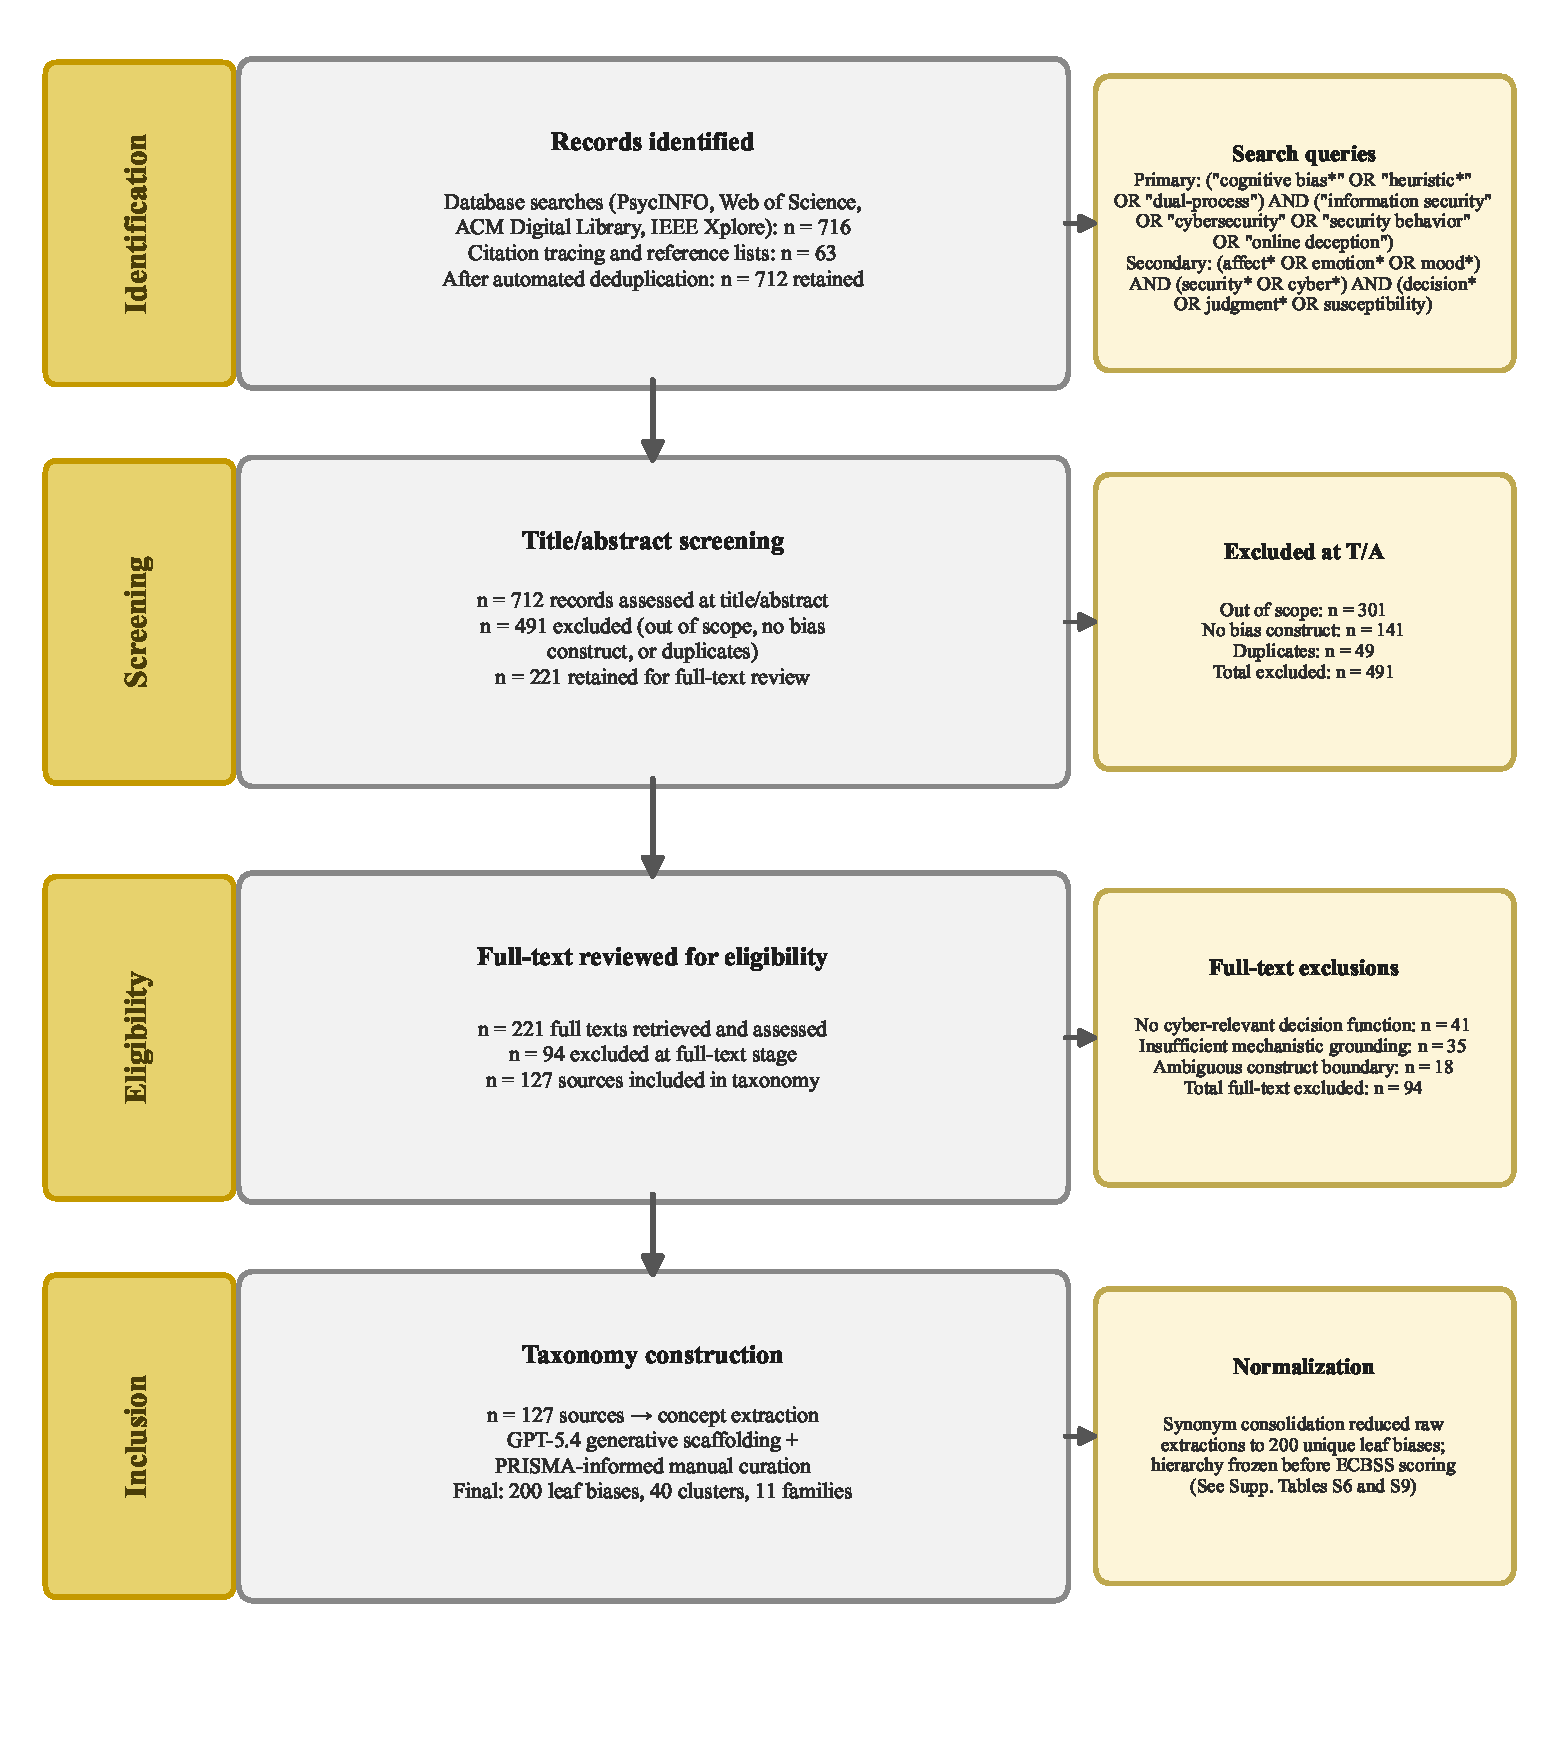
\includegraphics[width=0.95\textwidth]{../assets/figures/figSPRISMA_review_flow.pdf}
  \fignote{Top-down schematic of the preregistered review pipeline used to curate and freeze the taxonomy. The flow maps identification, screening, eligibility adjudication, and final inclusion logic used before taxonomy output freeze.}
\end{figure}

\begin{figure}[!htb]
  \raggedright
  \caption{Full emotion-by-family \ecbss{} clustermap with distributional summaries}
  \label{fig:s2}
  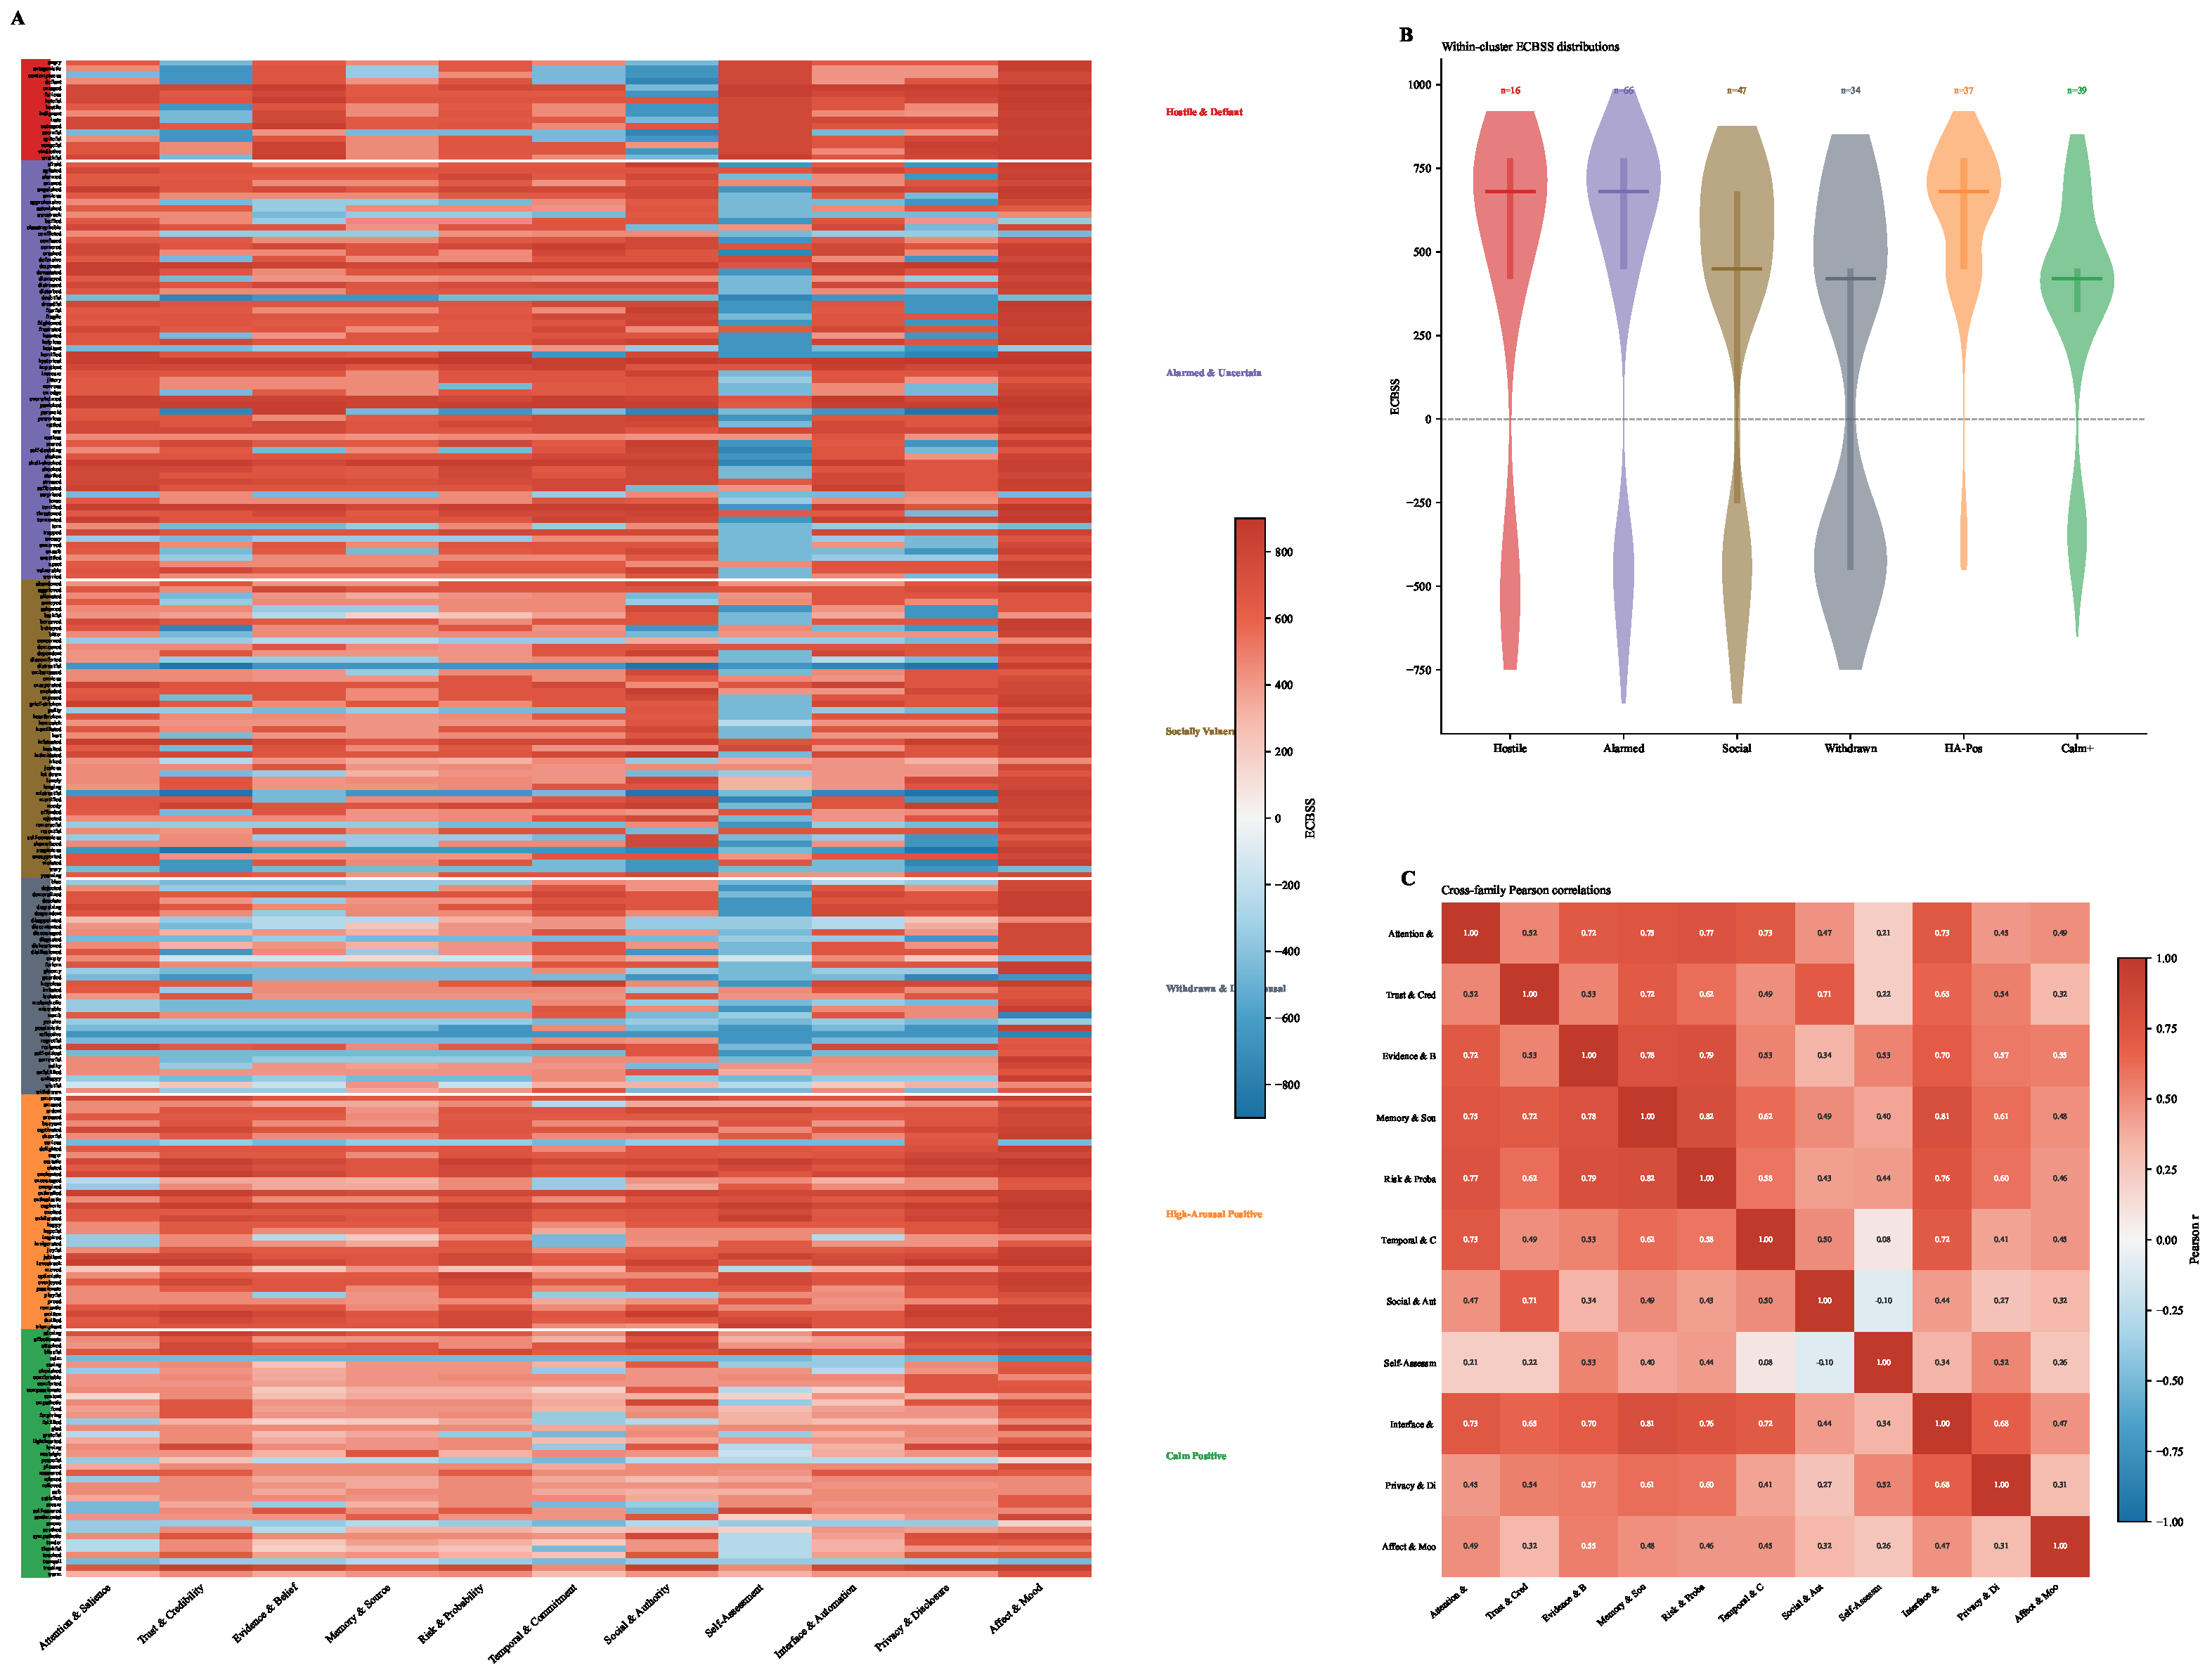
\includegraphics[width=\textwidth]{../assets/figures/figS1_full_ecbss_clustermap.pdf}
  \fignote{Panel A: Complete $239 \times 11$ \ecbss{} matrix with hierarchical clustering on both axes. Red cells indicate amplification; blue cells indicate attenuation. Left color bar shows cluster assignment; horizontal white lines mark cluster boundaries. Panel B: Within-cluster \ecbss{} distributions (violin + box) pooled across all 11 families, illustrating heterogeneity inside each cluster. Annotation shows $n$ = number of emotions per cluster.}
\end{figure}

\begin{figure}[p]
  \raggedright
  \caption{UMAP visualization colored by affective components}
  \label{fig:s3}
  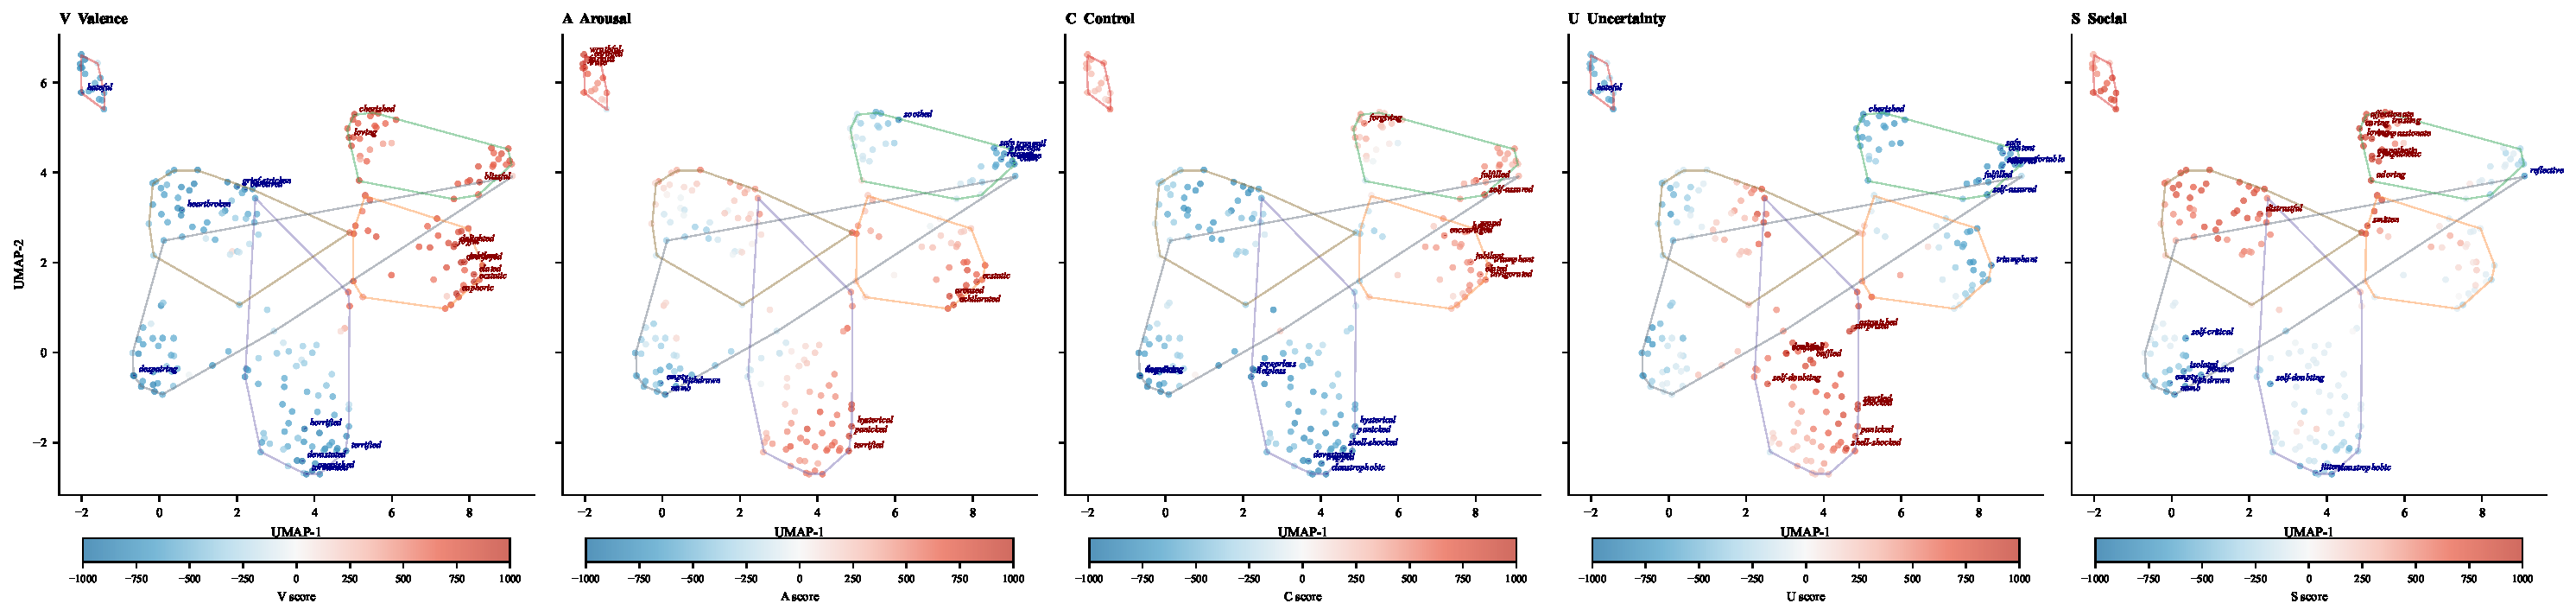
\includegraphics[width=\textwidth]{../assets/figures/figS2_umap_dimensional_scoring.pdf}
  \fignote{Five panels showing the same UMAP embedding colored by each \vacus{} component. Components here refer to the five theoretically motivated axes on which each emotion was rated: \textbf{V}alence (how positive/negative the feeling is), \textbf{A}rousal (how activating/energizing), \textbf{C}ontrol (how much the person feels able to cope), \textbf{U}ncertainty (how ambiguous the situation feels), and \textbf{S}ocial orientation (how prosocially vs.\ antisocially directed the state is). Each panel reveals a distinct gradient, confirming that the five components occupy non-redundant regions of the emotion manifold.}
\end{figure}

\begin{figure}[!t]
  \raggedright
  \caption{Principal component analysis of the affective-component emotion space}
  \label{fig:s4}
  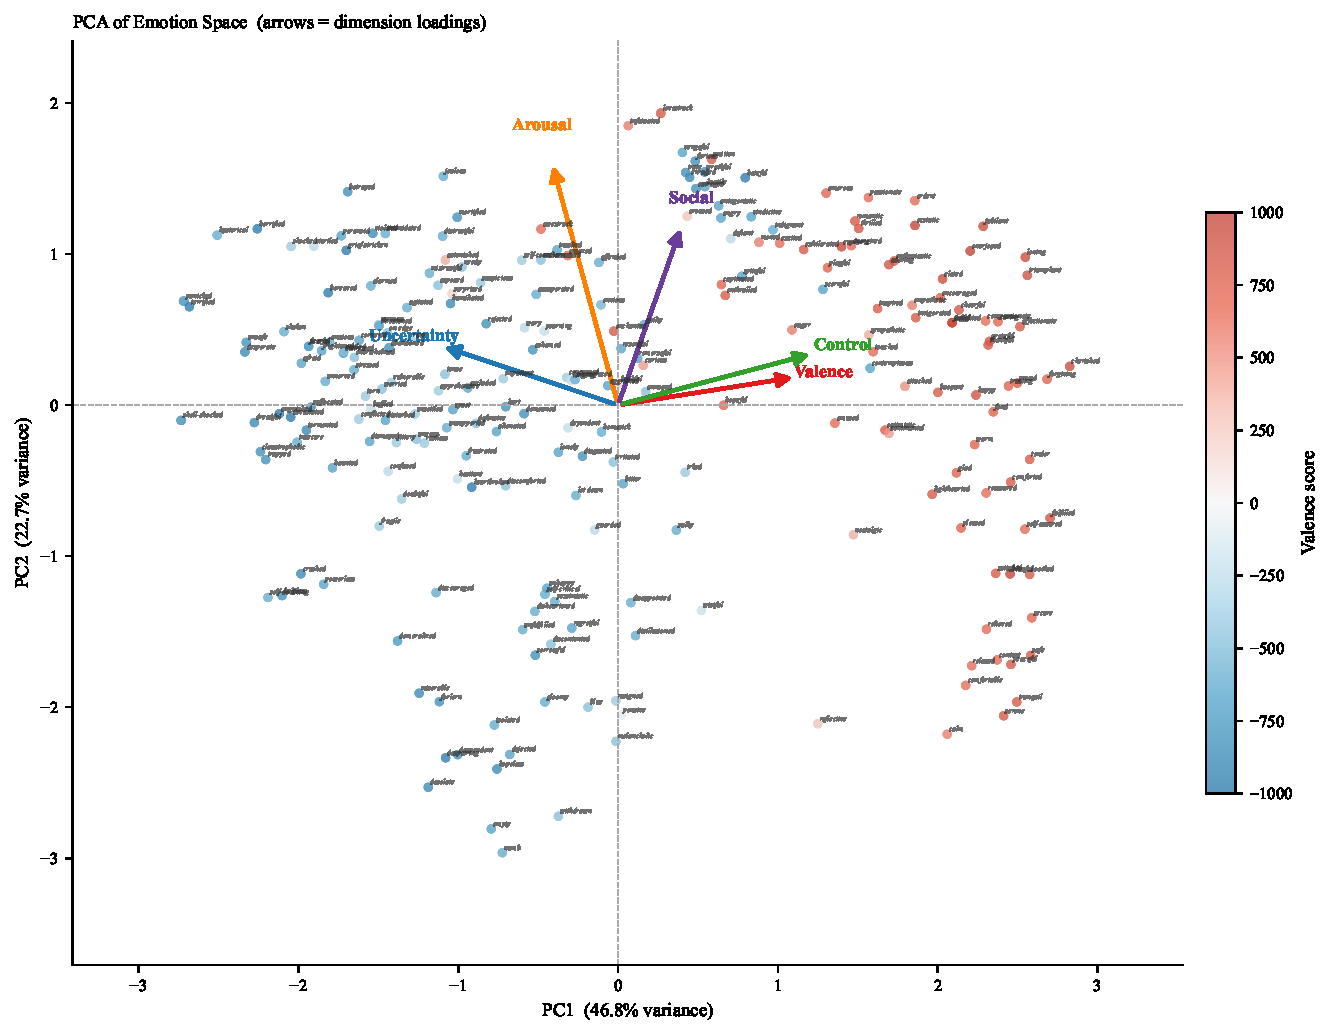
\includegraphics[width=\textwidth]{../assets/figures/figS3_pca_biplot.pdf}
  \fignote{PCA biplot of the standardized \vacus{} matrix. PC1 (46.8\% of variance) aligns primarily with the valence--control axis; PC2 (22.7\%) captures the arousal--uncertainty contrast; PC3 (17.7\%) adds additional social-orientation structure. Together the first three components explain 87.1\% of total variance. All 239 emotion states are annotated at reduced font size. Loading arrows show the directional contribution of each affective component to the principal components.}
\end{figure}

\begin{figure}[!t]
  \raggedright
  \caption{Cluster-solution diagnostics}
  \label{fig:s5}
  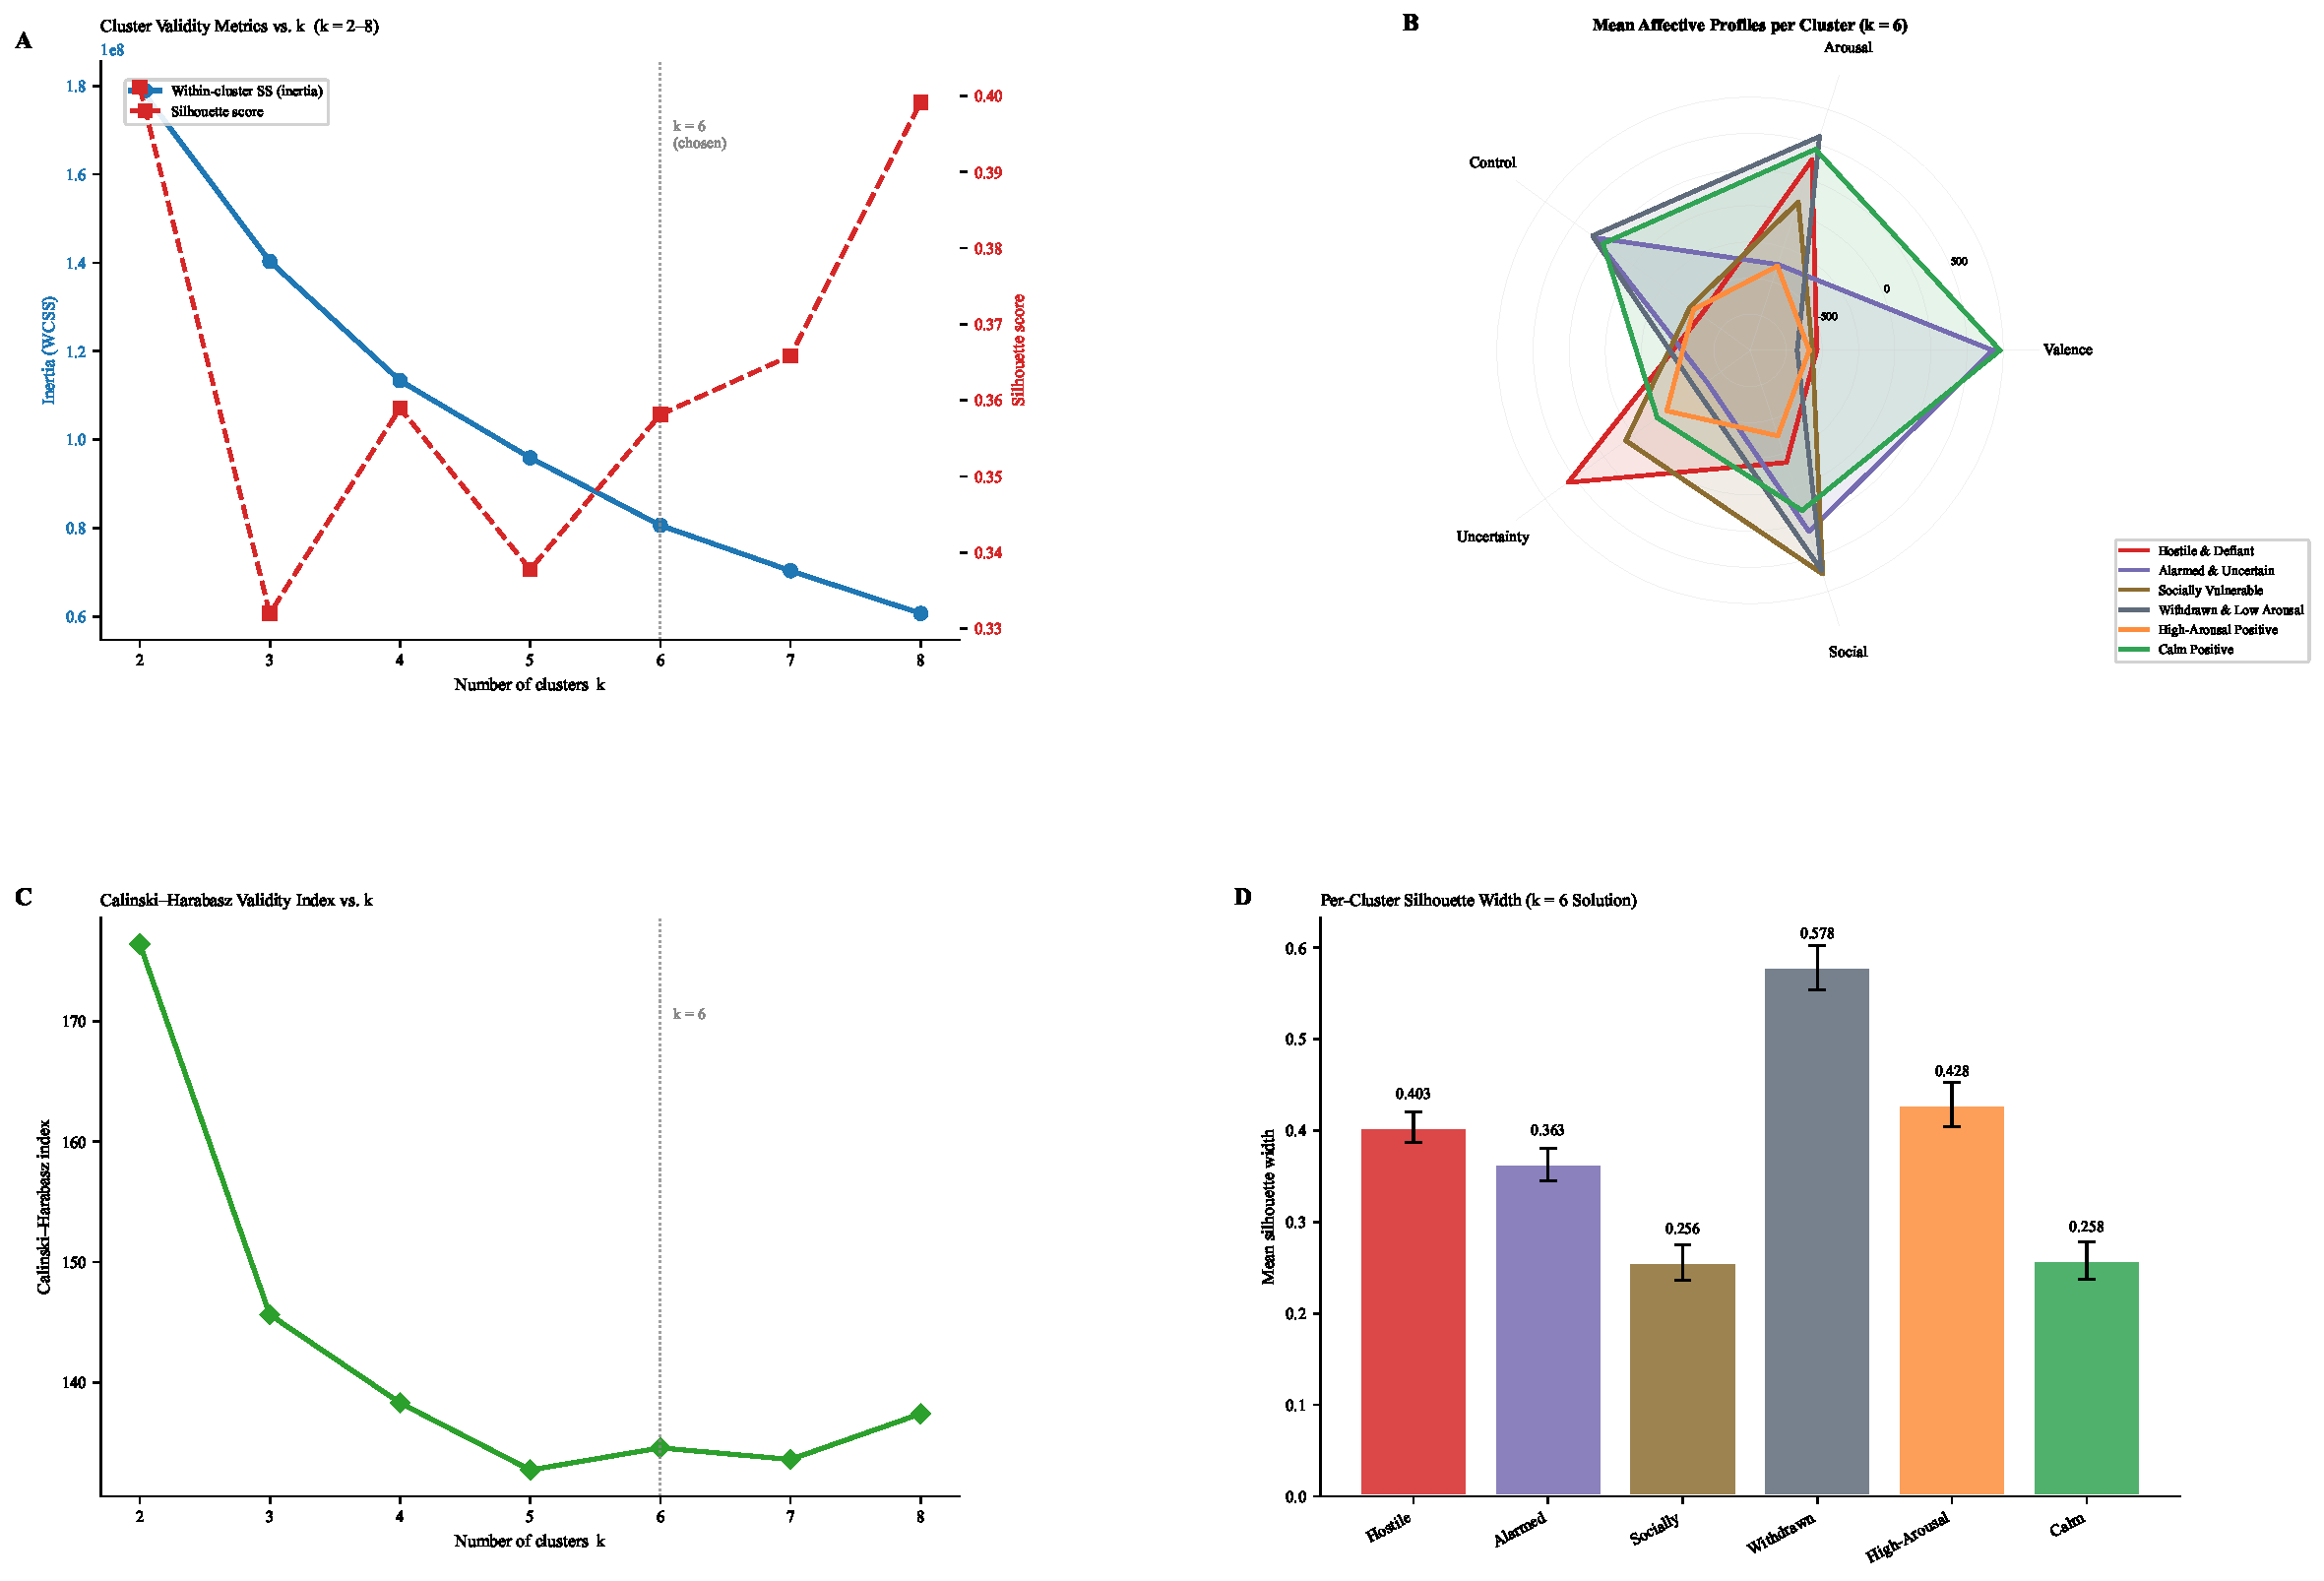
\includegraphics[width=\textwidth]{../assets/figures/figS4_cluster_validation.pdf}
  \fignote{Panel A: Elbow curve (inertia, left axis) and silhouette score (right axis) vs.\ $k = 2$--8; dotted line marks the chosen $k = 6$ solution. Panel B: Radar profiles of mean \vacus{} scores per cluster (normalized to $[-1, 1]$). Panel C: Calinski--Harabasz validity index vs.\ $k$; higher values indicate more compact, well-separated clusters. Panel D: Mean silhouette width $\pm$ SEM per cluster for the $k = 6$ solution; all positive values confirm within-cluster cohesion exceeds between-cluster separation. The preregistered $k = 6$ was retained for component-theoretic interpretability despite silhouette peaking at $k = 8$.}
\end{figure}

\clearpage
\begin{figure}[!t]
  \raggedright
  \caption{Cosine similarity structure of bias families}
  \label{fig:s6}
  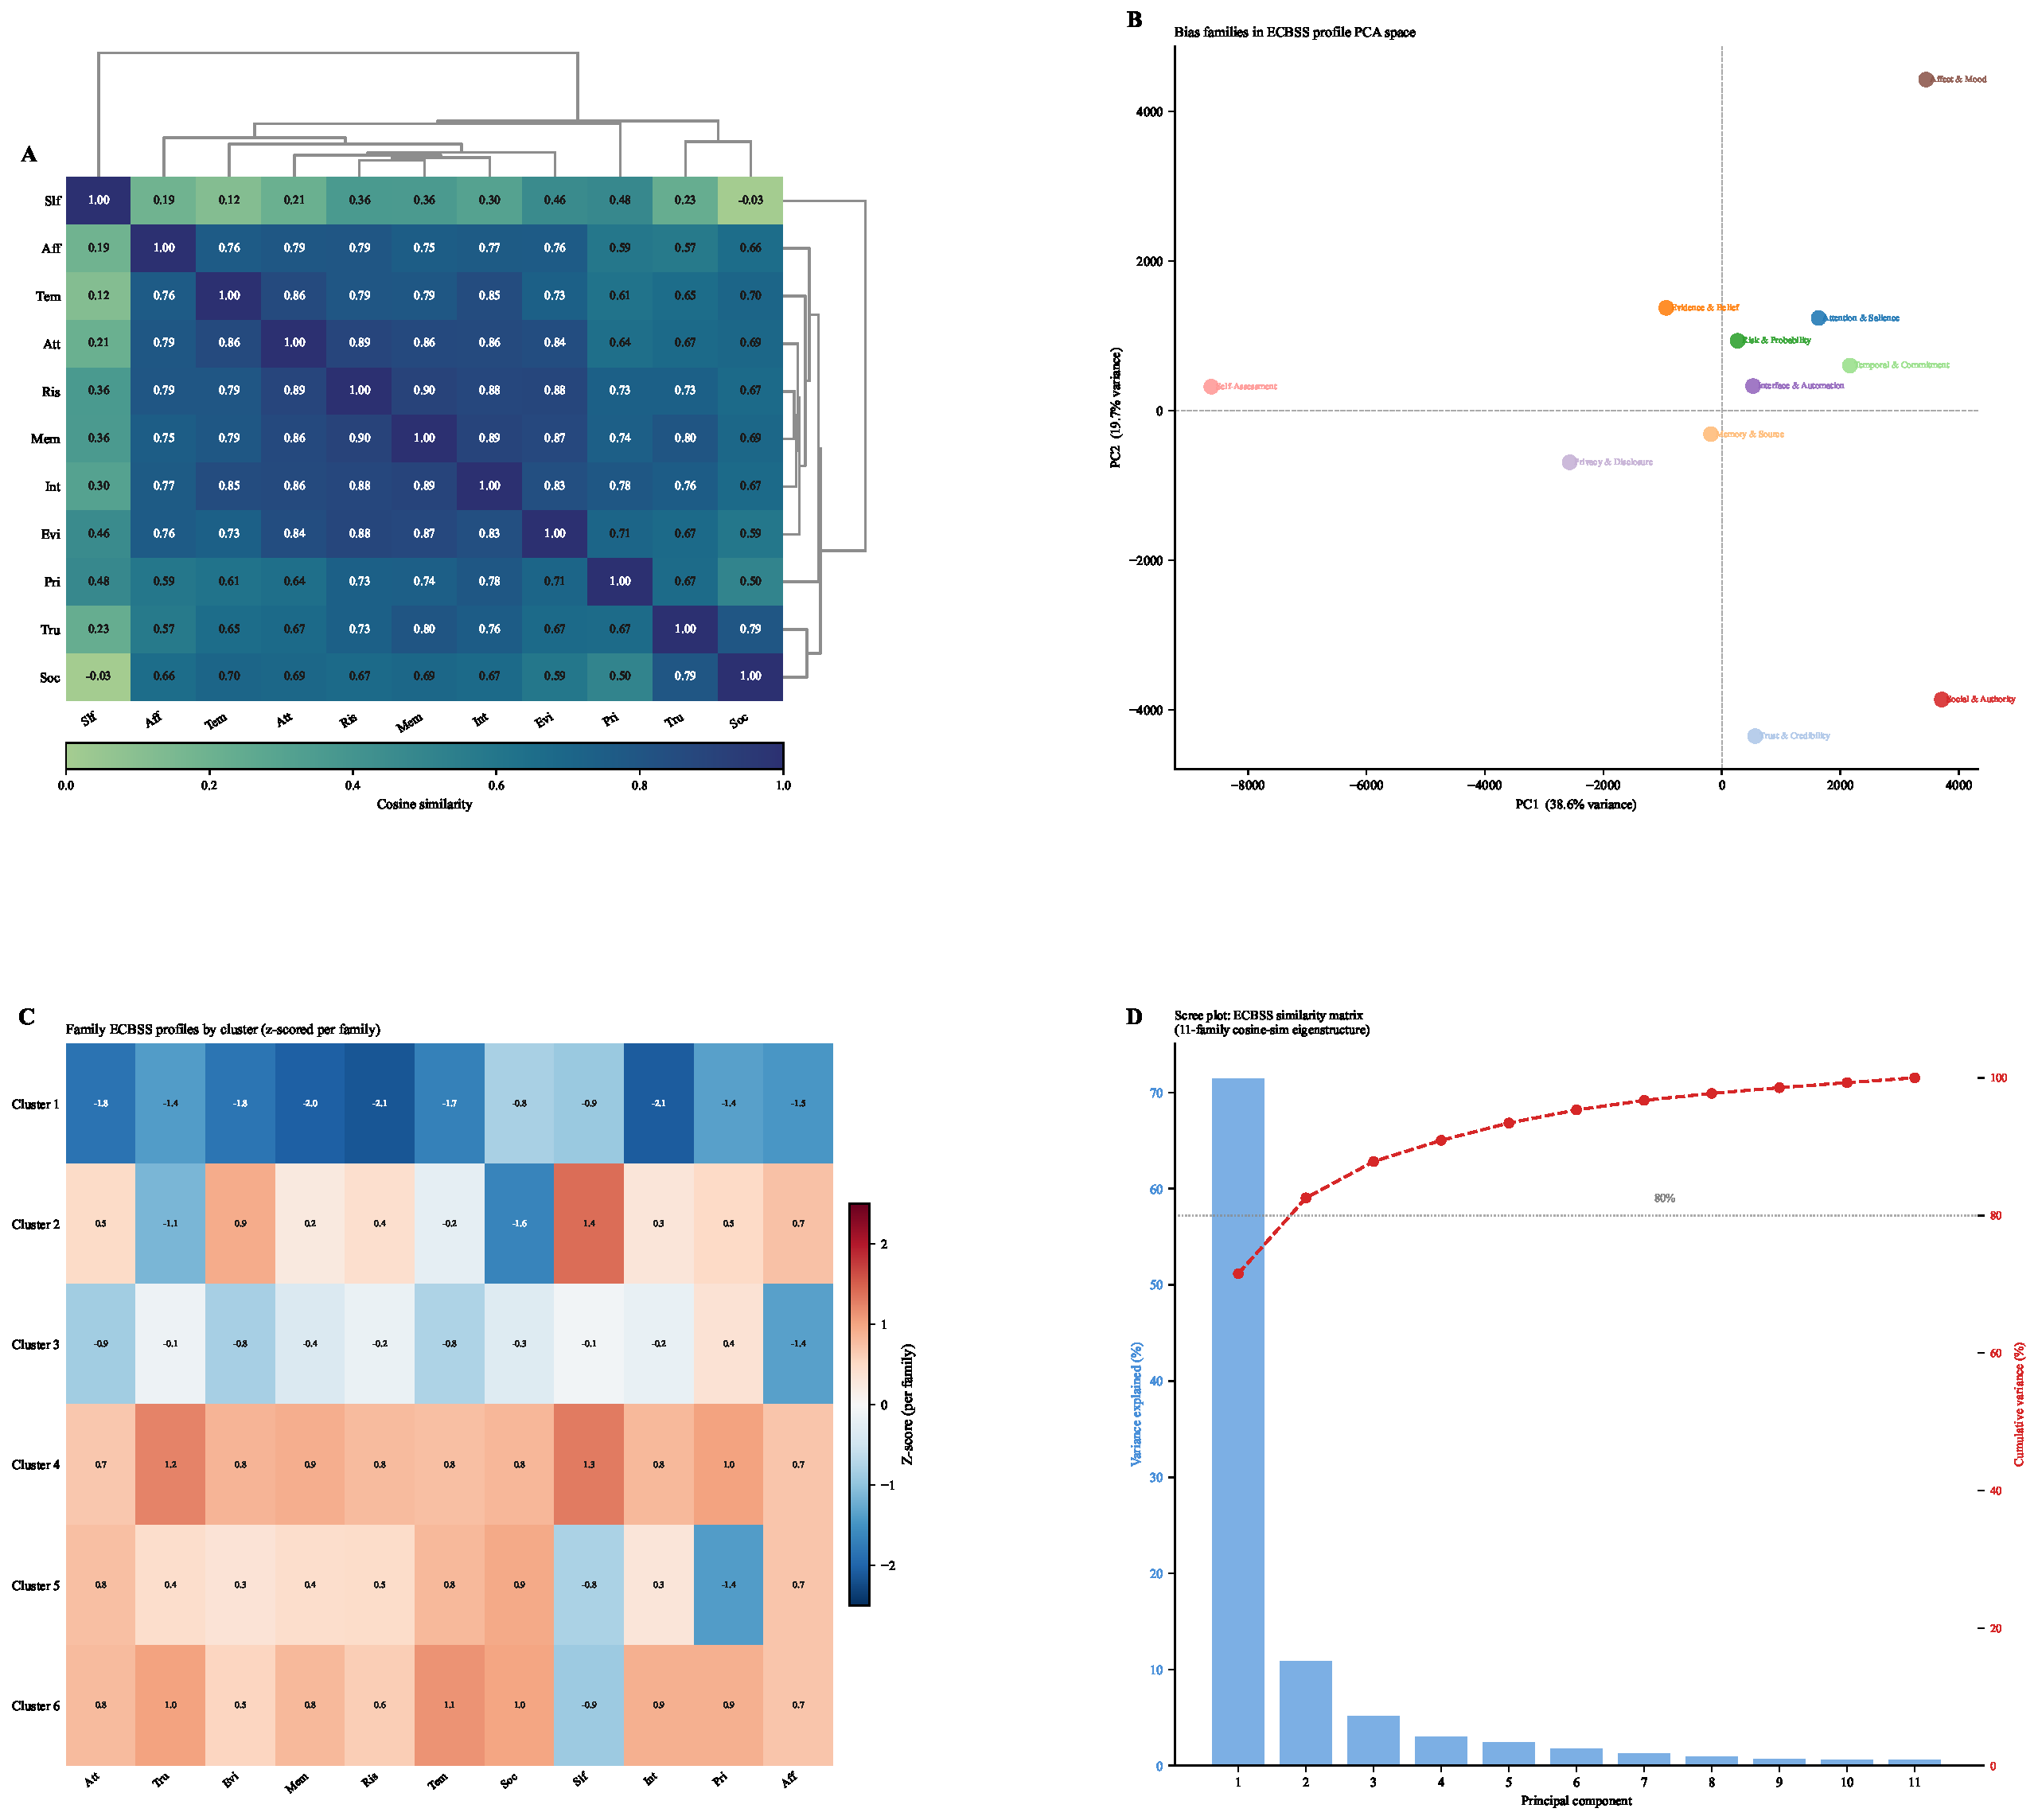
\includegraphics[width=\textwidth]{../assets/figures/figS5_bias_similarity.pdf}
  \fignote{Panel A: Pairwise cosine similarity of the 11 bias families computed from their 239-emotion \ecbss{} response profiles, with hierarchical clustering (average linkage, optimal leaf ordering) and aligned dendrograms. Panel B: PCA scatter of the 11 families in the space of their \ecbss{} profiles, showing the two dimensions of dominant between-family variation. Panel C: Normalized (z-scored per family) cluster-by-family \ecbss{} profile heatmap, revealing family-specific sensitivity patterns across emotion clusters independent of overall magnitude. Panel D: Scree plot of the eigenstructure of the $11 \times 11$ cosine-similarity matrix, showing how many principal components are needed to account for the bias-family similarity space.}
\end{figure}

\begin{figure}[!t]
  \raggedright
  \caption{Analytical-versus-direct \ecbss{} validation}
  \label{fig:s7}
  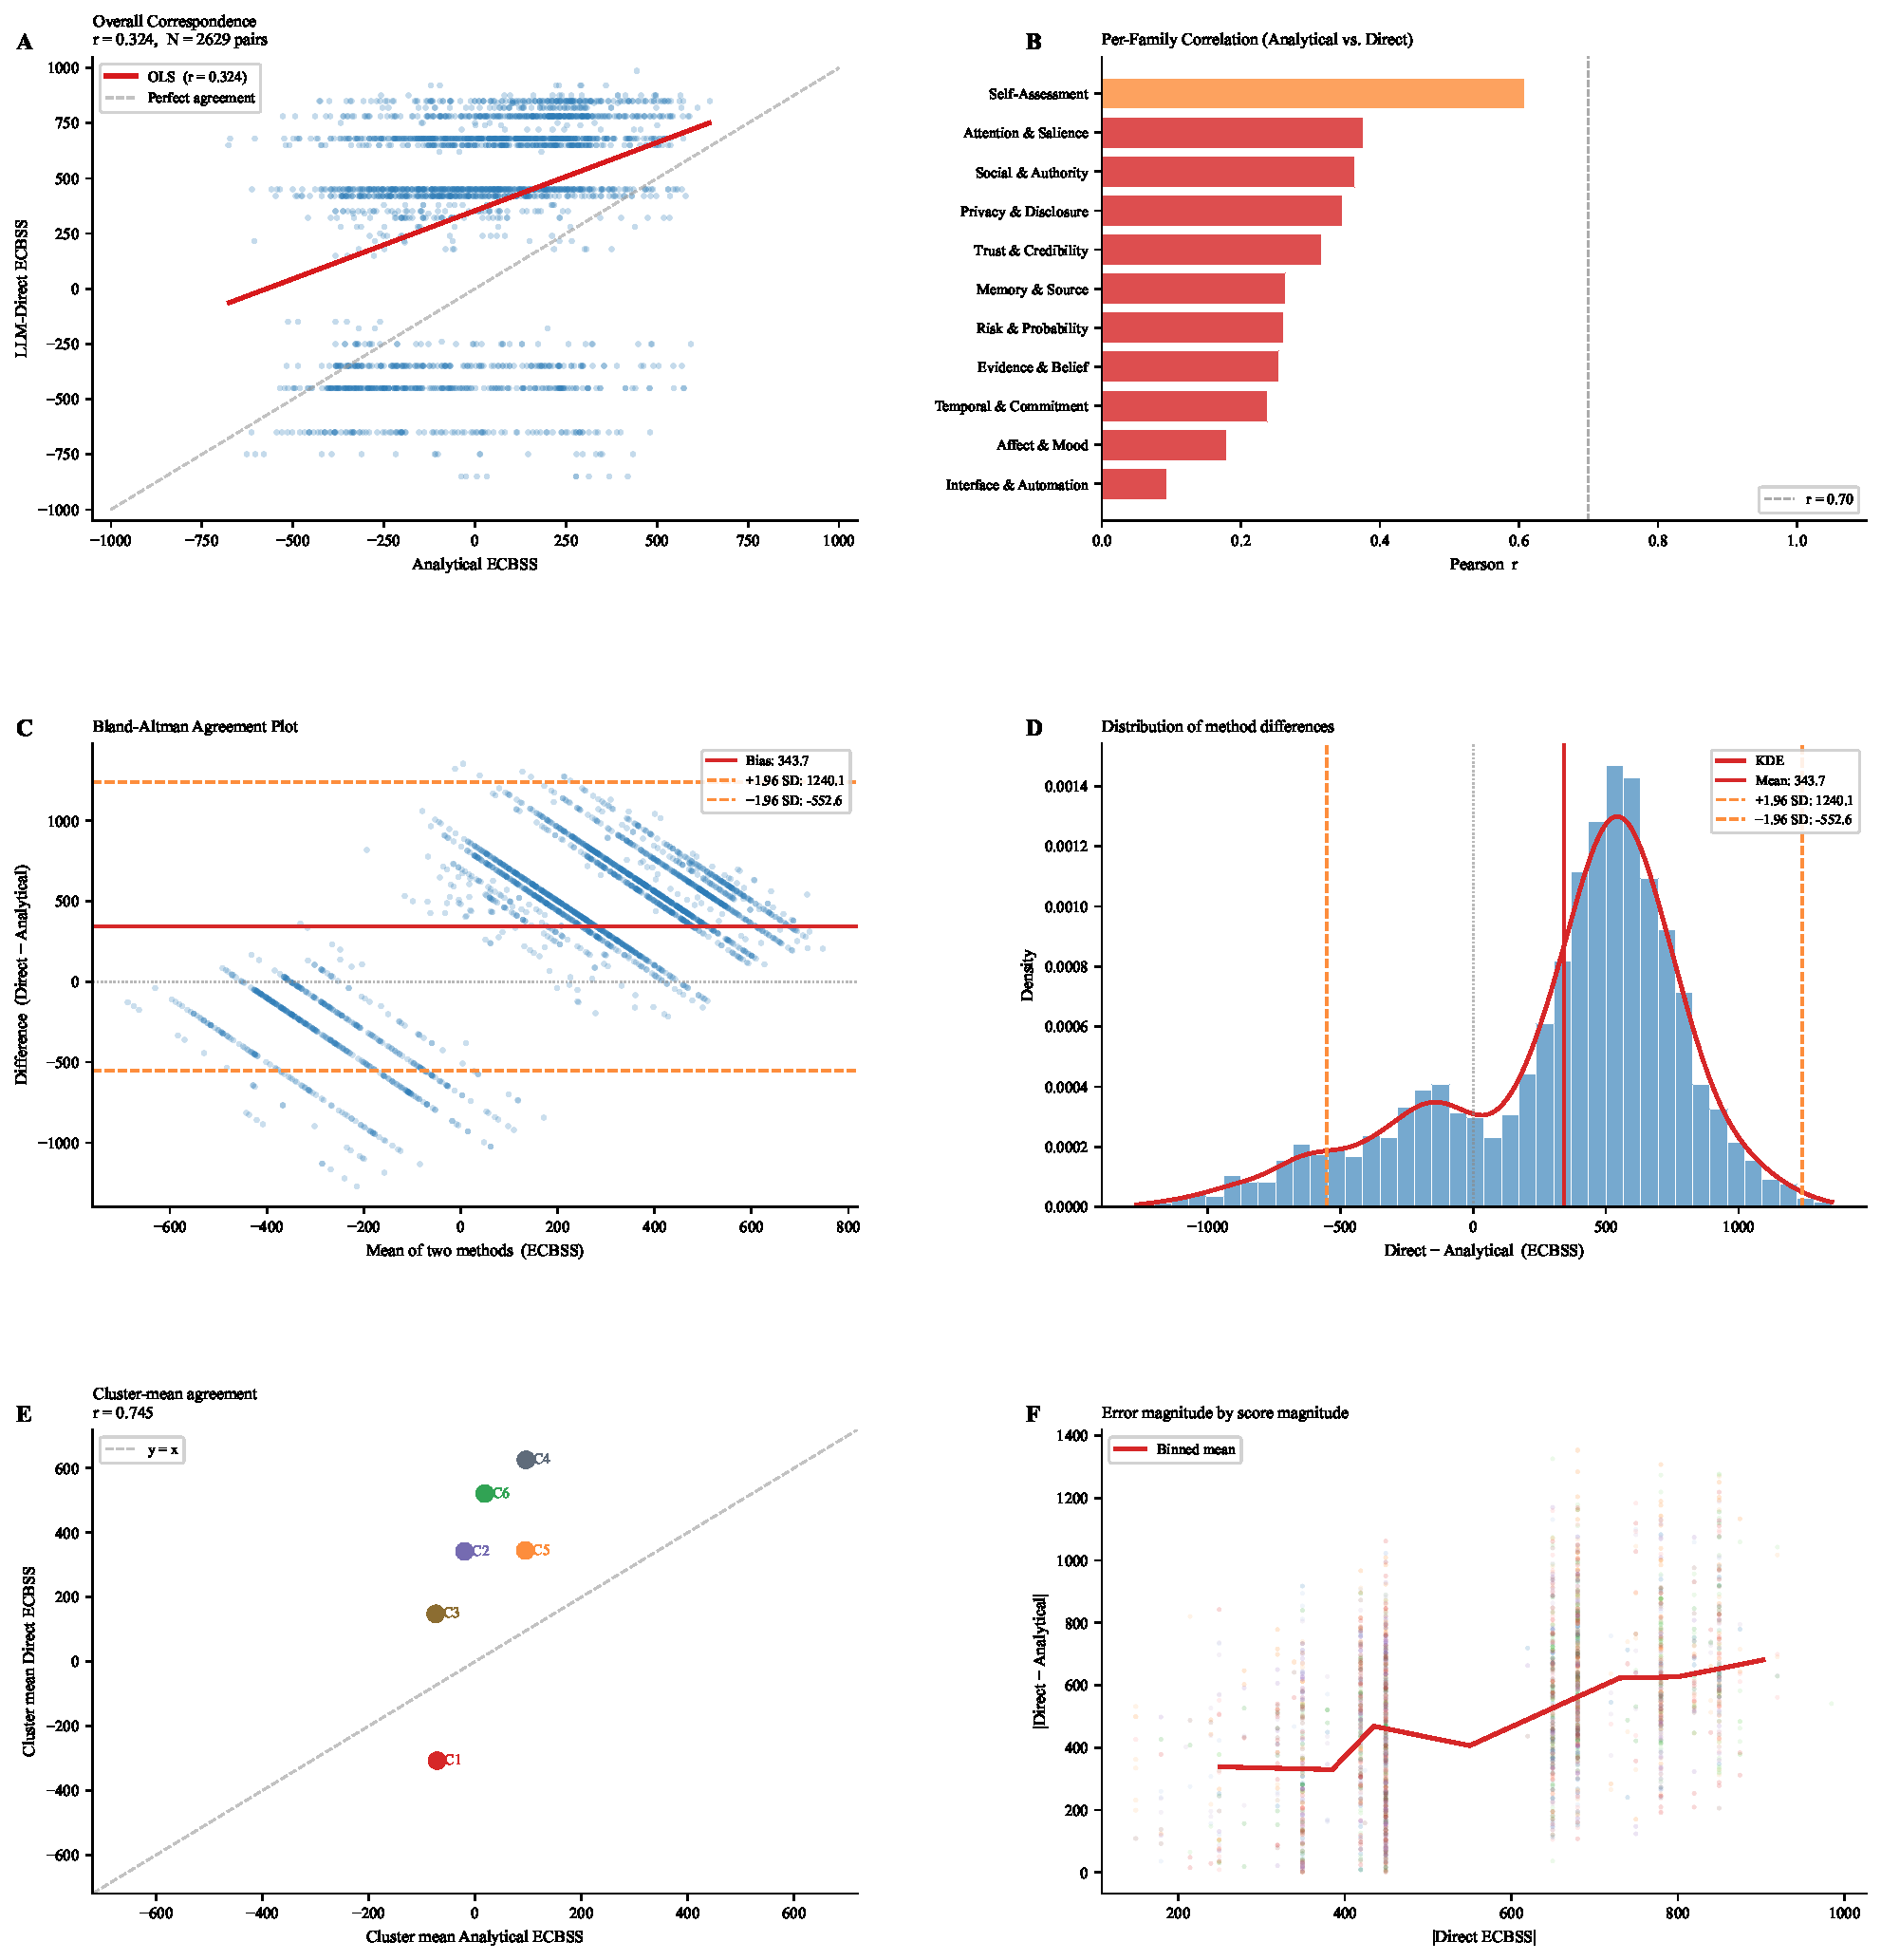
\includegraphics[width=\textwidth]{../assets/figures/figS6_validation_analysis.pdf}
  \fignote{Panel A: Overall scatter of all 2,629 direct vs.\ analytical scores with OLS fit. Panel B: Per-family Pearson $r$ between methods. Panel C: Bland--Altman plot (difference vs.\ mean) with limits of agreement ($\pm 1.96\,SD$). Panel D: Distribution of method differences (direct $-$ analytical) with KDE, mean, and limits of agreement. Panel E: Cluster-level mean agreement (direct vs.\ analytical means per cluster). Panel F: Absolute error ($|\mathrm{direct} - \mathrm{analytical}|$) as a function of score magnitude ($|\mathrm{direct}|$), showing how residual divergence scales with score extremity.}
\end{figure}

\begin{figure}[!t]
  \raggedright
  \caption{Composite-emotion non-additivity analysis}
  \label{fig:s8}
  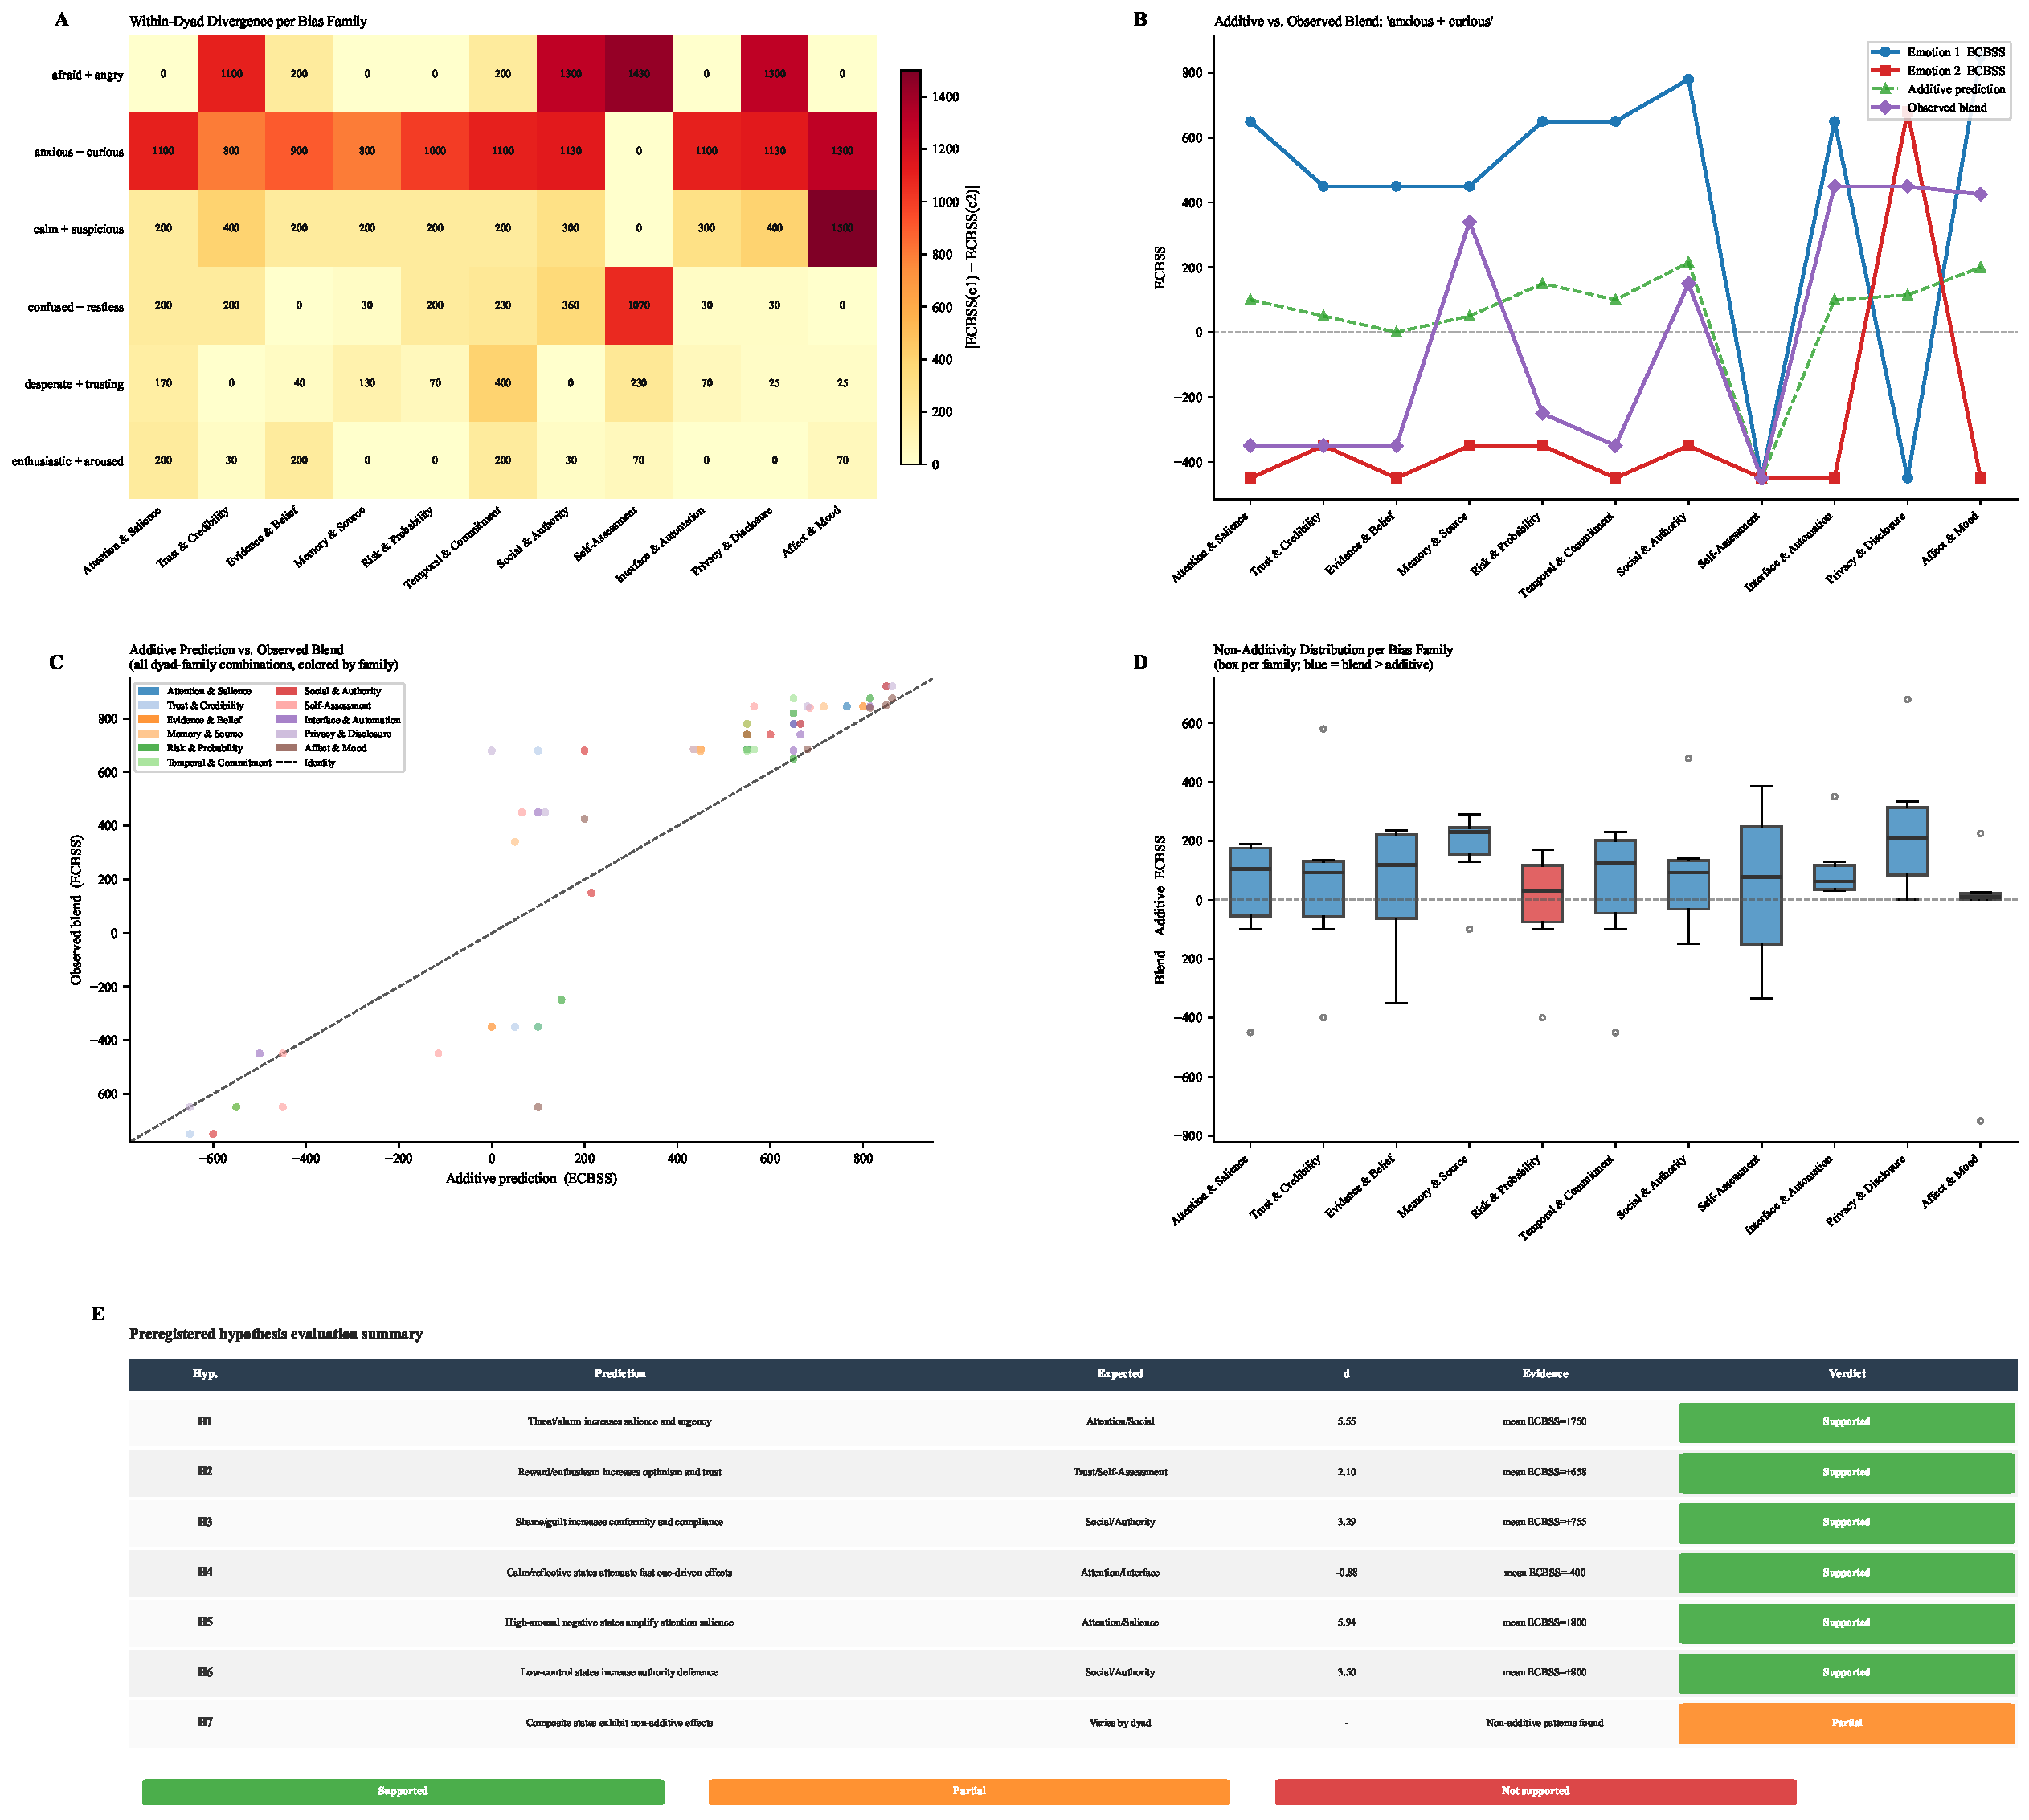
\includegraphics[width=\textwidth]{../assets/figures/figS8_composite_emotions.pdf}
  \fignote{Panel A: Absolute within-dyad divergence ($|\mathrm{ECBSS}(e_1) - \mathrm{ECBSS}(e_2)|$) per bias family for all emotion dyads. Panel B: ECBSS trajectories across families for the highest-divergence dyad, comparing component emotion scores and additive (mean) prediction. Panel C: Scatter plot of additive prediction versus observed blend \ecbss{} across all dyad-family combinations (colored by family); points above the identity line indicate super-additive blending. Panel D: Box plot of (blend $-$ additive) \ecbss{} per bias family showing the distribution of non-additivity across dyads. Panel E: Preregistered hypothesis verdict grid with effect-size summaries and directional support labels.}
\end{figure}

\clearpage
\begin{figure}[!t]
  \raggedright
  \caption{Bias-family sensitivity profiles, component coefficients, variance decomposition, and partial effect sizes}
  \label{fig:s9}
  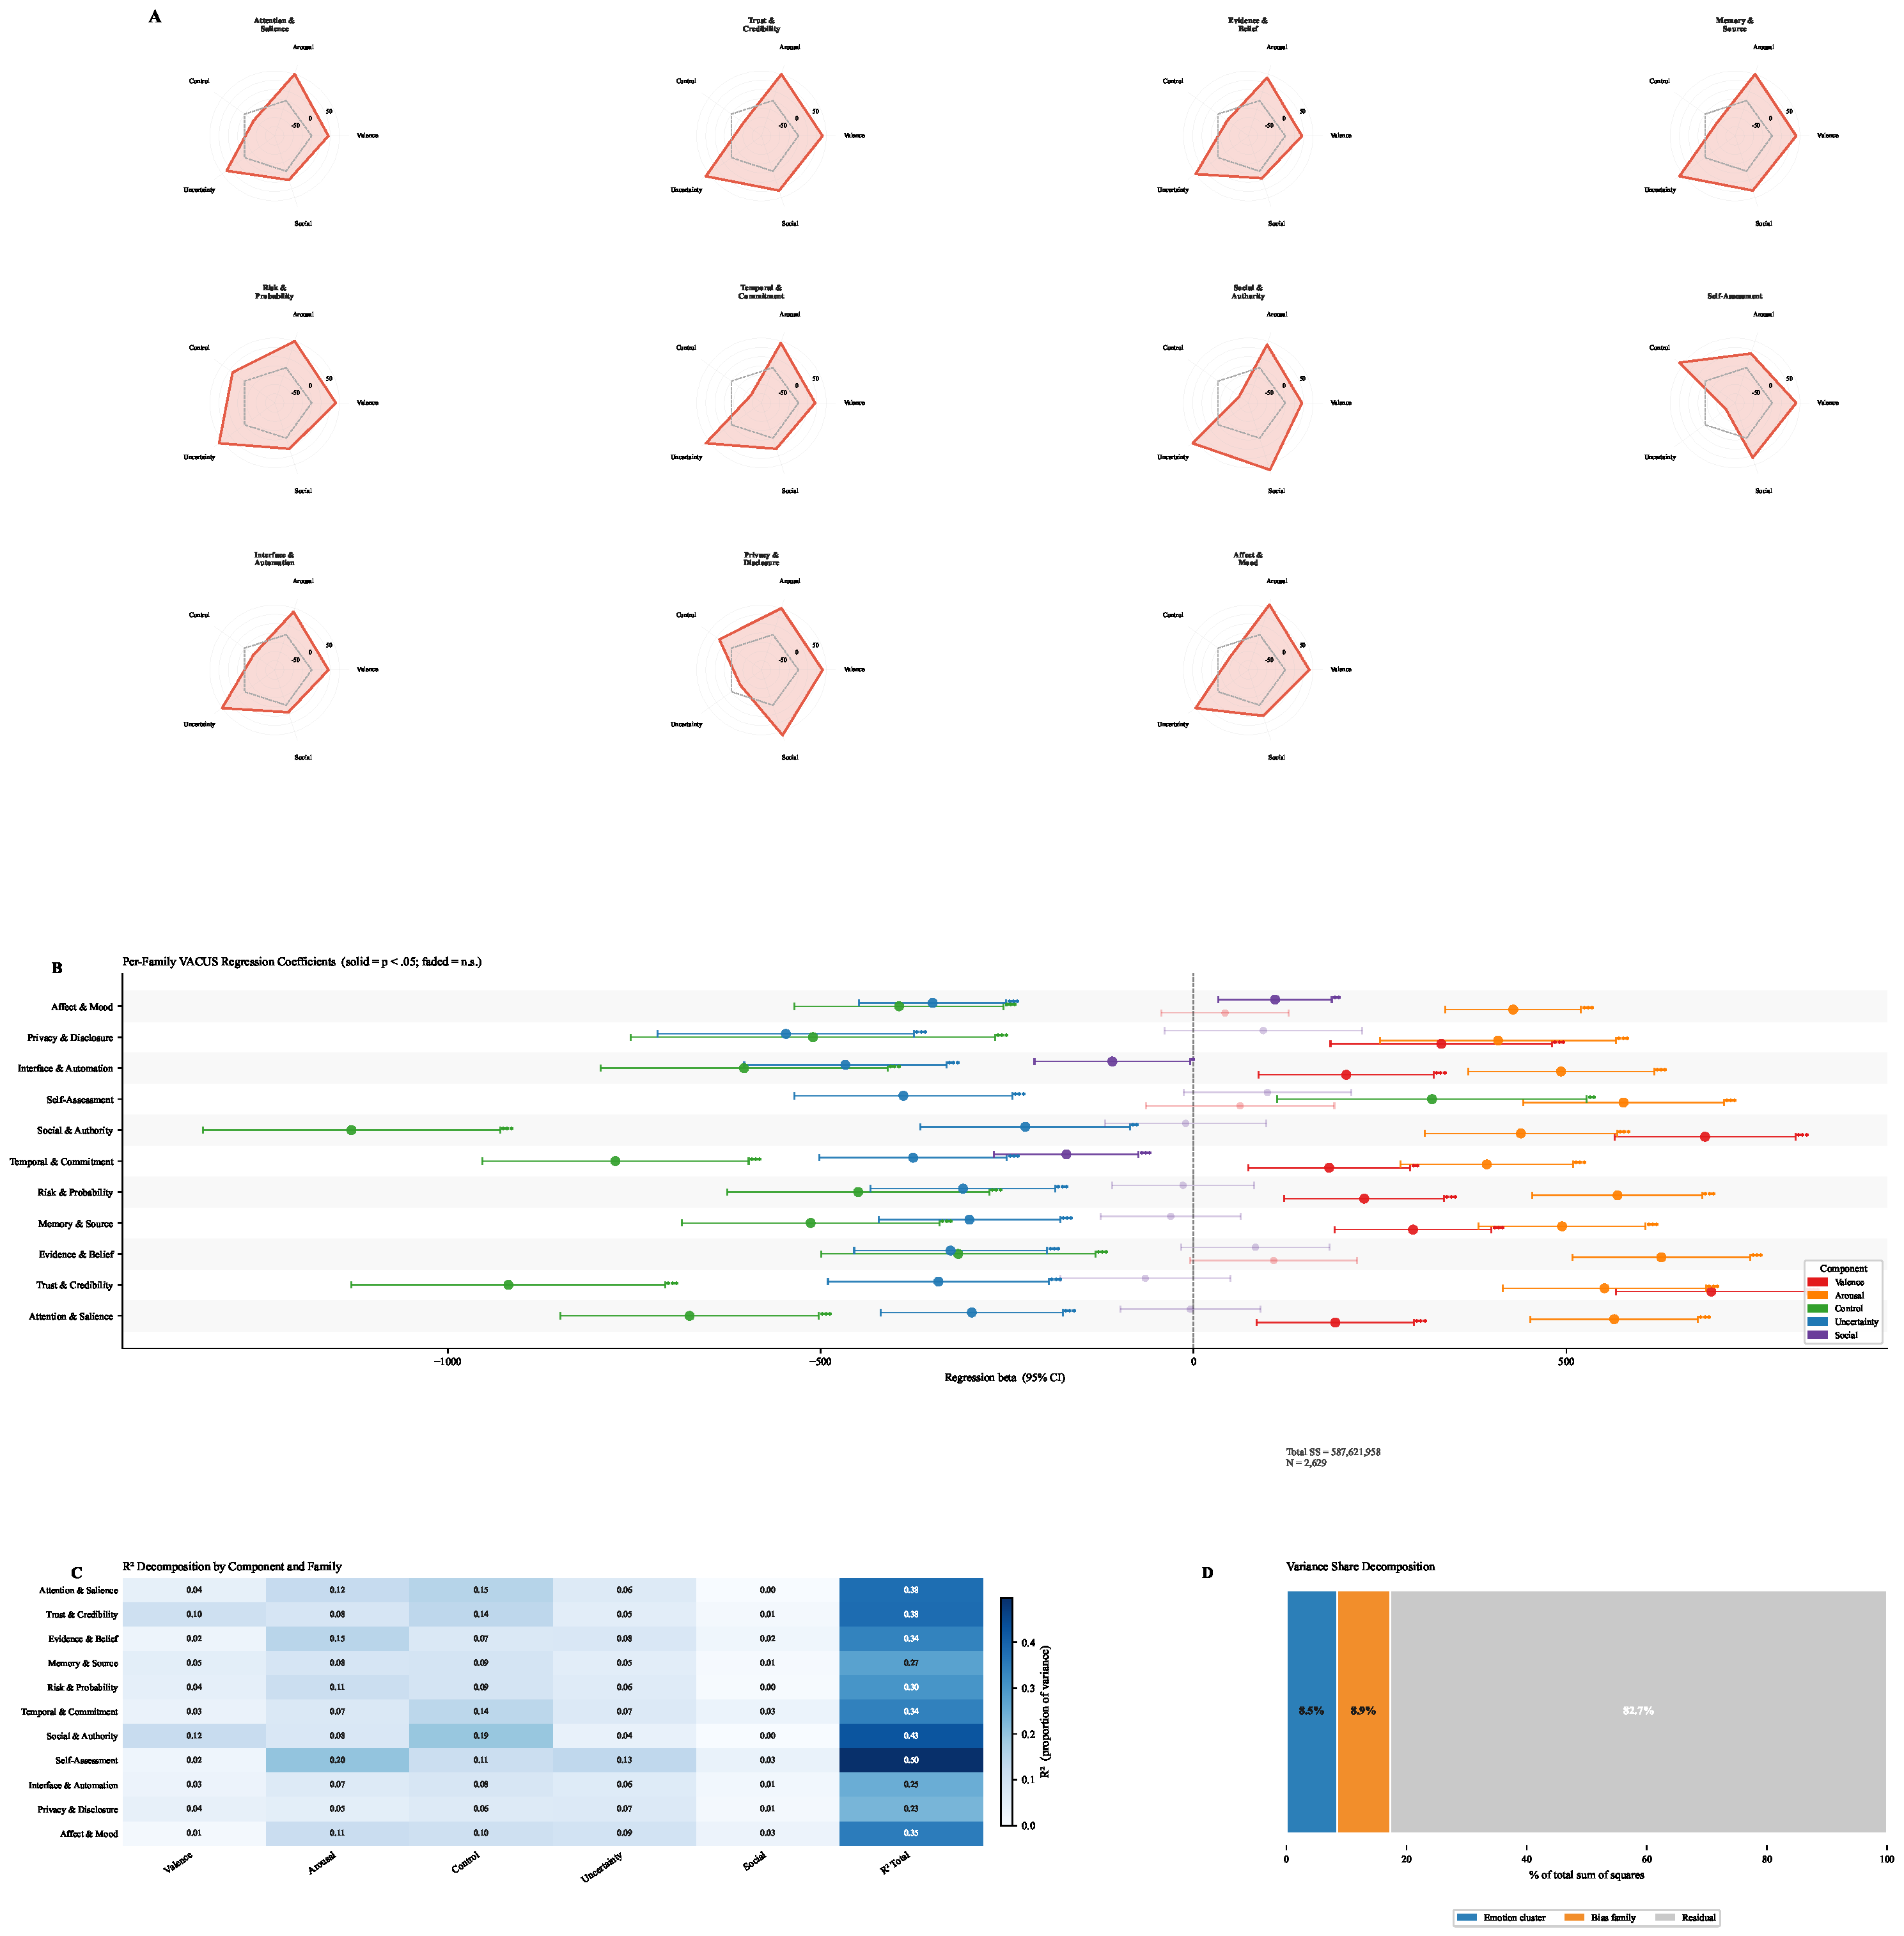
\includegraphics[width=\textwidth]{../assets/figures/figS9_combined.pdf}
  \fignote{Panel A: Radar profiles of family-level sensitivity weights across \vacus{} affective components (scale $-100$ to $+100$). Panel B: Per-family OLS regression coefficients ($\pm 95\%$ CI) for each affective component predicting \ecbss{}; filled circles indicate $p < .05$. Panel C: Variance explained ($R^2$) decomposition by component and family; columns show proportional $R^2$ per component plus total $R^2$. Panel D: Share of total \ecbss{} variance attributable to emotion cluster, bias family, and residual pair-specific effects.}
\end{figure}

\begin{figure}[!t]
  \raggedright
  \caption{Within-cluster distributional profiles}
  \label{fig:s11}
  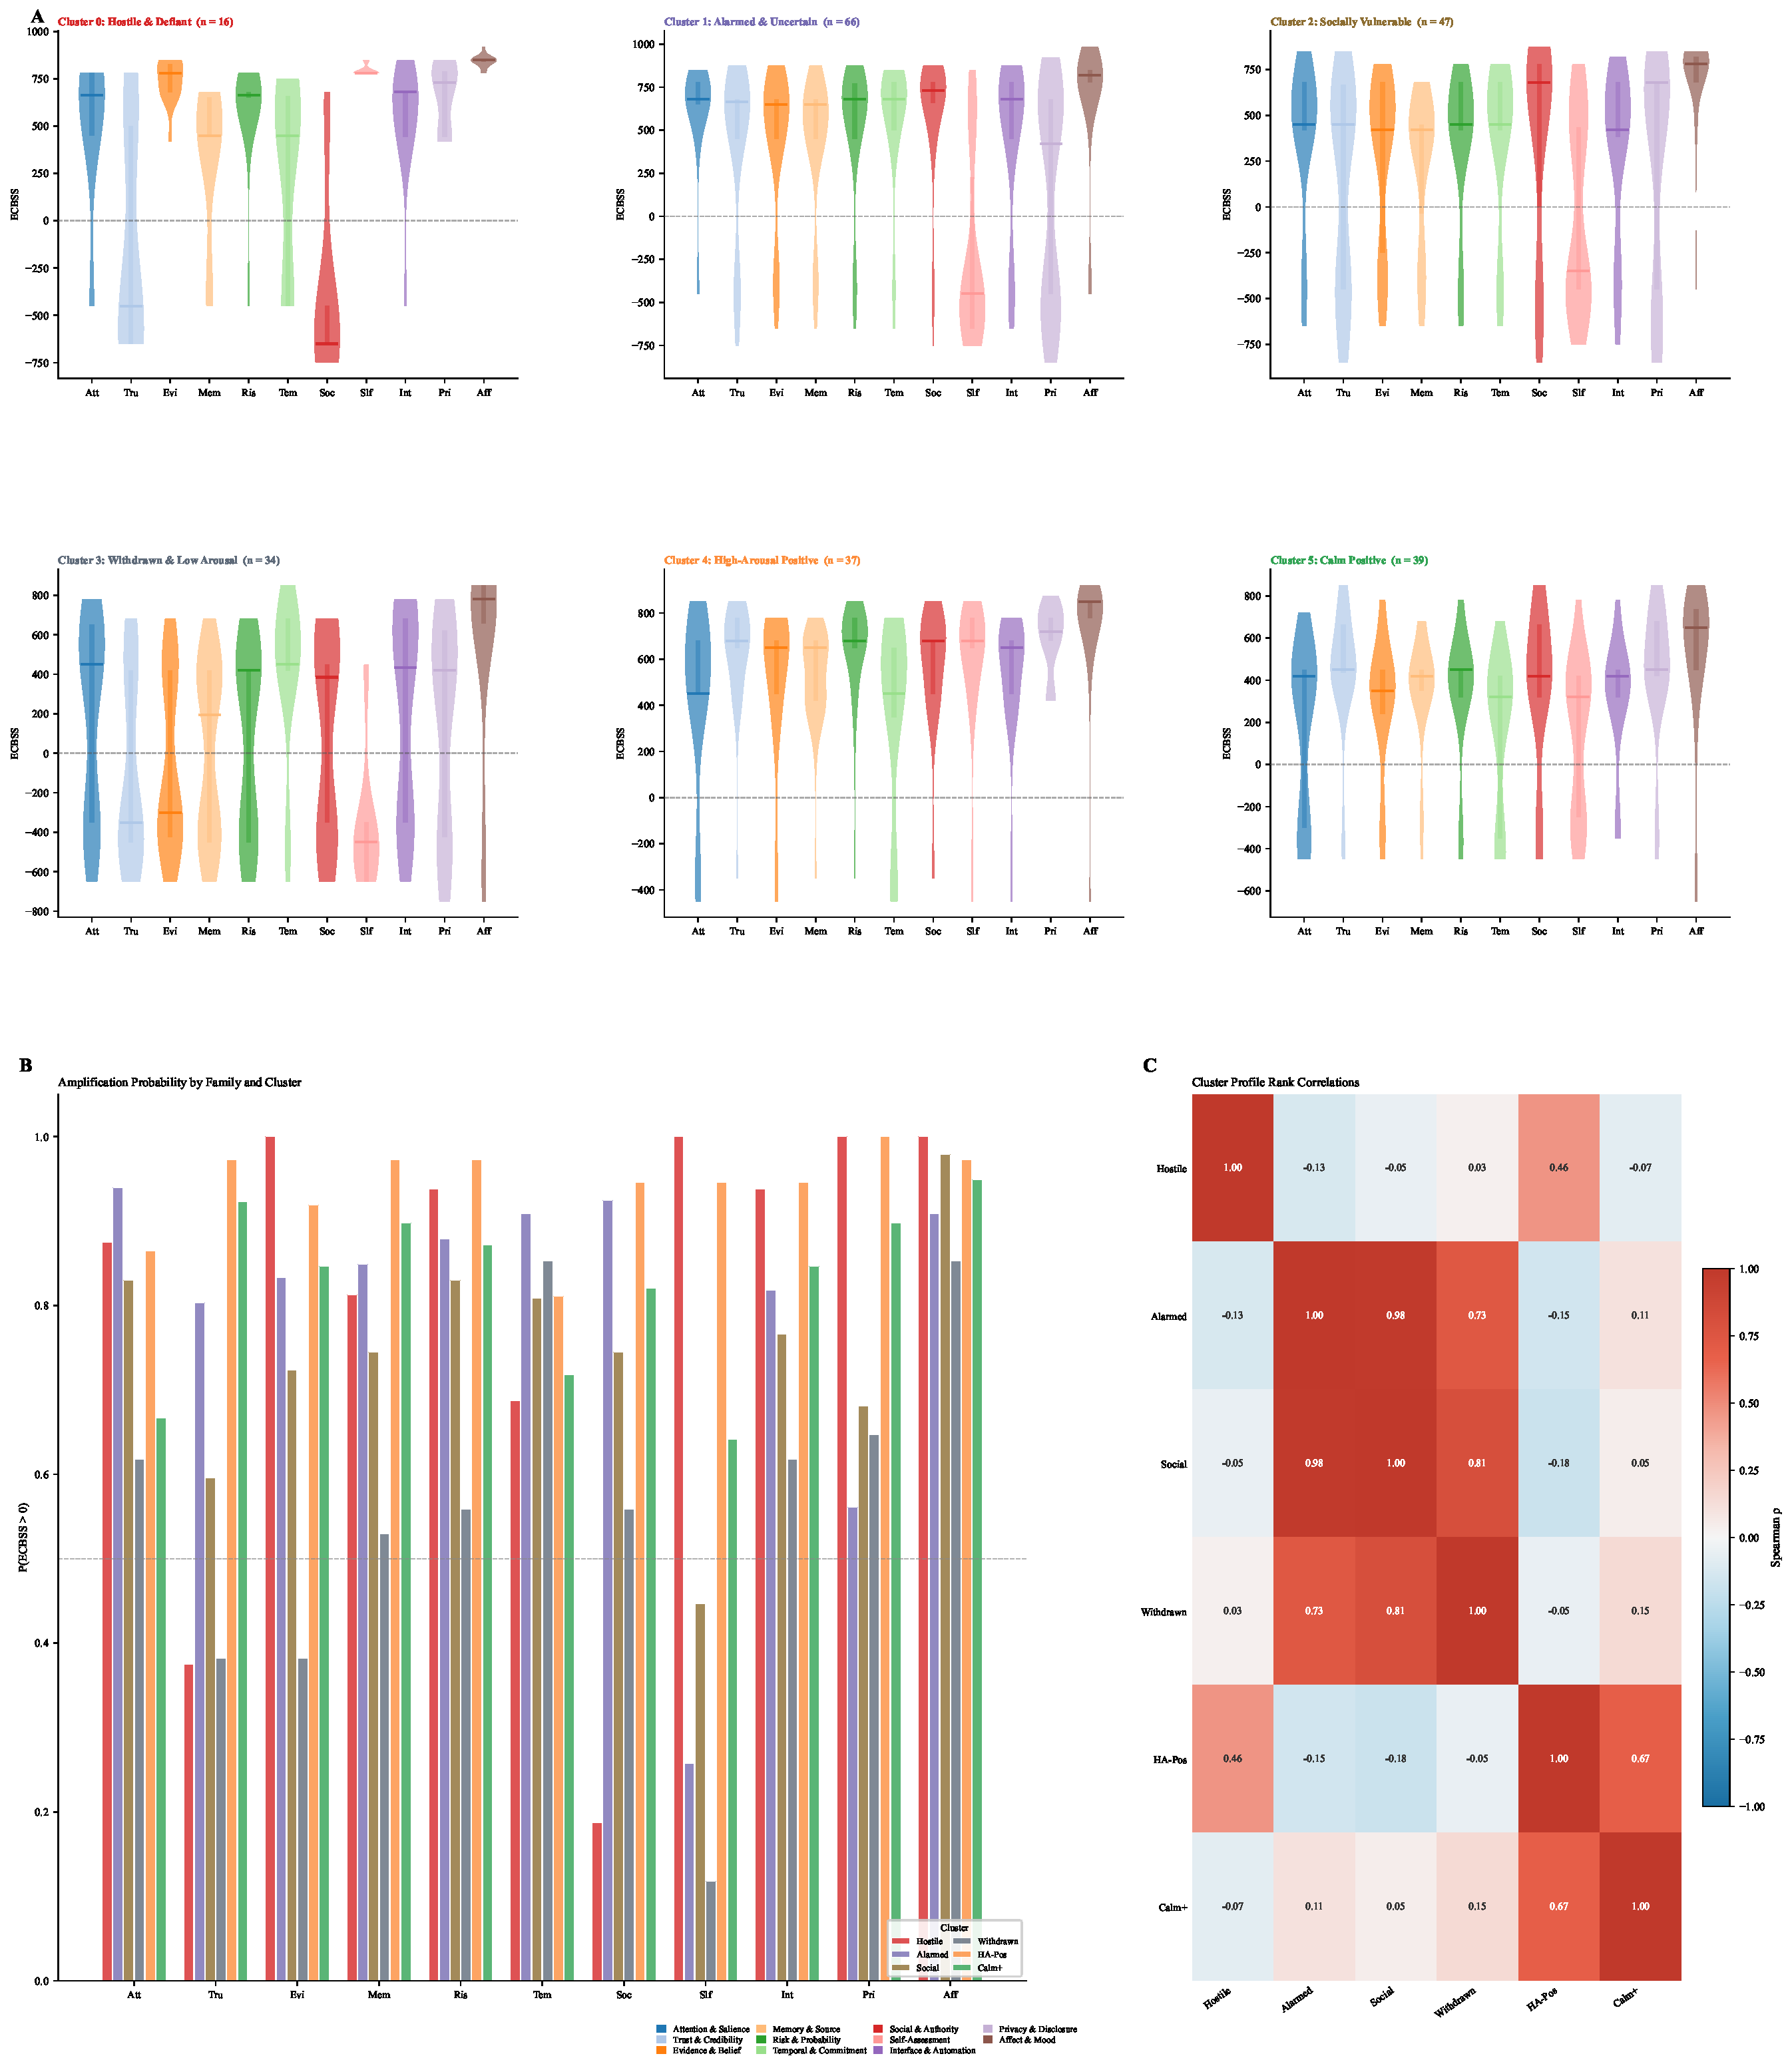
\includegraphics[width=\textwidth]{../assets/figures/figS10_emotion_profiles.pdf}
  \fignote{Panel A: Violin + box plots of \ecbss{} distributions by bias family for each of the six emotion clusters. Each violin is colored by family; horizontal bar = median; thick vertical bar = IQR. Panel B: Fraction of emotions within each cluster producing positive \ecbss{} (amplification probability) per family; dashed line at $P = 0.5$. Panel C: Spearman rank correlation matrix between pairs of clusters' family-level mean \ecbss{} profiles (6 $\times$ 6; diagonal = 1.0).}
\end{figure}

\clearpage
\subsection*{Supplementary Tables}

\begin{table}[H]
  \raggedright
  \small
  \caption{Taxonomy summary statistics}
  \label{tab:s1-taxonomy}
  \resizebox{\textwidth}{!}{\begin{tabular}{@{}p{0.22\textwidth}p{0.36\textwidth}rrr@{}}
\toprule
\footnotesize Bias family & \footnotesize Description & \footnotesize $n_{\mathrm{clusters}}$ & \footnotesize $n_{\mathrm{biases}}$ & \footnotesize Mean \ecbss{} \\
\midrule
\footnotesize Affect \& Mood & \footnotesize Biases in which current affective state systematically shapes evaluation, memory retrieval, and risk estimation. & \footnotesize 3 & \footnotesize 7 & \footnotesize $+682.00$ \\
\footnotesize Risk \& Probability & \footnotesize Systematic errors in estimating likelihoods, outcomes, and the comparative value of uncertain options. & \footnotesize 4 & \footnotesize 24 & \footnotesize $+424.54$ \\
\footnotesize Attention \& Salience & \footnotesize Systematic distortions in what information receives attentional priority during threat detection and signal evaluation. & \footnotesize 3 & \footnotesize 20 & \footnotesize $+414.12$ \\
\footnotesize Interface \& Automation & \footnotesize Biases arising from interaction with automated systems, interface defaults, and alert/warning responses. & \footnotesize 3 & \footnotesize 14 & \footnotesize $+395.71$ \\
\footnotesize Temporal \& Commitment & \footnotesize Biases relating to time-discounting, inertia, default acceptance, and escalating commitment to prior choices. & \footnotesize 4 & \footnotesize 17 & \footnotesize $+394.97$ \\
\footnotesize Social \& Authority & \footnotesize Distortions driven by social conformity, authority compliance, and identity-based information processing. & \footnotesize 5 & \footnotesize 24 & \footnotesize $+381.34$ \\
\footnotesize Evidence \& Belief & \footnotesize Biases in how evidence is sought, weighted, and integrated during hypothesis testing and belief revision. & \footnotesize 5 & \footnotesize 38 & \footnotesize $+355.60$ \\
\footnotesize Memory \& Source & \footnotesize Distortions arising from how past information is encoded, retrieved, and attributed to its original source. & \footnotesize 3 & \footnotesize 14 & \footnotesize $+336.82$ \\
\footnotesize Privacy \& Disclosure & \footnotesize Systematic over- or under-disclosure driven by contextual norms, social desirability, and self-presentation concerns. & \footnotesize 2 & \footnotesize 6 & \footnotesize $+328.45$ \\
\footnotesize Trust \& Credibility & \footnotesize Errors in source authentication, authority attribution, and credibility assessment of information and communicators. & \footnotesize 3 & \footnotesize 14 & \footnotesize $+296.73$ \\
\footnotesize Self-Assessment & \footnotesize Errors in self-evaluation, attribution of outcomes to internal vs.\ external causes, and metacognitive accuracy. & \footnotesize 5 & \footnotesize 22 & \footnotesize $+45.38$ \\
\midrule
\footnotesize \textit{Total/Mean} & & \footnotesize 40 & \footnotesize 200 & \footnotesize $+368.79$ \\
\bottomrule
\end{tabular}
}
  \tabnote{Counts and mean \ecbss{} values (averaged over all 239 emotions) for the 11 bias families. Sorted by mean \ecbss{} descending. Full inventory in Supplementary Table~\ref{tab:s6-taxonomy}.}
\end{table}

\begin{table}[htb]
  \raggedright
  \small
  \caption{Top amplifying and attenuating emotion-family pairs}
  \label{tab:s2-pairs}
  \renewcommand{\arraystretch}{0.94}
  \resizebox{\textwidth}{!}{\begin{tabularx}{\linewidth}{@{}>{\raggedright\arraybackslash}X>{\raggedright\arraybackslash}p{3.8cm}>{\centering\arraybackslash}p{1.6cm}>{\centering\arraybackslash}p{1.6cm}@{}}
\toprule
Emotion & Bias family & ECBSS & Cluster \\
\midrule
\multicolumn{4}{@{}l}{\textbf{Highest amplifying pairs}} \\[2pt]
Hysterical & Affect \& Mood & $+$985 & Alarmed \\
Enraged & Affect \& Mood & $+$920 & Hostile \\
Terrified & Affect \& Mood & $+$920 & Alarmed \\
Ecstatic & Affect \& Mood & $+$920 & HA-Pos \\
Hysterical & Privacy \& Disclosure & $+$920 & Alarmed \\
Raw & Affect \& Mood & $+$920 & Alarmed \\
Panicked & Affect \& Mood & $+$920 & Alarmed \\
Euphoric & Affect \& Mood & $+$920 & HA-Pos \\
\midrule
\multicolumn{4}{@{}l}{\textbf{Strongest attenuating pairs}} \\[2pt]
Mistrustful & Social \& Authority & $-850$ & Social \\
Distrustful & Trust \& Credibility & $-850$ & Social \\
Suspicious & Privacy \& Disclosure & $-850$ & Social \\
Distrustful & Privacy \& Disclosure & $-850$ & Social \\
Suspicious & Trust \& Credibility & $-850$ & Social \\
Distrustful & Social \& Authority & $-850$ & Social \\
Paranoid & Privacy \& Disclosure & $-850$ & Alarmed \\
Mistrustful & Privacy \& Disclosure & $-850$ & Social \\
\bottomrule
\end{tabularx}
}
  \tabnote{Eight highest-amplifying and eight strongest-attenuating emotion-family pairs from the direct \ecbss{} matrix, with cluster assignment.}
\end{table}

\begin{table}[htb]
  \raggedright
  \small
  \caption{Per-family regression coefficients and variance explained}
  \label{tab:s3-regression}
  \resizebox{\textwidth}{!}{\begin{tabularx}{\linewidth}{Xrrrrrr}
\toprule
Bias family & $\beta_{V}$ & $\beta_{A}$ & $\beta_{C}$ & $\beta_{U}$ & $\beta_{S}$ & $R^2$ \\
\midrule
Attention \& Salience & $190.1^{***}$ & $564.2^{***}$ & $-675.7^{***}$ & $-297.3^{***}$ & $-4.2$ & 0.378 \\
Trust \& Credibility & $694.6^{***}$ & $551.2^{***}$ & $-918.7^{***}$ & $-342.0^{***}$ & $-64.7$ & 0.381 \\
Evidence \& Belief & $107.6$ & $627.3^{***}$ & $-315.6^{***}$ & $-325.6^{***}$ & $83.1$ & 0.338 \\
Memory \& Source & $294.5^{***}$ & $494.3^{***}$ & $-513.3^{***}$ & $-300.6^{***}$ & $-30.5$ & 0.274 \\
Risk \& Probability & $229.0^{***}$ & $568.6^{***}$ & $-449.6^{***}$ & $-309.0^{***}$ & $-14.1$ & 0.303 \\
Temporal \& Commitment & $182.0^{**}$ & $393.3^{***}$ & $-775.2^{***}$ & $-376.0^{***}$ & $-170.5^{***}$ & 0.341 \\
Social \& Authority & $686.1^{***}$ & $439.0^{***}$ & $-1129.2^{***}$ & $-225.5^{**}$ & $-10.5$ & 0.426 \\
Self-Assessment & $62.6$ & $576.8^{***}$ & $320.0^{**}$ & $-389.0^{***}$ & $99.2$ & 0.497 \\
Interface \& Automation & $204.9^{***}$ & $493.0^{***}$ & $-602.8^{***}$ & $-466.9^{***}$ & $-108.9^{*}$ & 0.249 \\
Privacy \& Disclosure & $332.3^{***}$ & $408.5^{***}$ & $-510.3^{***}$ & $-546.7^{***}$ & $93.7$ & 0.232 \\
Affect \& Mood & $42.3$ & $428.8^{***}$ & $-394.8^{***}$ & $-349.8^{***}$ & $109.5^{**}$ & 0.350 \\
\bottomrule
\end{tabularx}
}
  \tabnote{Per-family OLS regression of \ecbss{} on \vacus{} dimensions ($N = 239$ per family). ${}^{*}p < .05$, ${}^{**}p < .01$, ${}^{***}p < .001$.}
\end{table}

\begin{table}[htb]
  \raggedright
  \small
  \caption{Cluster-level mean \ecbss{} matrix (all 11 families)}
  \label{tab:s4-cluster}
  \resizebox{\textwidth}{!}{{\renewcommand{\tabcolsep}{7pt}
\begin{tabular}{lrrrrrrrrrrrr}
\toprule
Cluster & F1 & F2 & F3 & F4 & F5 & F6 & F7 & F8 & F9 & F10 & F11 & \textit{Mean} \\
\midrule
Hostile   & +515 & $-$128 & +741 & +356 & +590 & +256 & $-$379 & +793 & +553 & +662 & +843 & \textit{+437} \\
Alarmed   & +628 & +429 & +460 & +446 & +533 & +579 & +624 & $-$241 & +472 & +129 & +699 & \textit{+433} \\
Social    & +392 & +129 & +285 & +240 & +354 & +372 & +361 & $-$33 & +315 & +225 & +732 & \textit{+307} \\
Withdrawn & +191 & $-$82 & $-$51 & +16 & +79 & +412 & +99 & $-$381 & +225 & +160 & +559 & \textit{+112} \\
HA-Pos    & +469 & +639 & +534 & +523 & +649 & +392 & +574 & +613 & +547 & +697 & +764 & \textit{+582} \\
Calm+     & +179 & +457 & +295 & +364 & +347 & +155 & +367 & +151 & +308 & +448 & +558 & \textit{+330} \\
\bottomrule
\end{tabular}
}
}
  \tabnote{Mean \ecbss{} for each of the six emotion clusters across all 11 bias families, with row means. Family codes: F1\,=\,Attention \& Salience; F2\,=\,Trust \& Credibility; F3\,=\,Evidence \& Belief; F4\,=\,Memory \& Source; F5\,=\,Risk \& Probability; F6\,=\,Temporal \& Commitment; F7\,=\,Social \& Authority; F8\,=\,Self-Assessment; F9\,=\,Interface \& Automation; F10\,=\,Privacy \& Disclosure; F11\,=\,Affect \& Mood. \ecbss{} range: $-1000$ to $+1000$. These numeric values underlie Figure~\ref{fig:heatmap}.}
\end{table}

\begin{table}[htb]
  \raggedright
  \small
  \caption{Emotion-cluster profiles and representative states}
  \label{tab:s5-clusters}
  \resizebox{\textwidth}{!}{\begin{tabularx}{\textwidth}{lcrrrrr>{\raggedright\arraybackslash}X}
\toprule
Cluster & $n$ & V & A & C & U & S & Representative emotions \\
\midrule
Hostile \& Defiant & 16 & -674 & 554 & 346 & -540 & 601 & indignant, angry, vindictive, hostile, outraged, antagonistic \\
Alarmed \& Uncertain & 66 & -507 & 397 & -586 & 561 & -171 & unnerved, rattled, afraid, on edge, disturbed, stressed \\
Socially Vulnerable & 47 & -545 & 101 & -491 & 78 & 634 & embarrassed, hurt, self-conscious, envious, needy, rejected \\
Withdrawn \& Low Arousal & 34 & -556 & -385 & -462 & -274 & -366 & gloomy, unfulfilled, pessimistic, blue, disheartened, melancholic \\
High-Arousal Positive & 37 & 737 & 456 & 302 & -273 & 145 & enthusiastic, inspired, eager, joyful, delighted, passionate \\
Calm Positive & 39 & 690 & -371 & 325 & -638 & 343 & reassured, warm, glad, sentimental, comforted, soothed \\
\bottomrule
\end{tabularx}
}
  \tabnote{Mean \vacus{} scores per cluster (scale $-1000$ to $+1000$) and centroid-nearest representative emotions. \textbf{V} = valence; \textbf{A} = arousal; \textbf{C} = control/coping; \textbf{U} = uncertainty; \textbf{S} = social orientation.}
\end{table}

\clearpage
\begingroup
\small
\raggedright
\begin{longtable}{p{0.20\textwidth}@{\hspace{20pt}}p{0.59\textwidth}r}
\caption{Taxonomy clusters grouped by bias family with mechanistic descriptions}\label{tab:s6-taxonomy}\\
\toprule
Taxonomy cluster & Mechanistic description & $n_{\mathrm{biases}}$ \\
\midrule
\endfirsthead
\multicolumn{3}{@{}l}{\textbf{Table \thetable\ (continued)}}\\
\multicolumn{3}{@{}p{\textwidth}@{}}{Taxonomy clusters grouped by bias family with mechanistic descriptions}\\
\toprule
Taxonomy cluster & Mechanistic description & $n_{\mathrm{biases}}$ \\
\midrule
\endhead
\midrule
\multicolumn{3}{r}{\textit{Continued on next page}}\\
\endfoot
\bottomrule
\endlastfoot
\addlinespace[2pt]\multicolumn{3}{@{}l}{\textbf{Attention \& Salience} ($n_{\mathrm{clusters}}=3$, $n_{\mathrm{biases}}=20$)} \\
Attentional Selection Under Load & Selective allocation of cognitive resources under high cognitive load distorts threat detection. & 8 \\
Salience Prominence And Vividness & Vivid, novel, or prominent stimuli capture attention disproportionate to their evidential value. & 6 \\
Threat And Warning Signal Processing & Repeated or irrelevant warning signals cause desensitization and habituation failures. & 6 \\
\addlinespace[2pt]\multicolumn{3}{@{}l}{\textbf{Trust \& Credibility} ($n_{\mathrm{clusters}}=3$, $n_{\mathrm{biases}}=14$)} \\
Familiarity Fluency And Repetition & Repeated or fluently processed cues are misconstrued as indicators of trustworthiness. & 7 \\
First Impression And Surface Inference & Superficial surface features (e.g., logos, formatting) dominate credibility assessments. & 2 \\
Source Credibility Shortcuts & Peripheral source cues (authority, expertise signals) substitute for message-content evaluation. & 5 \\
\addlinespace[2pt]\multicolumn{3}{@{}l}{\textbf{Evidence \& Belief} ($n_{\mathrm{clusters}}=5$, $n_{\mathrm{biases}}=38$)} \\
Anchoring And Framing & Initial numeric or categorical anchors disproportionately constrain subsequent estimates. & 6 \\
Causal Pattern And Story Completion & Narrative coherence drives premature causal closure, suppressing alternative hypotheses. & 8 \\
Confirmatory Processing & Prior beliefs selectively guide information search and weighting toward consistent evidence. & 8 \\
Representativeness And Diagnosticity Errors & Category membership is judged by surface similarity rather than base-rate probability. & 9 \\
Updating Failures & New evidence is underweighted relative to prior beliefs during sequential belief revision. & 7 \\
\addlinespace[2pt]\multicolumn{3}{@{}l}{\textbf{Memory \& Source} ($n_{\mathrm{clusters}}=3$, $n_{\mathrm{biases}}=14$)} \\
Availability And Retrievability & Ease of memory retrieval is treated as a proxy for objective frequency or risk probability. & 3 \\
Reconstructive Memory Distortions & Memories are reconstructed using current knowledge, distorting recollection of past states. & 5 \\
Source Monitoring And Attribution Errors & The origin of information is misattributed, enabling successful spoofing and impersonation. & 6 \\
\addlinespace[2pt]\multicolumn{3}{@{}l}{\textbf{Risk \& Probability} ($n_{\mathrm{clusters}}=4$, $n_{\mathrm{biases}}=24$)} \\
Certainty Ambiguity And Probability Weighting & Overweighting of certain and extreme-probability outcomes distorts expected-value reasoning. & 9 \\
Randomness Frequency And Small Sample Inference & Misperception of randomness and small-sample statistics biases threat prevalence estimates. & 3 \\
Reference Dependence And Risk Attitude & Outcomes are evaluated relative to a reference point, inducing asymmetric risk attitudes. & 6 \\
Vulnerability And Severity Estimation & Personal risk is underestimated due to optimism bias and unrealistic comparative assessments. & 6 \\
\addlinespace[2pt]\multicolumn{3}{@{}l}{\textbf{Temporal \& Commitment} ($n_{\mathrm{clusters}}=4$, $n_{\mathrm{biases}}=17$)} \\
Control And Protective Action & Illusions of control lead to underinvestment in genuine risk-mitigation behaviors. & 3 \\
Escalation And Commitment & Sunk-cost reasoning perpetuates failing courses of action despite accumulating negative signals. & 5 \\
Inertia Delay And Nonaction & Status quo bias and procrastination prevent timely security-relevant behavioral responses. & 4 \\
Present Oriented Choice & Hyperbolic discounting of future risks reduces motivation for prospective security investment. & 5 \\
\addlinespace[2pt]\multicolumn{3}{@{}l}{\textbf{Social \& Authority} ($n_{\mathrm{clusters}}=5$, $n_{\mathrm{biases}}=24$)} \\
Authority Deference And Compliance & Compliance with authority figures overrides independent evaluation of request legitimacy. & 3 \\
Conformity And Consensus & Social proof signals trigger norm-following behavior, enabling herd-exploitation attacks. & 6 \\
Group Identity And Intergroup Judgment & In-group favoritism and out-group derogation distort source credibility and trust allocation. & 7 \\
Liking Similarity Reciprocity And Scarcity & Persuasion principles (liking, reciprocity, scarcity) bypass deliberate evaluation of requests. & 4 \\
Responsibility Distribution And Public Self & Diffusion of responsibility reduces individual security behavior in shared system environments. & 4 \\
\addlinespace[2pt]\multicolumn{3}{@{}l}{\textbf{Self-Assessment} ($n_{\mathrm{clusters}}=5$, $n_{\mathrm{biases}}=22$)} \\
Attribution Biases & Systematic attribution errors (self-serving, fundamental) distort causal accounts of security incidents. & 5 \\
Confidence Calibration Errors & Overconfidence in own security knowledge produces inadequate verification and oversight behavior. & 6 \\
Explanatory Forecasting And Projection Illusions & Hindsight and planning fallacies inflate subjective certainty about past and future security events. & 4 \\
Moral Self Regulation Distortions & Moral licensing and disengagement rationalize security policy violations as ethically acceptable. & 2 \\
Reflective Blind Spots And Closure & Bias blind spots and premature closure prevent self-corrective monitoring of own decision processes. & 5 \\
\addlinespace[2pt]\multicolumn{3}{@{}l}{\textbf{Interface \& Automation} ($n_{\mathrm{clusters}}=3$, $n_{\mathrm{biases}}=14$)} \\
Automation And Algorithm Reliance & Over-reliance on automated systems reduces vigilance and critical verification of system outputs. & 5 \\
Option Structure And Order Effects & Default settings and option ordering disproportionately determine user security choices. & 6 \\
Routine Interaction And Alert Response & Habituated routines and alert fatigue suppress detection of anomalous or malicious events. & 3 \\
\addlinespace[2pt]\multicolumn{3}{@{}l}{\textbf{Privacy \& Disclosure} ($n_{\mathrm{clusters}}=2$, $n_{\mathrm{biases}}=6$)} \\
Privacy And Disclosure Tradeoffs & Immediate convenience benefits are systematically overweighted against delayed privacy costs. & 2 \\
Self Presentation Visibility And Audience Misperception & Misjudgment of audience size and context leads to unintended information disclosure. & 4 \\
\addlinespace[2pt]\multicolumn{3}{@{}l}{\textbf{Affect \& Mood} ($n_{\mathrm{clusters}}=3$, $n_{\mathrm{biases}}=7$)} \\
Hot Cold Gaps And State Projection & Current emotional state is projected onto predicted future preferences, distorting risk planning. & 2 \\
Incidental Affect And Valuation & Task-irrelevant emotional states contaminate evaluations of unrelated security-relevant stimuli. & 2 \\
Mood Congruence And State Dependence & Memory retrieval and judgment are biased toward mood-congruent information. & 3 \\
\end{longtable}

\endgroup
\tabnote{Full taxonomy inventory grouped by bias family with cluster names and leaf-bias counts.}

\clearpage
\begingroup
\footnotesize
\raggedright
\input{../assets/tables/tableS8_emotion_lexicon.tex}
\endgroup
\tabnote{Full 239-emotion lexicon with affective component scores. \textbf{V} = Valence; \textbf{A} = Arousal; \textbf{C} = Control/Coping; \textbf{U} = Uncertainty; \textbf{S} = Social orientation.}

\clearpage
\begin{table}[H]
  \raggedright
  \small
  \caption{Bias-family sensitivity weights across affective components}
  \label{tab:s9-sensitivity}
  \resizebox{\textwidth}{!}{\input{../assets/tables/tableS9_bias_sensitivity.tex}}
  \tabnote{Independently elicited sensitivity weights $w_{f,d}$ (scale $-100$ to $+100$; see Equation~\ref{eq:analytical}) defining the analytical \ecbss{} benchmark. Positive values indicate amplification as the corresponding component increases. \textbf{V} = Valence; \textbf{A} = Arousal; \textbf{C} = Control/Coping; \textbf{U} = Uncertainty; \textbf{S} = Social orientation.}
\end{table}

\begingroup
\small
\raggedright
\begin{longtable}{@{}p{0.17\textwidth}p{0.14\textwidth}p{0.54\textwidth}r@{\hspace{4pt}}r@{}}
\caption{Full hierarchical cognitive-bias inventory at leaf level}\label{tab:s10-taxonomy}\\
\toprule
Cluster & Cognitive bias & Definition & $n_c$ & $n_f$ \\
\midrule
\endfirsthead
\multicolumn{5}{@{}l}{\textbf{Table \thetable\ (continued)}}\\
\multicolumn{5}{@{}p{\textwidth}@{}}{Full hierarchical cognitive-bias inventory at leaf level}\\
\toprule
Cluster & Cognitive bias & Definition & $n_c$ & $n_f$ \\
\midrule
\endhead
\midrule
\multicolumn{5}{r}{\textit{Continued on next page}}\\
\endfoot
\bottomrule
\endlastfoot
\addlinespace[2pt]\multicolumn{5}{@{}l}{\textbf{Attention \& Salience} ($n_{\mathrm{leaves}}=20$)} \\
\noalign{\needspace{10\baselineskip}}
\multirow{8}{0.17\textwidth}{Attentional Selection Under Load} & Attentional Bias & Preferential processing of threat-related over neutral stimuli. & 8 & 20 \\
 & Attentional Narrowing & Focus contracts under stress, excluding peripheral information. & 8 & 20 \\
 & Change Blindness & Failure to detect visual changes across interruptions or edits. & 8 & 20 \\
 & Cognitive Tunneling & Fixation on one task element at the expense of others. & 8 & 20 \\
 & Divided Attention Effect & Performance degrades when resources split across concurrent tasks. & 8 & 20 \\
 & Goal Shielding & Active suppression of competing goals distorts relevant-signal detection. & 8 & 20 \\
 & Inattentional Blindness & Unexpected stimuli go unnoticed when attention is engaged elsewhere. & 8 & 20 \\
 & Vigilance Decrement & Sustained-attention accuracy declines over time on watch tasks. & 8 & 20 \\
\noalign{\needspace{8\baselineskip}}
\multirow{6}{0.17\textwidth}{Salience Prominence And Vividness} & Novelty Effect & New or unfamiliar stimuli capture disproportionate attentional weight. & 6 & 20 \\
 & Picture Superiority Effect & Images are encoded and recalled more easily than words. & 6 & 20 \\
 & Prominence Effect & More important attributes receive weight beyond their informational value. & 6 & 20 \\
 & Salience Bias & Perceptually conspicuous information dominates judgments regardless of relevance. & 6 & 20 \\
 & Vividness Effect & Concrete, emotionally charged information outweighs abstract statistical data. & 6 & 20 \\
 & Von Restorff Effect & Distinctive items in a set are better remembered than homogeneous ones. & 6 & 20 \\
\noalign{\needspace{8\baselineskip}}
\multirow{6}{0.17\textwidth}{Threat And Warning Signal Processing} & Alarm Fatigue & Repeated alerts reduce vigilance and response rates over time. & 6 & 20 \\
 & Banner Blindness & Habituation causes users to ignore interface warning banners. & 6 & 20 \\
 & Cry Wolf Effect & False alarms erode trust and reduce future warning compliance. & 6 & 20 \\
 & Negativity Bias & Negative information receives disproportionately greater attentional and decisional weight. & 6 & 20 \\
 & Threat Superiority Effect & Threat-relevant stimuli are detected faster than neutral equivalents. & 6 & 20 \\
 & Warning Habituation & Repetitive exposure to warnings reduces their perceived urgency. & 6 & 20 \\
\addlinespace[2pt]\multicolumn{5}{@{}l}{\textbf{Trust \& Credibility} ($n_{\mathrm{leaves}}=14$)} \\\nopagebreak
\noalign{\needspace{9\baselineskip}}
\multirow{7}{0.17\textwidth}{Familiarity Fluency And Repetition} & Familiarity Heuristic & Prior exposure increases perceived trustworthiness of a source or claim. & 7 & 14 \\
 & Fluency Heuristic & Easy-to-process information is judged as more credible or true. & 7 & 14 \\
 & Illusory Truth Effect & Repeated statements are rated as more truthful than novel ones. & 7 & 14 \\
 & Mere Exposure Effect & Repeated exposure increases positive evaluation without conscious recognition. & 7 & 14 \\
 & Processing Fluency Effect & High cognitive ease inflates confidence and credibility assessments. & 7 & 14 \\
 & Recognition Heuristic & Recognized options are judged superior even without additional knowledge. & 7 & 14 \\
 & Truth Bias & Default assumption that communications are honest and accurate. & 7 & 14 \\
\noalign{\needspace{4\baselineskip}}
\multirow{2}{0.17\textwidth}{First Impression And Surface Inference} & First Impression Bias & Initial encounters anchor subsequent evaluations of trustworthiness. & 2 & 14 \\
 & Primacy Effect & Information presented first disproportionately shapes overall impressions. & 2 & 14 \\
\noalign{\needspace{7\baselineskip}}
\multirow{5}{0.17\textwidth}{Source Credibility Shortcuts} & Expertise Heuristic & Apparent expertise signals substitute for content-based verification. & 5 & 14 \\
 & Halo Effect & Positive impressions in one domain generalize to unrelated domains. & 5 & 14 \\
 & Horn Effect & Negative impressions in one domain generalize negatively to others. & 5 & 14 \\
 & Prestige Bias & High-status sources are granted credibility beyond their actual track record. & 5 & 14 \\
 & Reputation Heuristic & Source reputation proxies for message accuracy without content scrutiny. & 5 & 14 \\
\addlinespace[2pt]\multicolumn{5}{@{}l}{\textbf{Evidence \& Belief} ($n_{\mathrm{leaves}}=38$)} \\
\noalign{\needspace{8\baselineskip}}
\multirow{6}{0.17\textwidth}{Anchoring And Framing} & Anchoring Effect & Initial numeric value unduly constrains subsequent estimates and adjustments. & 6 & 38 \\
 & Attribute Framing & Description of a single attribute as gain or loss alters choice. & 6 & 38 \\
 & Attribute Substitution & Difficult judgment replaced by easier, related attribute evaluation. & 6 & 38 \\
 & Framing Effect & Logically equivalent options differ in appeal based on presentation format. & 6 & 38 \\
 & Goal Framing & Behavior influenced by whether outcomes are framed as gains or losses. & 6 & 38 \\
 & Insufficient Adjustment & Starting-point anchor is insufficiently corrected despite motivation to adjust. & 6 & 38 \\
\pagebreak[4]
\multirow{8}{0.17\textwidth}{Causal Pattern And Story Completion} & Apophenia & Perception of meaningful patterns in random or unrelated data. & 8 & 38 \\
 & Causal Oversimplification & Complex causation reduced to a single convenient explanatory factor. & 8 & 38 \\
 & Clustering Illusion & Random sequences perceived as non-random due to local clustering. & 8 & 38 \\
 & Illusion Of Validity & Confidence in predictions exceeds what pattern consistency warrants. & 8 & 38 \\
 & Intentionality Bias & Events attributed to deliberate agency rather than chance or error. & 8 & 38 \\
 & Narrative Fallacy & Coherent stories constructed post-hoc to explain sequences of events. & 8 & 38 \\
 & Proportionality Bias & Large effects presumed to require proportionally large causes. & 8 & 38 \\
 & Teleological Bias & Tendency to view events as purposeful and goal-directed by nature. & 8 & 38 \\
\noalign{\needspace{10\baselineskip}}
\multirow{8}{0.17\textwidth}{Confirmatory Processing} & Attitude Polarization & Exposure to mixed evidence strengthens rather than moderates existing beliefs. & 8 & 38 \\
 & Belief Perseverance & Initial beliefs resist change even after the supporting evidence is discredited. & 8 & 38 \\
 & Biased Assimilation & Evidence consistent with prior beliefs is accepted more readily than contradicting evidence. & 8 & 38 \\
 & Confirmation Bias & Preferential search for and interpretation of information confirming existing beliefs. & 8 & 38 \\
 & Motivated Reasoning & Reasoning process is recruited to justify a desired conclusion. & 8 & 38 \\
 & Myside Bias & Arguments on one's own side evaluated more favorably than opposing arguments. & 8 & 38 \\
 & Selective Exposure & Seeking information environments that confirm pre-existing attitudes. & 8 & 38 \\
 & Selective Scrutiny & Counterattitudinal information subjected to more rigorous critical analysis. & 8 & 38 \\
\noalign{\needspace{11\baselineskip}}
\multirow{9}{0.17\textwidth}{Representa\-tiveness And Diagnosticity Errors} & Base Rate Neglect & Prior probability information discounted in favor of case-specific details. & 9 & 38 \\
 & Conjunction Fallacy & Conjunction of events judged more probable than its constituents. & 9 & 38 \\
 & Denominator Neglect & Numerator frequencies attended to while denominators are ignored. & 9 & 38 \\
 & Disjunction Fallacy & Probability of at least one event underestimated relative to its constituents. & 9 & 38 \\
 & Insensitivity To Sample Size & Small samples treated as equally diagnostic as large ones. & 9 & 38 \\
 & Law Of Small Numbers & Small samples expected to reflect population parameters as reliably as large ones. & 9 & 38 \\
 & Ratio Bias & Absolute frequencies preferred over equivalent ratios for risk judgments. & 9 & 38 \\
 & Regression Fallacy & Regression to the mean attributed to causal intervention rather than statistical chance. & 9 & 38 \\
 & Representativeness Heuristic & Typicality replaces probability as the primary basis for categorization judgments. & 9 & 38 \\
\noalign{\needspace{9\baselineskip}}
\multirow{7}{0.17\textwidth}{Updating Failures} & Belief Echo Effect & Corrected misinformation continues to influence reasoning after retraction. & 7 & 38 \\
 & Conservatism Bias & Posterior beliefs updated too slowly in response to new evidence. & 7 & 38 \\
 & Continued Influence Effect & Discredited information persists in shaping subsequent inferences. & 7 & 38 \\
 & Misinformation Effect & Post-event information corrupts the accuracy of original memory. & 7 & 38 \\
 & Order Effect & Sequential order of evidence presentation alters final judgment. & 7 & 38 \\
 & Premature Closure & Decision made before all relevant information has been considered. & 7 & 38 \\
 & Recency Bias & Most recently encountered information weighted disproportionately in judgment. & 7 & 38 \\
\addlinespace[2pt]\multicolumn{5}{@{}l}{\textbf{Memory \& Source} ($n_{\mathrm{leaves}}=14$)} \\\nopagebreak
\noalign{\needspace{5\baselineskip}}
\multirow{3}{0.17\textwidth}{Availability And Retrievability} & Availability Cascade & Repeated media coverage makes an event seem more probable. & 3 & 14 \\
 & Availability Heuristic & Ease of recalling examples used to judge frequency or probability. & 3 & 14 \\
 & Retrievability Bias & Memorable information over-weighted relative to less retrievable alternatives. & 3 & 14 \\
\noalign{\needspace{7\baselineskip}}
\multirow{5}{0.17\textwidth}{Reconstructive Memory Distortions} & Consistency Bias & Past attitudes recalled as more consistent with current views than they were. & 5 & 14 \\
 & Hindsight Bias & Outcomes seem predictable in retrospect after their occurrence is known. & 5 & 14 \\
 & Peak End Rule & Episode evaluated by its most intense and final moments only. & 5 & 14 \\
 & Rosy Retrospection & Past experiences recalled more positively than they were when experienced. & 5 & 14 \\
 & Telescoping Effect & Recent events perceived as more distant; distant events as more recent. & 5 & 14 \\
\noalign{\needspace{8\baselineskip}}
\multirow{6}{0.17\textwidth}{Source Monitoring And Attribution Errors} & Cryptomnesia & Forgotten memories recur as seemingly new, original ideas. & 6 & 14 \\
 & False Attribution & Memory content correctly recalled but incorrectly assigned to a source. & 6 & 14 \\
 & Misattribution & Memory confidently attributed to an incorrect origin or context. & 6 & 14 \\
 & Sleeper Effect & Discounted message source forgotten while persuasive content is retained. & 6 & 14 \\
 & Source Confusion & Failure to distinguish between actual and imagined or suggested sources. & 6 & 14 \\
 & Source Monitoring Error & Inability to correctly identify the origin of stored information. & 6 & 14 \\
\addlinespace[2pt]\multicolumn{5}{@{}l}{\textbf{Risk \& Probability} ($n_{\mathrm{leaves}}=24$)} \\
\noalign{\needspace{11\baselineskip}}
\multirow{9}{0.17\textwidth}{Certainty Ambiguity And Probability Weighting} & Ambiguity Aversion & Known risk preferred over equivalent unknown or ambiguous outcomes. & 9 & 24 \\
 & Certainty Effect & Certain outcomes weighted disproportionately relative to probable ones. & 9 & 24 \\
 & Denominator Insensitivity & Probability judgments insensitive to changes in the denominator. & 9 & 24 \\
 & Possibility Effect & Small but non-zero probabilities overweighted relative to zero. & 9 & 24 \\
 & Probability Neglect & Low-probability extreme outcomes ignored when affect is engaged. & 9 & 24 \\
 & Probability Weighting & Objective probabilities transformed nonlinearly into subjective decision weights. & 9 & 24 \\
 & Pseudo Certainty Effect & Conditional outcomes framed as certain produce the certainty effect. & 9 & 24 \\
 & Scope Insensitivity & Willingness to pay fails to scale proportionally with scope of benefit. & 9 & 24 \\
 & Zero Risk Bias & Preference for eliminating small risks entirely over larger proportional reductions. & 9 & 24 \\
\noalign{\needspace{5\baselineskip}}
\multirow{3}{0.17\textwidth}{Randomness Frequency And Small Sample Inference} & Base Rate Dilution & Irrelevant non-diagnostic information dilutes base rate utilization. & 3 & 24 \\
 & Gambler Fallacy & Independent random events believed to be influenced by prior outcomes. & 3 & 24 \\
 & Hot Hand Fallacy & Runs of success seen as predictive of continued future success. & 3 & 24 \\
\noalign{\needspace{8\baselineskip}}
\multirow{6}{0.17\textwidth}{Reference Dependence And Risk Attitude} & Endowment Effect & Owned items valued more than identical unowned items. & 6 & 24 \\
 & Loss Aversion & Losses weighted more heavily than equivalent-magnitude gains. & 6 & 24 \\
 & Omission Bias & Harmful inactions judged as less bad than equivalent harmful actions. & 6 & 24 \\
 & Reference Dependence & Outcomes evaluated relative to a reference point rather than absolutely. & 6 & 24 \\
 & Risk Aversion & Preference for certain outcomes over equivalent-value uncertain ones. & 6 & 24 \\
 & Status Quo Bias & Existing state preferred over change even when change is advantageous. & 6 & 24 \\
\noalign{\needspace{8\baselineskip}}
\multirow{6}{0.17\textwidth}{Vulnerability And Severity Estimation} & Dread Risk Effect & Low-probability catastrophic outcomes evoke disproportionate dread and avoidance. & 6 & 24 \\
 & Invulnerability Bias & Personal risk underestimated relative to risk for others in similar circumstances. & 6 & 24 \\
 & Normalcy Bias & Threat magnitude underestimated by assuming situations will remain normal. & 6 & 24 \\
 & Optimism Bias & Positive outcomes expected more likely for self than for others. & 6 & 24 \\
 & Pessimism Bias & Negative outcomes expected more likely than objective probabilities warrant. & 6 & 24 \\
 & Unrealistic Optimism & Future personal outcomes rated as better than statistical base rates predict. & 6 & 24 \\
\addlinespace[2pt]\multicolumn{5}{@{}l}{\textbf{Temporal \& Commitment} ($n_{\mathrm{leaves}}=17$)} \\
\noalign{\needspace{5\baselineskip}}
\multirow{3}{0.17\textwidth}{Control And Protective Action} & Action Bias & Doing something preferred over inaction even when inaction is optimal. & 3 & 17 \\
 & Illusion Of Control & Outcomes perceived as personally controllable when they are not. & 3 & 17 \\
 & Risk Compensation & Increased safety measures prompt riskier behavior to restore target risk level. & 3 & 17 \\
\noalign{\needspace{7\baselineskip}}
\multirow{5}{0.17\textwidth}{Escalation And Commitment} & Effort Justification & Greater effort invested makes outcomes seem more valuable post-hoc. & 5 & 17 \\
 & Entrapment & Continued resource investment driven by accumulated prior costs. & 5 & 17 \\
 & Escalation Of Commitment & Commitment increases to a failing course to justify prior decisions. & 5 & 17 \\
 & Plan Continuation Bias & Original plan pursued despite evidence that conditions have changed. & 5 & 17 \\
 & Sunk Cost Fallacy & Past irrecoverable costs drive future decisions rather than prospective value. & 5 & 17 \\
\noalign{\needspace{6\baselineskip}}
\multirow{4}{0.17\textwidth}{Inertia Delay And Nonaction} & Default Effect & Pre-selected option accepted without active deliberation. & 4 & 17 \\
 & Inaction Inertia & Missing one opportunity reduces the likelihood of taking a later one. & 4 & 17 \\
 & Inertia Bias & Preference for maintaining current behavior over switching alternatives. & 4 & 17 \\
 & Procrastination & Delay of intended actions despite awareness of negative consequences. & 4 & 17 \\
\noalign{\needspace{7\baselineskip}}
\multirow{5}{0.17\textwidth}{Present Oriented Choice} & Delay Discounting & Rewards lose value as a function of their temporal distance. & 5 & 17 \\
 & Hyperbolic Discounting & Discount rate declines steeply for near-future but shallowly for distant rewards. & 5 & 17 \\
 & Immediacy Effect & Present rewards weighted more than equivalent future rewards. & 5 & 17 \\
 & Myopic Loss Aversion & Short evaluation horizons amplify loss aversion and reduce risk-taking. & 5 & 17 \\
 & Present Bias & Immediate costs and benefits given disproportionate weight over future ones. & 5 & 17 \\
\addlinespace[2pt]\multicolumn{5}{@{}l}{\textbf{Social \& Authority} ($n_{\mathrm{leaves}}=24$)} \\\nopagebreak
\noalign{\needspace{5\baselineskip}}
\multirow{3}{0.17\textwidth}{Authority Deference And Compliance} & Authority Bias & Instructions from high-status figures followed with reduced critical scrutiny. & 3 & 24 \\
 & Obedience To Authority & Harmful directives complied with when issued by a legitimate authority. & 3 & 24 \\
 & Psychological Reactance & Perceived threat to freedom triggers motivational opposition to compliance. & 3 & 24 \\
\noalign{\needspace{8\baselineskip}}
\multirow{6}{0.17\textwidth}{Conformity And Consensus} & Bandwagon Effect & Beliefs or behaviors adopted because others appear to hold them. & 6 & 24 \\
 & Conformity Bias & Individual judgment suppressed in favor of group consensus position. & 6 & 24 \\
 & False Consensus Effect & Own views overestimated as typical of the general population. & 6 & 24 \\
 & Groupthink & Cohesive groups suppress dissent in favor of consensus and harmony. & 6 & 24 \\
 & Pluralistic Ignorance & Private disagreement masked by mistaken belief that others agree. & 6 & 24 \\
 & Social Proof & Others' behavior treated as informative evidence about correct action. & 6 & 24 \\
\noalign{\needspace{9\baselineskip}}
\multirow{7}{0.17\textwidth}{Group Identity And Intergroup Judgment} & Hostile Media Effect & Balanced coverage perceived as biased against one's own group. & 7 & 24 \\
 & Identity Protective Cognition & Reasoning serves to protect group-consistent identities over accuracy. & 7 & 24 \\
 & In Group Bias & Members of one's own group evaluated more favorably than outsiders. & 7 & 24 \\
 & In Group Favoritism & Resources and trust preferentially allocated to in-group members. & 7 & 24 \\
 & Out Group Homogeneity Bias & Out-group members perceived as more similar to each other than in-group. & 7 & 24 \\
 & Reactive Devaluation & Proposals devalued because they originate from an adversarial source. & 7 & 24 \\
 & Stereotype Bias & Group membership used as a heuristic to infer individual attributes. & 7 & 24 \\
\noalign{\needspace{6\baselineskip}}
\multirow{4}{0.17\textwidth}{Liking Similarity Reciprocity And Scarcity} & Liking Bias & Greater compliance granted to those who are liked or admired. & 4 & 24 \\
 & Reciprocity Norm & Obligation to return favors drives compliance with subsequent requests. & 4 & 24 \\
 & Scarcity Effect & Limited availability increases perceived value and urgency of acquisition. & 4 & 24 \\
 & Similarity Attraction Effect & Perceived similarity inflates trust and positive evaluation of a source. & 4 & 24 \\
\noalign{\needspace{6\baselineskip}}
\multirow{4}{0.17\textwidth}{Responsibility Distribution And Public Self} & Bystander Effect & Helping behavior suppressed in groups due to diffused responsibility. & 4 & 24 \\
 & Diffusion Of Responsibility & Individual accountability reduced when others are present to act. & 4 & 24 \\
 & Evaluation Apprehension & Performance altered by concern about being observed and judged. & 4 & 24 \\
 & Social Desirability Bias & Responses skewed toward socially acceptable over truthful answers. & 4 & 24 \\
\addlinespace[2pt]\multicolumn{5}{@{}l}{\textbf{Self-Assessment} ($n_{\mathrm{leaves}}=22$)} \\
\noalign{\needspace{7\baselineskip}}
\multirow{5}{0.17\textwidth}{Attribution Biases} & Actor Observer Bias & Own behavior attributed to situation; others' behavior attributed to disposition. & 5 & 22 \\
 & Correspondence Bias & Behavior attributed to stable traits despite known situational constraints. & 5 & 22 \\
 & Defensive Attribution & Blame assigned to victims to preserve belief in a just world. & 5 & 22 \\
 & Fundamental Attribution Error & Situational causes underweighted relative to dispositional ones in explaining others. & 5 & 22 \\
 & Self Serving Bias & Successes attributed internally; failures attributed to external circumstances. & 5 & 22 \\
\noalign{\needspace{8\baselineskip}}
\multirow{6}{0.17\textwidth}{Confidence Calibration Errors} & Dunning Kruger Effect & Low competence associated with inflated self-assessment of ability. & 6 & 22 \\
 & Overclaiming Bias & Knowledge claimed in domains where none actually exists. & 6 & 22 \\
 & Overconfidence Effect & Confidence in judgments systematically exceeds their accuracy. & 6 & 22 \\
 & Overestimation & Absolute performance overestimated relative to objective measurement. & 6 & 22 \\
 & Overplacement & Own performance ranked above that of peers beyond what accuracy warrants. & 6 & 22 \\
 & Overprecision & Confidence intervals on uncertain quantities are too narrow. & 6 & 22 \\
\noalign{\needspace{6\baselineskip}}
\multirow{4}{0.17\textwidth}{Explanatory Forecasting And Projection Illusions} & Affective Forecasting Error & Future emotional reactions predicted with systematic inaccuracy. & 4 & 22 \\
 & Illusion Of Explanatory Depth & Causal understanding of complex systems overestimated until probed. & 4 & 22 \\
 & Planning Fallacy & Project completion time and cost underestimated despite past overruns. & 4 & 22 \\
 & Projection Bias & Current preferences assumed to persist unchanged into the future. & 4 & 22 \\
\noalign{\needspace{4\baselineskip}}
\multirow{2}{0.17\textwidth}{Moral Self Regulation Distortions} & Moral Licensing & Prior virtuous acts permit subsequent ethical transgressions without guilt. & 2 & 22 \\
 & Self Licensing Effect & Good deeds in one domain license less-virtuous behavior in another. & 2 & 22 \\
\noalign{\needspace{7\baselineskip}}
\multirow{5}{0.17\textwidth}{Reflective Blind Spots And Closure} & Bias Blind Spot & Own susceptibility to cognitive biases underestimated relative to others. & 5 & 22 \\
 & Cognitive Miserliness & System-2 reasoning avoided in favor of low-effort heuristic processing. & 5 & 22 \\
 & Naive Realism & Own perceptions assumed to be objective while others' are seen as biased. & 5 & 22 \\
 & Need For Closure & Preference for definite answers drives premature epistemic termination. & 5 & 22 \\
 & Outcome Bias & Quality of decision judged by its outcome rather than the process. & 5 & 22 \\
\addlinespace[2pt]\multicolumn{5}{@{}l}{\textbf{Interface \& Automation} ($n_{\mathrm{leaves}}=14$)} \\
\noalign{\needspace{7\baselineskip}}
\multirow{5}{0.17\textwidth}{Automation And Algorithm Reliance} & Algorithm Appreciation & Algorithmic recommendations weighted more heavily than human judgment. & 5 & 14 \\
 & Algorithm Aversion & Algorithmic advice discounted after observing any imperfection. & 5 & 14 \\
 & Automation Bias & Erroneous automated outputs accepted without human verification. & 5 & 14 \\
 & Automation Complacency & Reduced vigilance due to over-reliance on automated monitoring systems. & 5 & 14 \\
 & Machine Heuristic & Machines assumed to be objective and free from human-like errors. & 5 & 14 \\
\noalign{\needspace{8\baselineskip}}
\multirow{6}{0.17\textwidth}{Option Structure And Order Effects} & Choice Overload & Excessive options reduce satisfaction and decision quality. & 6 & 14 \\
 & Compromise Effect & Middle option preferred when bracketed by two more extreme alternatives. & 6 & 14 \\
 & Decoy Effect & Dominated option shifts preference toward the dominating target option. & 6 & 14 \\
 & Partition Dependence & Judged frequencies influenced by how categories are partitioned. & 6 & 14 \\
 & Position Bias & Item position in a list influences selection independent of content. & 6 & 14 \\
 & Serial Position Effect & Items at the beginning and end of a list are better remembered. & 6 & 14 \\
\noalign{\needspace{5\baselineskip}}
\multirow{3}{0.17\textwidth}{Routine Interaction And Alert Response} & Capture Error & Familiar routine captures control from an intended non-routine action. & 3 & 14 \\
 & Habituation & Repeated stimulus exposure reduces attentional and behavioral response. & 3 & 14 \\
 & Post Completion Error & Task goal achieved leads to forgetting a final required procedural step. & 3 & 14 \\
\addlinespace[2pt]\multicolumn{5}{@{}l}{\textbf{Privacy \& Disclosure} ($n_{\mathrm{leaves}}=6$)} \\
\noalign{\needspace{4\baselineskip}}
\multirow{2}{0.17\textwidth}{Privacy And Disclosure Tradeoffs} & Privacy Paradox & Stated privacy concerns contradicted by actual disclosure behavior. & 2 & 6 \\
 & Third Person Effect & Others seen as more vulnerable to persuasion than oneself. & 2 & 6 \\
\noalign{\needspace{6\baselineskip}}
\multirow{4}{0.17\textwidth}{Self Presentation Visibility And Audience Misperception} & False Uniqueness Effect & Own views or abilities perceived as more distinctive than they actually are. & 4 & 6 \\
 & Illusion Of Transparency & Internal states assumed to be more visible to others than they are. & 4 & 6 \\
 & Online Disinhibition Effect & Reduced accountability online lowers thresholds for disclosure and risk. & 4 & 6 \\
 & Spotlight Effect & Amount of attention others pay to oneself overestimated. & 4 & 6 \\
\addlinespace[2pt]\multicolumn{5}{@{}l}{\textbf{Affect \& Mood} ($n_{\mathrm{leaves}}=7$)} \\
\noalign{\needspace{4\baselineskip}}
\multirow{2}{0.17\textwidth}{Hot Cold Gaps And State Projection} & Hot Cold Empathy Gap & Current visceral state limits accurate prediction of different-state preferences. & 2 & 7 \\
 & Visceral Bias & Immediate drive state dominates decision-making over deliberative reasoning. & 2 & 7 \\
\noalign{\needspace{4\baselineskip}}
\multirow{2}{0.17\textwidth}{Incidental Affect And Valuation} & Affect Heuristic & Current mood used as information when making evaluative judgments. & 2 & 7 \\
 & Misattribution Of Affect & Incidental emotional arousal attributed to an unrelated target object. & 2 & 7 \\
\noalign{\needspace{5\baselineskip}}
\multirow{3}{0.17\textwidth}{Mood Congruence And State Dependence} & Mood Congruent Judgment & Evaluations biased toward congruence with current affective state. & 3 & 7 \\
 & Mood Congruent Memory & Memory retrieval facilitated for information matching current mood. & 3 & 7 \\
 & State Dependent Memory & Information encoded in one state recalled more easily in the same state. & 3 & 7 \\
\end{longtable}

\endgroup
\tabnote{Full leaf-level taxonomy inventory with cluster-level grouping, concise definitions, and family-level counts. Cluster names appear only for the first row of each cluster; subsequent rows in the same cluster are left blank in that column. $n_c$ = number of cognitive biases in that cluster; $n_f$ = total in the family.}

\end{document}
